% Options for packages loaded elsewhere
\PassOptionsToPackage{unicode}{hyperref}
\PassOptionsToPackage{hyphens}{url}
%
\documentclass[
]{book}
\usepackage{amsmath,amssymb}
\usepackage{iftex}
\ifPDFTeX
  \usepackage[T1]{fontenc}
  \usepackage[utf8]{inputenc}
  \usepackage{textcomp} % provide euro and other symbols
\else % if luatex or xetex
  \usepackage{unicode-math} % this also loads fontspec
  \defaultfontfeatures{Scale=MatchLowercase}
  \defaultfontfeatures[\rmfamily]{Ligatures=TeX,Scale=1}
\fi
\usepackage{lmodern}
\ifPDFTeX\else
  % xetex/luatex font selection
\fi
% Use upquote if available, for straight quotes in verbatim environments
\IfFileExists{upquote.sty}{\usepackage{upquote}}{}
\IfFileExists{microtype.sty}{% use microtype if available
  \usepackage[]{microtype}
  \UseMicrotypeSet[protrusion]{basicmath} % disable protrusion for tt fonts
}{}
\makeatletter
\@ifundefined{KOMAClassName}{% if non-KOMA class
  \IfFileExists{parskip.sty}{%
    \usepackage{parskip}
  }{% else
    \setlength{\parindent}{0pt}
    \setlength{\parskip}{6pt plus 2pt minus 1pt}}
}{% if KOMA class
  \KOMAoptions{parskip=half}}
\makeatother
\usepackage{xcolor}
\usepackage{color}
\usepackage{fancyvrb}
\newcommand{\VerbBar}{|}
\newcommand{\VERB}{\Verb[commandchars=\\\{\}]}
\DefineVerbatimEnvironment{Highlighting}{Verbatim}{commandchars=\\\{\}}
% Add ',fontsize=\small' for more characters per line
\usepackage{framed}
\definecolor{shadecolor}{RGB}{248,248,248}
\newenvironment{Shaded}{\begin{snugshade}}{\end{snugshade}}
\newcommand{\AlertTok}[1]{\textcolor[rgb]{0.94,0.16,0.16}{#1}}
\newcommand{\AnnotationTok}[1]{\textcolor[rgb]{0.56,0.35,0.01}{\textbf{\textit{#1}}}}
\newcommand{\AttributeTok}[1]{\textcolor[rgb]{0.13,0.29,0.53}{#1}}
\newcommand{\BaseNTok}[1]{\textcolor[rgb]{0.00,0.00,0.81}{#1}}
\newcommand{\BuiltInTok}[1]{#1}
\newcommand{\CharTok}[1]{\textcolor[rgb]{0.31,0.60,0.02}{#1}}
\newcommand{\CommentTok}[1]{\textcolor[rgb]{0.56,0.35,0.01}{\textit{#1}}}
\newcommand{\CommentVarTok}[1]{\textcolor[rgb]{0.56,0.35,0.01}{\textbf{\textit{#1}}}}
\newcommand{\ConstantTok}[1]{\textcolor[rgb]{0.56,0.35,0.01}{#1}}
\newcommand{\ControlFlowTok}[1]{\textcolor[rgb]{0.13,0.29,0.53}{\textbf{#1}}}
\newcommand{\DataTypeTok}[1]{\textcolor[rgb]{0.13,0.29,0.53}{#1}}
\newcommand{\DecValTok}[1]{\textcolor[rgb]{0.00,0.00,0.81}{#1}}
\newcommand{\DocumentationTok}[1]{\textcolor[rgb]{0.56,0.35,0.01}{\textbf{\textit{#1}}}}
\newcommand{\ErrorTok}[1]{\textcolor[rgb]{0.64,0.00,0.00}{\textbf{#1}}}
\newcommand{\ExtensionTok}[1]{#1}
\newcommand{\FloatTok}[1]{\textcolor[rgb]{0.00,0.00,0.81}{#1}}
\newcommand{\FunctionTok}[1]{\textcolor[rgb]{0.13,0.29,0.53}{\textbf{#1}}}
\newcommand{\ImportTok}[1]{#1}
\newcommand{\InformationTok}[1]{\textcolor[rgb]{0.56,0.35,0.01}{\textbf{\textit{#1}}}}
\newcommand{\KeywordTok}[1]{\textcolor[rgb]{0.13,0.29,0.53}{\textbf{#1}}}
\newcommand{\NormalTok}[1]{#1}
\newcommand{\OperatorTok}[1]{\textcolor[rgb]{0.81,0.36,0.00}{\textbf{#1}}}
\newcommand{\OtherTok}[1]{\textcolor[rgb]{0.56,0.35,0.01}{#1}}
\newcommand{\PreprocessorTok}[1]{\textcolor[rgb]{0.56,0.35,0.01}{\textit{#1}}}
\newcommand{\RegionMarkerTok}[1]{#1}
\newcommand{\SpecialCharTok}[1]{\textcolor[rgb]{0.81,0.36,0.00}{\textbf{#1}}}
\newcommand{\SpecialStringTok}[1]{\textcolor[rgb]{0.31,0.60,0.02}{#1}}
\newcommand{\StringTok}[1]{\textcolor[rgb]{0.31,0.60,0.02}{#1}}
\newcommand{\VariableTok}[1]{\textcolor[rgb]{0.00,0.00,0.00}{#1}}
\newcommand{\VerbatimStringTok}[1]{\textcolor[rgb]{0.31,0.60,0.02}{#1}}
\newcommand{\WarningTok}[1]{\textcolor[rgb]{0.56,0.35,0.01}{\textbf{\textit{#1}}}}
\usepackage{longtable,booktabs,array}
\usepackage{calc} % for calculating minipage widths
% Correct order of tables after \paragraph or \subparagraph
\usepackage{etoolbox}
\makeatletter
\patchcmd\longtable{\par}{\if@noskipsec\mbox{}\fi\par}{}{}
\makeatother
% Allow footnotes in longtable head/foot
\IfFileExists{footnotehyper.sty}{\usepackage{footnotehyper}}{\usepackage{footnote}}
\makesavenoteenv{longtable}
\usepackage{graphicx}
\makeatletter
\def\maxwidth{\ifdim\Gin@nat@width>\linewidth\linewidth\else\Gin@nat@width\fi}
\def\maxheight{\ifdim\Gin@nat@height>\textheight\textheight\else\Gin@nat@height\fi}
\makeatother
% Scale images if necessary, so that they will not overflow the page
% margins by default, and it is still possible to overwrite the defaults
% using explicit options in \includegraphics[width, height, ...]{}
\setkeys{Gin}{width=\maxwidth,height=\maxheight,keepaspectratio}
% Set default figure placement to htbp
\makeatletter
\def\fps@figure{htbp}
\makeatother
\usepackage{soul}
\setlength{\emergencystretch}{3em} % prevent overfull lines
\providecommand{\tightlist}{%
  \setlength{\itemsep}{0pt}\setlength{\parskip}{0pt}}
\setcounter{secnumdepth}{5}
\ifLuaTeX
  \usepackage{selnolig}  % disable illegal ligatures
\fi
\usepackage[]{natbib}
\bibliographystyle{apalike}
\IfFileExists{bookmark.sty}{\usepackage{bookmark}}{\usepackage{hyperref}}
\IfFileExists{xurl.sty}{\usepackage{xurl}}{} % add URL line breaks if available
\urlstyle{same}
\hypersetup{
  pdftitle={GEM 511: Advanced GIS for Environmental Management},
  pdfauthor={Paul D. Pickell},
  hidelinks,
  pdfcreator={LaTeX via pandoc}}

\title{GEM 511: Advanced GIS for Environmental Management}
\author{Paul D. Pickell}
\date{2024-01-07}

\begin{document}
\maketitle

{
\setcounter{tocdepth}{1}
\tableofcontents
}
\hypertarget{welcome}{%
\chapter*{Welcome}\label{welcome}}
\addcontentsline{toc}{chapter}{Welcome}

These are the course materials for GEM 511 in the Master of Geomatics for Environmental Management program (MGEM) at the University of British Columbia (UBC). These Open Educational Resources (OER) were developed to foster the Geomatics Community of Practice that is hosted by the Faculty of Forestry at UBC.

These materials are primarily lab assignments that students enrolled in GEM 511 will complete and submit for credit in the program. Note that much of the data referenced are either public datasets or otherwise only available to students enrolled in the course for credit. Deliverables for these assignments are submitted through the UBC learning management system and only students enrolled in the course may submit these assignments for credit.

\hypertarget{how-to-use-these-resources}{%
\section*{How to use these resources}\label{how-to-use-these-resources}}
\addcontentsline{toc}{section}{How to use these resources}

Each ``chapter'' is a standalone lab assignment designed to be completed over one or two weeks.

Students enrolled in GEM 511 will submit all deliverables through the course management system at UBC for credit and should consult the schedule and deadlines posted there. The casual user can still complete the tutorials step-by-step, but the data that are not alreadyh publicly available are not hosted on this website and therefore you will not have access to them.

Unless otherwise noted, all materials are Open Educational Resources (OER) and licensed under a Creative Commons license (CC-BY-SA-4.0). Feel free to share and adapt, just be sure to share with the same license and give credit to the author.

\hypertarget{how-to-get-involved}{%
\section*{How to get involved}\label{how-to-get-involved}}
\addcontentsline{toc}{section}{How to get involved}

Because this is an open project, we highly encourage contributions from the community. The content is hosted on our \href{https://github.com/ubc-geomatics-community-of-practice/UFOR511-Geomatics-Principles-and-Applications}{GitHub repository} and from there you can \href{https://github.com/ubc-geomatics-community-of-practice/UFOR511-Geomatics-Principles-and-Applications/issues/new}{open an issue or start a discussion}. Feel free to open an issue for any typos, factual discrepancies, bugs, or topics you want to see. We are always looking for great Canadian case studies to share! You can also fork our GitHub repository to explore the source code and take the content offline.

\hypertarget{terrain-spatial-interpolation}{%
\chapter{Spatial interpolation and visualization of LiDAR}\label{terrain-spatial-interpolation}}

Written by
Paul Pickell

\hypertarget{lab-overview}{%
\section*{Lab Overview}\label{lab-overview}}
\addcontentsline{toc}{section}{Lab Overview}

The aim of this lab is to use LiDAR data from the University of British Columbia Malcolm Knapp Research Forest (MKRF) to create Digital Elevation Model (DEM) using a variety of spatial interpolation approaches. We will investigate how these methods compare to one another, and explore their strengths and weaknesses. Additionally, we will explore point cloud manipulation and visualization using both QGIS and ArcGIS Pro.

\begin{center}\rule{0.5\linewidth}{0.5pt}\end{center}

\hypertarget{learning-objectives}{%
\section*{Learning Objectives}\label{learning-objectives}}
\addcontentsline{toc}{section}{Learning Objectives}

\begin{itemize}
\item
  Interpret metadata for a LiDAR acquisition and point cloud
\item
  Manipulate a LiDAR point cloud with a variety of different tools
\item
  Generate and evaluate DEMs from a LiDAR point cloud using different terrain spatial interpolation approaches
\item
  Create maps and 3D visualizations of point clouds and interpolated surfaces
\end{itemize}

\begin{center}\rule{0.5\linewidth}{0.5pt}\end{center}

\hypertarget{lab1-deliverables}{%
\section*{Deliverables}\label{lab1-deliverables}}
\addcontentsline{toc}{section}{Deliverables}

Lab report with the following specification:

6 pages maximum PDF including figures, tables and references (3 points). Single-spaced, 12-point Times New Roman font (1 point). All figures and tables should be properly captioned (1 point).

Introduction should address the following questions and requirements (10 points):

\begin{itemize}
\item
  Describe the different spatial interpolation methods that were tested.
\item
  What are the parameters of each corresponding tool in ArcGIS Pro and how do they impact the algorithm?
\item
  Reference to at least 3 peer review sources.
\end{itemize}

Methods should address the following requirements (10 points):

\begin{itemize}
\item
  Brief study area description and study area map (Note: there is an orthophoto of the research forest that was acquired at the same time as the LiDAR point cloud that you can reference and map).
\item
  Outline all primary steps included in the lab (no need to include exact ArcGIS Pro tool parameters).
\item
  Justify the use of specific methodological choices indicated in the lab.
\end{itemize}

Results should address the following questions and requirements (15 points):

\begin{itemize}
\item
  Statistics of the LiDAR point cloud in the AOI. What is the true, measured range of elevation by LiDAR within the AOI?
\item
  Table of summary statistics of the binned DEM.
\item
  A panel of maps that symbolize the DEMs produced and the difference rasters that were produced by the comparison to the binning approach.
\item
  Tables that show zonal statistics of the difference rasters across elevation and slope ranges. Which zones has the largest differences?
\item
  Additional maps and/or 3D scenes that illustrate any local observations you made about the magnitude of differences or comparisons between interpolation algorithms
\end{itemize}

Discussion should address the following questions and requirements (10 points):

\begin{itemize}
\item
  How did each spatial interpolation algorithm perform relative to the binned DEM and the raw point cloud?
\item
  Interpret the results using your observations of the point cloud and other available data, statistics and metadata.
\item
  Strengths and limitations of each spatial interpolation algorithm in this study area.
\item
  Which spatial interpolation algorithm would you recommend the research forest use? Defend and justify your choice.
\item
  Reference to at least 3 peer review sources (can be the same sources as introduction).
\end{itemize}

\begin{center}\rule{0.5\linewidth}{0.5pt}\end{center}

\hypertarget{data}{%
\section*{Data}\label{data}}
\addcontentsline{toc}{section}{Data}

We will be working with LiDAR data collected over the UBC Malcolm Knapp Research Forest (MKRF) in Maple Ridge, British Columbia. These data are publicly available from the Master of Geomatics for Environmental Management (MGEM) Data Store and the instructions for accessing these data are given in the tasks below.

\begin{center}\rule{0.5\linewidth}{0.5pt}\end{center}

\hypertarget{task-1-preprocess-lidar-data-in-pdal}{%
\section*{Task 1: Preprocess LiDAR data in PDAL}\label{task-1-preprocess-lidar-data-in-pdal}}
\addcontentsline{toc}{section}{Task 1: Preprocess LiDAR data in PDAL}

Point cloud data are large. For example, the point cloud collection that we will be working with contains 1,671,233,402 points! Typically, we should not interact with point cloud data in a desktop environment until we have to. Graphical user interfaces like QGIS and ArcGIS Pro introduce a large amount of computational overhead when working with point cloud data and these software are more suited for visualizing the data rather than processing them. Point cloud data are much more commonly hosted on remote servers nowadays, in cloud-optimized formats, and available for on-demand and query-ready streaming.

In this task, we will explore large LiDAR acquisitions that have been collected at the University of British Columbia (UBC) Malcolm Knapp Research Forest (MKRF). LiDAR collections are typically tiled to reduce the overhead with transacting with individual files. We are only going to process a handful of tiles, but we need to first grab the right tiles for our area of interest (AOI).

\textbf{Step 1:} Navigate to the MGEM Data Store and inspect the UBC MKRF 2016 LiDAR collection: \url{https://206-12-122-94.cloud.computecanada.ca/UBC_MKRF_LiDAR_2016/}

At the top, you will see some generic metadata for the collection. Below that, you will see a web map showing the tiles. If you click on one of the tiles, it gives the direct download universal resource locator (URL) and file size. If you scroll down, all the tiles are listed in a table along with a metadata file that provides some more specific information about each individual tile-file.

\textbf{Step 2:} Click to open one of the metadata txt files in your browser. This is json-formatted metadata for the associated LiDAR tile. Scrolling through it you will find summary statistics over a number of different dimensions. What attributes describe these LiDAR data?

Suppose that we have some AOI within the research forest that we need to retrieve the LiDAR data from. How could we figure out which tiles we need without downloading all of them from the server? In most cases, you should have a polygon tile index available to assist you with this task. The tile index is another form of metadata, albeit spatial metadata.

\textbf{Step 3:} Right-click on the \textbf{tile\_index.geojson} file at the top of the file listing and select ``Copy Link''. Open QGIS and click the ``Open Data Source Manager'' button. On the left of the Data Source Manager dialogue, select ``Vector'', toggle on ``Protocol: HTTP(S), cloud, etc'', then paste the URL you copied into the ``URI'' field (uniform resource identifier). ``Add'' the layer to your map view then ``Close'' the dialogue and inspect the result.

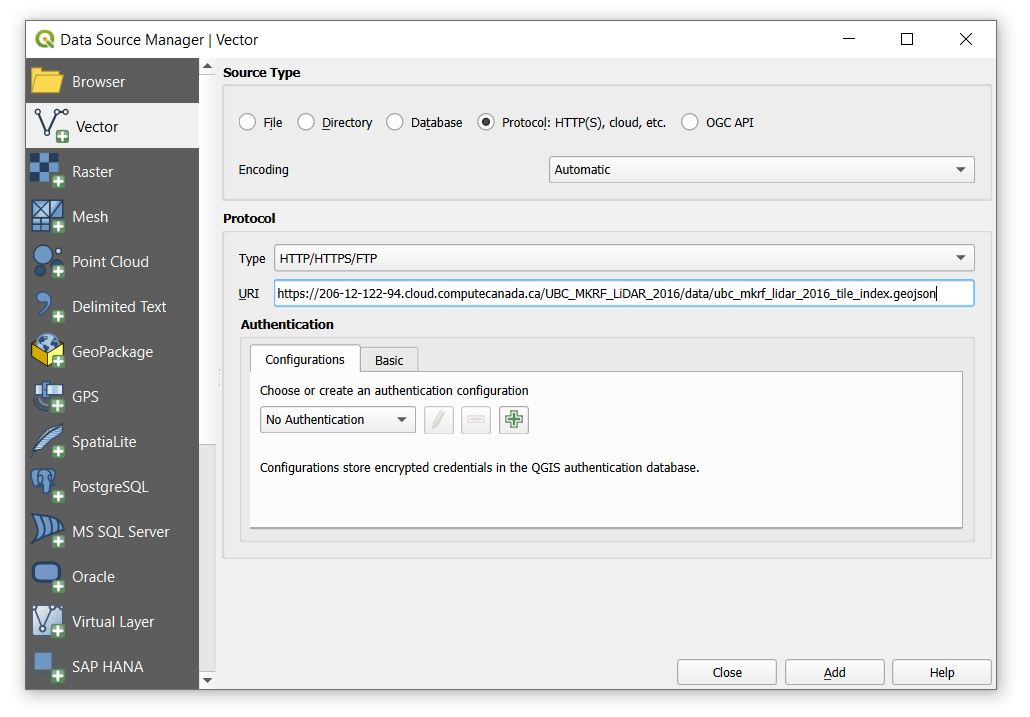
\includegraphics[width=0.75\linewidth]{images/01-qgis-data-source-manager-tile-index}

A nice feature about QGIS is that it supports the ability to read any openly-specified geospatial file directly from a remote source. ArcGIS Pro only allows you to read some sources published on compatible remote databases (e.g., ArcGIS enterprise geodatabase or PostgreSQL) or from layers published on ArcGIS Online.

Now that we have spatial tile metadata, we can perform spatial intersection to find the right tiles. Our AOI is going to be the following longitude-latitude bounding box:

Lower left (LL): -122.55275, 49.32325

Upper right (UR): -122.52506, 49.34135

\textbf{Step 4:} Open a notepad text editor and convert this bounding box into a geojson polygon feature with the following syntax:

\begin{verbatim}
{
  "type": "Polygon",
  "coordinates": [
    [
      [LL_longitude, LL_latitude],
      [UR_longitude, LL_latitude],
      [UR_longitude, UR_latitude],
      [LL_longitude, UR_latitude],
      [LL_longitude, LL_latitude]
    ]
  ]
}
\end{verbatim}

Replace with the correct longitude/latitude values. Note that this creates a square polygon and the fifth coordinate is the same as the first, which topologically encloses the polygon. Save the geojson in your QGIS project folder as ``mkrf\_aoi.geojson'' then open the file in QGIS. You should see that our AOI spans 16 total tiles.

\textbf{Step 4:} Click the ``Select by Location'' tool and ``Select features from'' the \textbf{ubc\_mkrf\_lidar\_2016\_tile\_index} layer by intersecting with the \textbf{mkrf\_aoi} you just made. Now the intersecting tiles are selected. Turn off \textbf{mkrf\_aoi} layer so that you can see the selection.

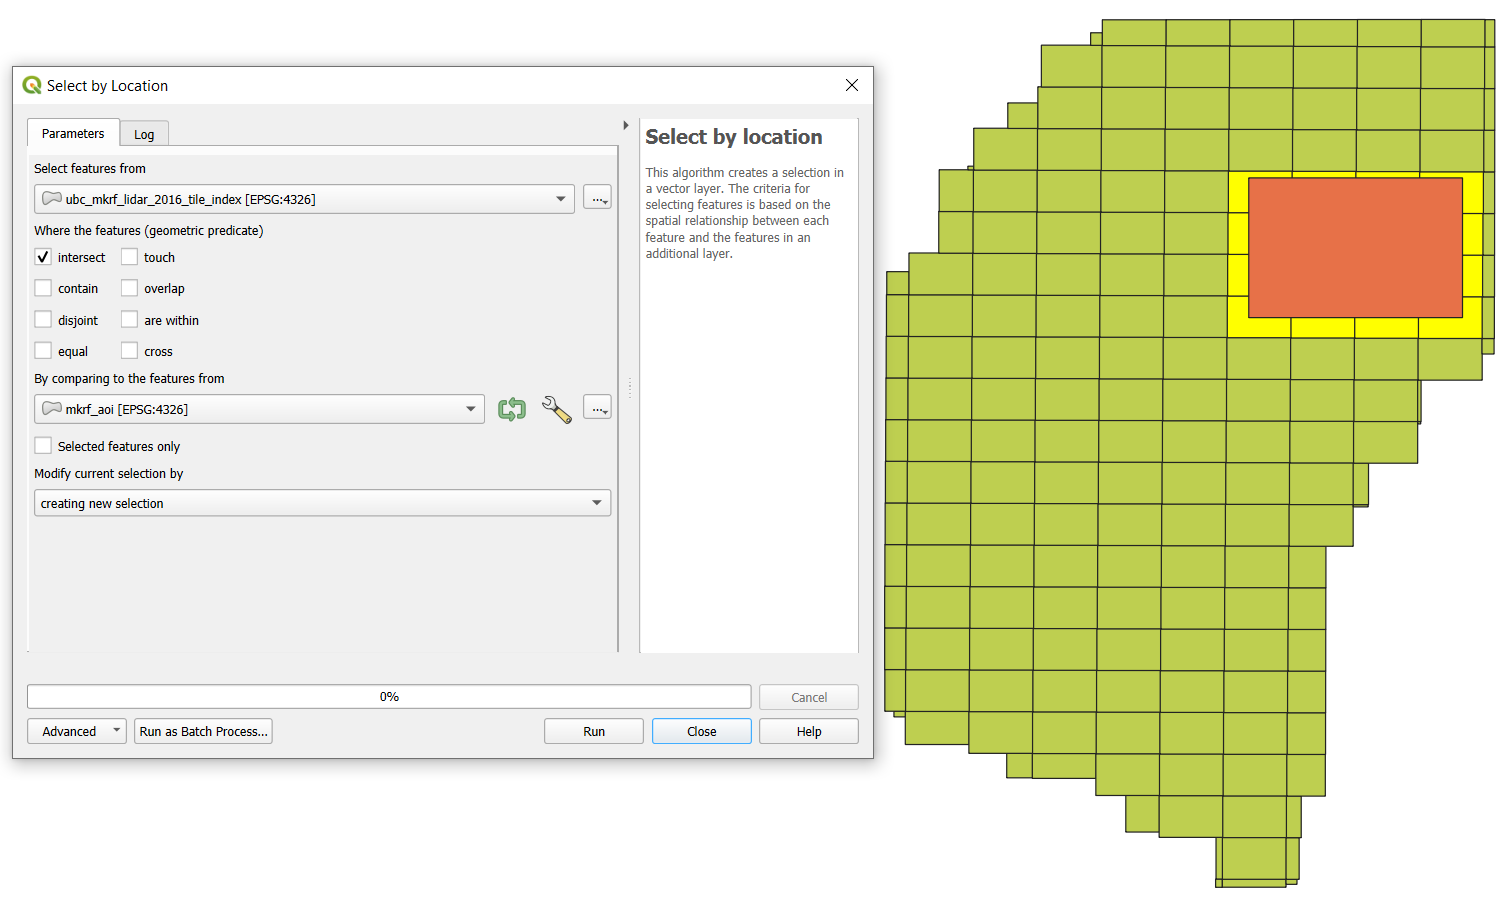
\includegraphics[width=0.75\linewidth]{images/01-qgis-intersect-aoi-tiles}

\textbf{Step 5:} Click the ``Identify Features'' tool and click on one of the selected tiles, which will highlight it in red and open the attributes for the polygon. Expand ``ubc\_mkrf\_lidar\_2016\_tile\_index'', ``url'', ``(Actions)'', and ``url''. Click the hyperlinked URL to download the tile to your QGIS project folder. Repeat this step for all 16 tiles.

\textbf{Step 6:} Add all of the downloaded tiles to your QGIS map canvas. The default symbology is the classification attribute, but only ground returns have been classified for the research forest.

However, the tiles are all still stored in separate files and some portions are outside our AOI. So next, we are going to filter, merge, and crop the point cloud, but we are going to do this outside of QGIS because it will be faster and more reliable. We are going to use the Point Data Abstraction Library (PDAL) command line utility to perform this processing. You can read more about the extensive PDAL functionality here: \url{https://pdal.io/} Note that many of the functions we are going to use with PDAL are available as tools through QGIS, but you have less control over the options and parameters in QGIS.

\textbf{Step 7:} Open the OSGeo4W shell and navigate to your QGIS project folder where your LiDAR data are located. For example, \texttt{cd\ C:\textbackslash{}users\textbackslash{}paul\textbackslash{}Documents\textbackslash{}QGIS\textbackslash{}mkrf\_lidar}. Type the command \texttt{pdal\ -\/-version} to make sure that PDAL was installed with your current version of QGIS. If a version number is returned in the console window, then continue to the next step, otherwise ask your instructor to help you install PDAL using the \href{https://trac.osgeo.org/osgeo4w}{OSGeo4W installer}.

PDAL can run functions in two ways. First, as subcommands, much like you have used with GDAL in prior labs. For example, \texttt{pdal\ merge\ {[}filename1.laz{]}\ {[}filename2.las{]}\ output.copc.laz} will use the \texttt{merge} subcommand and the file names that follow to merge many different las/laz/copc files together into the named output. Subcommands are generally good for small or incidental tasks like converting a file format or re-projecting data, but if you want to apply a more complex workflow then you should use a pipeline.

\href{https://pdal.io/en/2.6.0/pipeline.html\#pipeline}{Pipelines} are JSON-formatted files that give PDAL a set of instructions for reading, processing and writing point cloud data. With pipelines, you can define every step of the processing that you want and you can specify the finest level of detail at every stage. Pipelines are executed linearly, so we read the instructions from top-down. Below is an example of a pipeline that we are going to use, which is described in more detail below:

\begin{verbatim}
{
    "pipeline": 
        [
            "AQ11.copc.laz",
            "AQ12.copc.laz",
            "AQ13.copc.laz",
            "AQ14.copc.laz",
            "AR11.copc.laz",
            "AR12.copc.laz",
            "AR13.copc.laz",
            "AR14.copc.laz",
            "AS11.copc.laz",
            "AS12.copc.laz",
            "AS13.copc.laz",
            "AS14.copc.laz",    
            "AT11.copc.laz",
            "AT12.copc.laz",
            "AT13.copc.laz",
            "AT14.copc.laz",
            {
                "type":"filters.range",
                "limits":"Classification[2:2]"
            },
            {
                "type":"filters.crop",
                "bounds":"([-122.55275,-122.52506],[49.32325,49.34135])",
                "a_srs":"EPSG:4326"
            },
            {
                "type": "filters.merge"
            },
            {
                "type":"writers.las",
                "filename":"mkrf_aoi_lidar.las"
            }
        ]
}
\end{verbatim}

This pipeline will take all of our input tiles and filter, crop, merge, and write them out to a new file called ``mkrf\_aoi\_lidar.las''.

\begin{verbatim}
            {
                "type":"filters.range",
                "limits":"Classification[2:2]"
            },
\end{verbatim}

This first stage applies a \href{https://pdal.io/en/2.6.0/stages/filters.html}{filter} stage with a function called \href{https://pdal.io/en/2.6.0/stages/filters.range.html\#filters-range}{range}. Basically, this filter is telling PDAL that we only want the points that are classified as ground returns \texttt{Classification{[}2:2{]}} where \texttt{2:2} indicates the range of values from 2 to 2, which is the ground return classification code. So only ground returns are passed to the next stage:

\begin{verbatim}
            {
                "type":"filters.crop",
                "bounds":"([-122.55275,-122.52506],[49.32325,49.34135])",
                "a_srs":"EPSG:4326"
            },
\end{verbatim}

This next filter stage \href{https://pdal.io/en/2.6.0/stages/filters.crop.html\#filters-crop}{crops} the ground returns from the previous stage using the bounds of our AOI. We need to specify the spatial reference system \texttt{a\_srs} of these coordinates since the LiDAR data are in a projected coordinate system (EPSG:26910). So only ground returns that fall within our AOI are passed to the next stage:

\begin{verbatim}
            {
                "type": "filters.merge"
            },
\end{verbatim}

This next filter stage \href{https://pdal.io/en/2.6.0/stages/filters.merge.html\#filters-merge}{merges} all the ground returns in our AOI into a single stream, which is then passed to the last stage that writes it to an output file in LAS (uncompressed) format:

\begin{verbatim}
            {
                "type":"writers.las",
                "filename":"mkrf_aoi_lidar.las"
            }
\end{verbatim}

\textbf{Step 8:} Copy the contents of the pipeline to a text editor and save the file as ``process-lidar.json'' in your QGIS project folder.

\textbf{Step 9:} Return to the OSGeo4W shell and run the pipeline using the following command: \texttt{pdal\ pipeline\ process-lidar.json}. It may take several minutes for this step to complete, but in the end you should have a file called ``mkrf\_aoi\_lidar.las'' in your QGIS project folder. Drag it into QGIS and inspect it.

\begin{center}\rule{0.5\linewidth}{0.5pt}\end{center}

\hypertarget{task-2-visualize-lidar-data-in-qgis}{%
\section*{Task 2: Visualize LiDAR data in QGIS}\label{task-2-visualize-lidar-data-in-qgis}}
\addcontentsline{toc}{section}{Task 2: Visualize LiDAR data in QGIS}

The default symbology of LiDAR data in QGIS will be the classification, but we only have ground returns in our file, so everything will appear brown. Try symbolizing some of the other attributes like Intensity, ReturnNumber, and ScanAngleRank.

\textbf{Step 1:} Right-click the \textbf{mkrf\_aoi\_lidar} layer, open ``Properties'', select ``Symbology'' from the left, and then select ``Attribute by Ramp'' from the very top drop-down menu. Then choose your attribute and apply your symbology parameters. Make some notes of your observations for these attributes that you can reference in your report.

2D is a very boring way to visualize point cloud data, so let's create a 3D map view in QGIS.

\textbf{Step 2:} From the top menu, select ``View'', then ``3D map views'', and click ``New 3D Map View''. A small window will appear. Click and drag it to the top of your map canvas to dock it and make it larger.

\includegraphics[width=1\linewidth]{images/01-qgis-dock-3d-map-view}

\textbf{Step 3:} From the 3D map view menu bar, click the tool icon and toggle on ``Show Eye Dome Lighting''. Then, holding the \texttt{SHIFT} key, left-click and drag your cursor from top-to-bottom then release both buttons. This will give you an oblique shaded 3D perspective of the terrain.

\includegraphics[width=1\linewidth]{images/01-qgis-shift-up-down}

Navigating 3D data can be challenging using a 2D input device like a mouse, so we need to use different keyboard keys to control how we want to change our view:

\hypertarget{hold-shift-orbit-camera-around-fixed-position}{%
\subsection*{Hold SHIFT: Orbit camera around fixed position}\label{hold-shift-orbit-camera-around-fixed-position}}
\addcontentsline{toc}{subsection}{Hold SHIFT: Orbit camera around fixed position}

If you want to pan around a fixed position, then hold the \texttt{SHIFT} key and drag your cursor. The point cloud will rotate in the opposite direction. As you can see from the animation below, dragging your cursor in a circular pattern rotates the point cloud around a stationary imaginary point. If you continuously drag your cursor to the right, you will rotate around the fixed point counter-clockwise.

\includegraphics[width=0.75\linewidth]{images/01-qgis-shift}

\hypertarget{hold-ctrl-maintain-camera-position-and-change-camera-angle}{%
\subsection*{Hold CTRL: Maintain camera position and change camera angle}\label{hold-ctrl-maintain-camera-position-and-change-camera-angle}}
\addcontentsline{toc}{subsection}{Hold CTRL: Maintain camera position and change camera angle}

If you want to pan your camera angle up, down, left or right, then hold the \texttt{CTRL} key and drag your cursor in the direction you want to look. This only changes the camera angle, not the camera elevation or position.

\includegraphics[width=0.75\linewidth]{images/01-qgis-ctrl}

\hypertarget{hold-alt-move-camera-position-on-the-x-y-plane}{%
\subsection*{Hold ALT: Move camera position on the X-Y plane}\label{hold-alt-move-camera-position-on-the-x-y-plane}}
\addcontentsline{toc}{subsection}{Hold ALT: Move camera position on the X-Y plane}

If you find yourself wanting to move around, then hold the \texttt{ALT} key and drag your cursor in the direction that you want to move the camera. Think of this as sliding along an X-Y plane that is fixed at the camera elevation and angle.

\includegraphics[width=0.75\linewidth]{images/01-qgis-alt}

\hypertarget{scroll-move-camera-position-tofrom-the-cursor-location}{%
\subsection*{Scroll: Move camera position to/from the cursor location}\label{scroll-move-camera-position-tofrom-the-cursor-location}}
\addcontentsline{toc}{subsection}{Scroll: Move camera position to/from the cursor location}

If you want to move towards some feature, then simply point your cursor at it and scroll without clicking. This movement is akin to traversing a ray that connects your current camera position with a look direction angle (relative to X-Y-Z). Scrolling therefore changes the camera position and elevation. Scrolling down has the effect of ``zooming in'' while scrolling up has the effect of ``zooming out''. Be careful, though, because scrolling will always follow the current position of the cursor, so if you scroll down on one position and then move your cursor and scroll up, your camera position will not be where it started.

\includegraphics[width=0.75\linewidth]{images/01-qgis-scroll}

\textbf{Step 4:} Practice navigating in 3D and observing the different attributes across the ground surface. Make some notes of your observations for your report. There is a button on the top of the 3D map view to save an image of any given view.

\begin{center}\rule{0.5\linewidth}{0.5pt}\end{center}

\hypertarget{task-3-prepare-lidar-in-arcgis-pro}{%
\section*{Task 3: Prepare LiDAR in ArcGIS Pro}\label{task-3-prepare-lidar-in-arcgis-pro}}
\addcontentsline{toc}{section}{Task 3: Prepare LiDAR in ArcGIS Pro}

For this task, we will switch to ArcGIS Pro and practice manipulating the LiDAR point cloud to derive a terrain surface using different algorithms. ArcGIS Pro has several tools that we can use to view and analyse LiDAR point clouds. In order to view the dataset, we need to import it as a LAS Dataset. Note that QGIS with open LAS or LAZ files and immediately convert them to COPC format (.copc.laz), but ArcGIS Pro does not currently support reading COPC, so we must use the LAS file. If you want to reproduce this lab with other LiDAR data in ArcGIS Pro, you can convert LAZ to LAS using the ``Convert LAS'' tool.

\textbf{Step 1:} Open a new ArcGIS Pro map project and Search for the ``Create LAS Dataset'' tool. Specify the ``mkrf\_aoi\_lidar.las'' file as your input file. Make sure to name the output LAS Dataset and specify the correct coordinate system. Ensure that ``Create PRJ for LAS files'' is set to ``All LAS Files''. Toggle on ``Compute Statistics'' and run the tool. This will produce a LAS Dataset file (.lasd).

Pay attention to future steps of the lab as some tools expect the .lasd file while others expect the .las file!

\textbf{Step 2:} We can now add our LAS Dataset to the map. Depending on the zoom extent, you may only see the red bounding box of the LAS Dataset file; this is not an error, you just need to zoom in to see the actual points. Alternatively, you can open the dataset in a Local Scene, although due to the size of the point cloud this might cause some lag.

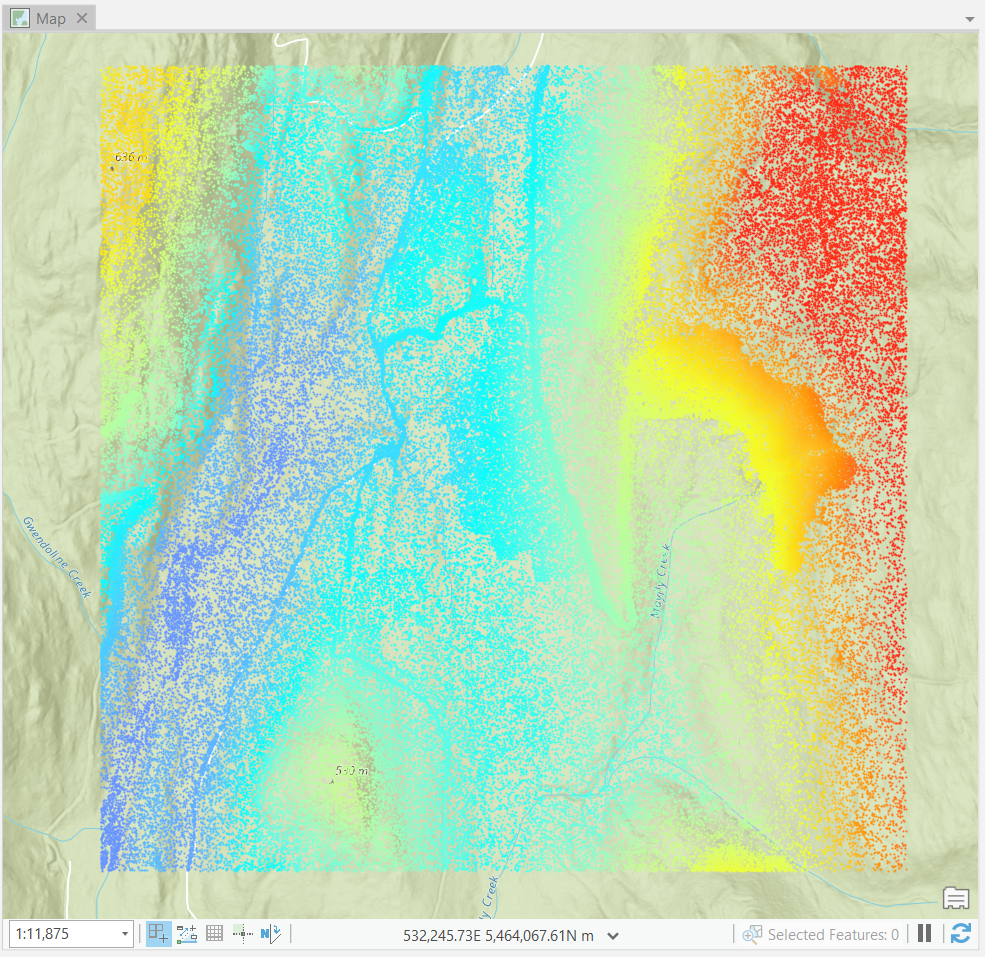
\includegraphics[width=0.75\linewidth]{images/01-arcgis-lasd}

\textbf{Step 3:} Another way to explore the dataset is to view the properties. Right-click the LAS Dataset and open the ``Properties''. Here we can see some statistics of the point cloud, such as information regarding the Classification Codes and Return Number. You can get more detailed metadata from a Catalog view. From the top ribbon, select the View tab and then click ``Catalog View''. Navigate to where you saved the LAS Dataset, right-click it, and open the ``Properties'' again.

Record these values:

\begin{itemize}
\item
  How many points are in the dataset?
\item
  What is the average point spacing?
\item
  What is the range of elevation?
\end{itemize}

\textbf{Step 4:} Search for the ``LAS Dataset to Raster'' tool, and use your LAS Dataset as the input. Since we are interested in creating a terrain surface model, we want to use the ``Binning'' ``Interpolation Type'', and make sure that we use the ``Minimum'' (i.e., the lowest ``Elevation'') points in each ``Cell Assignment'' of the output raster. ``Sampling Value'' refers to the resolution of the raster that we are creating, in other words, the spacing of our raster cell samples. Set the ``Sampling Value'' to 30 (meters), name the output raster ``MKRF\_DEM'' and run the tool.

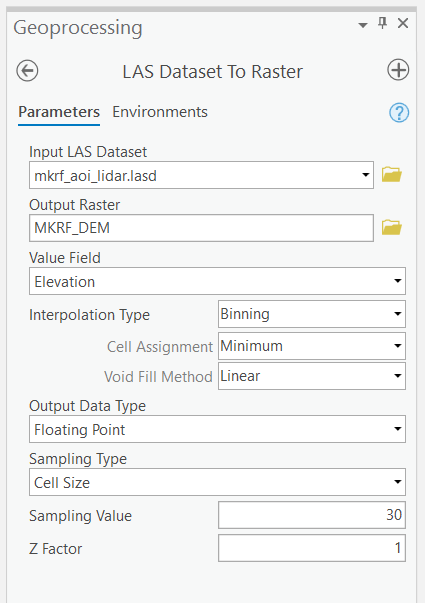
\includegraphics[width=0.5\linewidth]{images/01-arcgis-lasd-to-raster}

The tool above is the most straight-forward way to create a DEM from a LiDAR point cloud in ArcGIS Pro. It is also the least sophisticated and prone to error because it relies heavily on the presence of points. This is where spatial interpolation methods come in, but these analyses expect flat 2D points rather than a 3D point cloud; ``flat'' in the sense that the point is mapped on a horizontal datum only (X-Y) and the point elevation (Z) is stored as an attribute rather than a coordinate. This is a relatively minor technical detail, but an important one because you can spatially interpolate all other kinds of attributes that are not terrain.

\textbf{Step 5:} Search for the ``LAS to Multipoint'' tool. Input your LAS Dataset. You will notice that there is a box asking for the ``Average Point Spacing''. Enter the value that you recorded from the previous step. Set the correct coordinate system and then run the tool.

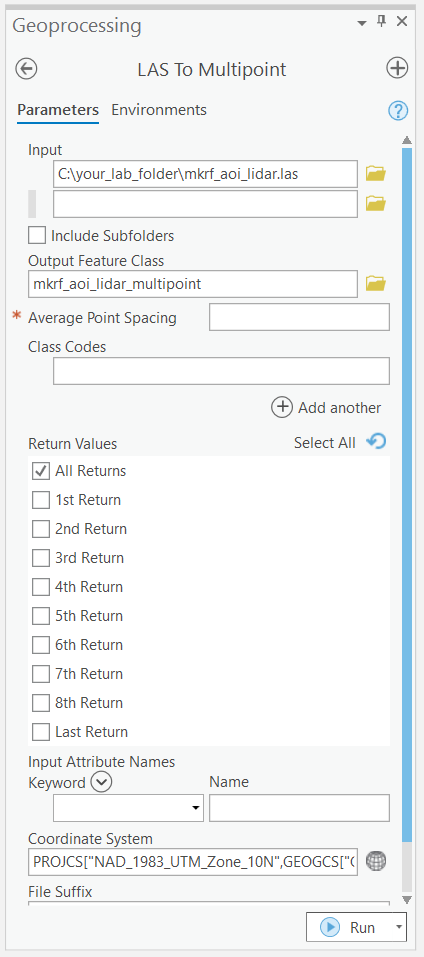
\includegraphics[width=0.5\linewidth]{images/01-arcgis-las-to-multipoint}

\textbf{Step 6:} Search for the ``Multipart to Singlepart'' tool. The multipoint feature class from the previous step is the input then run the tool.

\textbf{Step 7:} Now we need to add the Z value as an attribute. Search for the ``Add Z Information'' tool and use the singlepart features as the input. The only option available should be ``Spot Z'' and make sure it is toggled then run the tool.

We now have a 2D point feature class that we can use to test different spatial interpolation algorithms! ArcGIS Pro will attempt to draw the symbols for every single point in the multipart and singlepart feature classes, so keep them toggled off.

\begin{center}\rule{0.5\linewidth}{0.5pt}\end{center}

\hypertarget{task-4-apply-and-evaluate-spatial-interpolation-algorithms-in-arcgis-pro}{%
\section*{Task 4: Apply and evaluate spatial interpolation algorithms in ArcGIS Pro}\label{task-4-apply-and-evaluate-spatial-interpolation-algorithms-in-arcgis-pro}}
\addcontentsline{toc}{section}{Task 4: Apply and evaluate spatial interpolation algorithms in ArcGIS Pro}

Since we now have points representing height values, we can use the raster interpolation toolset to experiment with three different interpolation methods: Natural Neighbor, Inverse Distance Weighting (IDW), and Spline. You can read more about the tools we will be using from the \href{https://pro.arcgis.com/en/pro-app/tool-reference/spatial-analyst/an-overview-of-the-interpolation-tools.htm}{ArcGIS Pro documentation}.

Search for each of the interpolation tools listed above individually (for IDW, the tool is called ``IDW'') and explore their parameters. Natural Neighbor can be found with the ``LAS to Raster'' tool, change the ``Interpolation Type'' to ``Triangulation'', and ``Cell Assignment'' to ``Natural Neighbor''. Note that we will be using the 2D Spatial Analyst tools, not the 3D Analyst Tools.

\textbf{Step 1:} Create three rasters for each interpolation method: Natural Neighbor, IDW, and Spline. We suggest writing these rasters out to GeoTiffs so that you can also view them in QGIS, if you want. For each tool, keep the default settings, but make sure that you generate the rasters at 1 m resolution or whatever resolution you decided to run.

Take some time to inspect each raster, and look at their similarities and differences (make sure that you are using a common symbology when comparing). We can compare the differences between our interpolated rasters with the binned DEM that we created in the last task.

\textbf{Step 2:} In order to compare the rasters, we will make a raster of the differences between the interpolated surface and the binned DEM. You will use the ``Raster Calculator'' tool to do this. Subtract each interpolated surface from \textbf{MKRF\_DEM}. Name each difference raster according to the interpolation method: ``spline\_diff'', ``nn\_diff'', and ``idw\_diff''. We suggest writing these rasters out to GeoTiffs so that you can also view them in QGIS, if you want.

Next, we are going to quantitatively evaluate the differences and calculate statistics over different zones to see if there are any patterns or relationships with other variables.

\textbf{Step 3:} Use the ``Reclassify'' tool to reclassify the binned \textbf{MKRF\_DEM} into ``high'', ``medium'', and ``low'' areas. Use the range of elevation values that you recorded in the previous task from the LAS Dataset to decide the start and end ranges in the reclassification. Refer to the following table:

\begin{longtable}[]{@{}lll@{}}
\toprule\noalign{}
Start & End & New \\
\midrule\noalign{}
\endhead
\bottomrule\noalign{}
\endlastfoot
& & 1 \\
& & 2 \\
& & 3 \\
NODATA & NODATA & NODATA \\
\end{longtable}

\textbf{Step 4:} Use the ``Slope'' tool to create a raster called ``mkrf\_slope'' using degrees. Then, use the ``Reclassify'' tool to reclassify the degree slope values as follows:

\begin{longtable}[]{@{}lll@{}}
\toprule\noalign{}
Start & End & New \\
\midrule\noalign{}
\endhead
\bottomrule\noalign{}
\endlastfoot
0 & 15 & 1 \\
15.00001 & 30 & 2 \\
30.00001 & 90 & 3 \\
NODATA & NODATA & NODATA \\
\end{longtable}

We will use these reclassified areas as zones to calculate statistics about the difference between the interpolated surfaces and the binned DEM. For both zonations, higher values correspond to higher elevations and slopes.

\textbf{Step 5:} Search for the ``Zonal Statistics as Table'' tool. The ``Input Raster or Feature Zone Data'' are the reclassified zone rasters you just made. ``Zone Field'' should be ``Value''. The ``Input Value Raster'' is the raster that we want to summarize over the zones, which are all of the difference rasters we calculated in the earlier step. Run this tool for both each combination of the two topography zonations and the three difference rasters for the different interpolation methods. You should finish with six tables:

\begin{itemize}
\item
  idw\_diff\_elev
\item
  idw\_diff\_slope
\item
  nn\_diff\_elev
\item
  nn\_diff\_slope
\item
  spline\_diff\_elev
\item
  spline\_diff\_slope
\end{itemize}

\textbf{Step 6:} Create a hillshade from each of the interpolated surfaces using the ``Hillshade'' tool. Leave the default settings, which will illuminate the surface for a sun inclination (elevation) of 45° from a declination of 315° (northwest); unrealistic for this latitude at any time of year, but the cartographic standard nonetheless. Inspect the hillshades and use them to make additional observations for your report.

\textbf{Step 7:} Switch ArcGIS Pro to a Layout view. You may want to change the page orientation to landscape instead of portrait. To do so, go to ``File'' then ``Page and Print Setup''. In ArcGIS Pro, we can insert as many map frames as we want into our map layout. In our case, we will need 6 maps in our layout, as well as some free space for legends and text. There will be one interpolated surface and one difference raster for each of the three interpolation methods. Display each of these layers in their own map and place them appropriately in the layout. Each map should include only one raster, one of the following: DEMs using Spline, Natural Neighbor, and IDW, ``spline\_diff'', ``nn\_diff'', and ``idw\_diff''. Arrange the data frames by row and column so that the layout makes sense (that is, so each interpolation method is near one another.

\textbf{Step 8:} Add all of the tables from the previous step into one of the data frames. When you open these tables, you can add them to the map by clicking ``Table Options'' and selecting ``Add Table to Layout''. You can also remove unimportant columns from the display by right clicking the column name in the attribute table and clicking ``Turn Field Off''. Place the tables in the layout view a way that makes sense (near their respective difference raster). Label what each of the values means
with a text box (``Insert'' \textgreater{} ``Text'').

\textbf{Step 9:} Change symbology for both the overall and difference layers. Use the same symbology for all of them.

Start with the elevations. Click on one of the layers representing the interpolated surfaces (Spline, for example) and select the the Symbology tab. Change the Primary symbology to ``Classify''. Set the number of classes to 7. You may change the color ramp to one that makes sense to you, but make sure that there is enough contrast between classes. Change the symbology of the other two interpolated surfaces to match the first one (i.e.~make sure to match break classes). You can explore the ``Apply Symbology from Layer'' tool to do this quickly.

Repeat the same process for the difference rasters. This time, use 8 classes and set the breaks so that they make sense (e.g., 2, 4, 6, 8, 10, 12, 14, and 50).

Add a legend for each symbology definition (Elevation and Difference) to the map layout by clicking on a data frame and selecting ``Insert'' \textgreater{} ``Legend'' from the top menu bar. Place them on the map layout in a way that makes sense (near the respective layers).

Finally, put some text on the layout to communicate which data frame is which, and what each table represents. You can either label every data frame or label the columns and rows (``Interpolated Surface'' and ``Difference to DEM'' as rows and ``Spline'', ``Natural Neighbor'', and ``IDW'' as columns). Make sure you communicate what each aspect of the map is effectively! Save the map document and export the map document to a PNG (``Share'' \textgreater{} ``Export Layout'').

Note that the figure above uses slightly different data than this lab and should only be used as a reference to for the symbology and layout expectations, so your maps will look different.

\begin{center}\rule{0.5\linewidth}{0.5pt}\end{center}

\hypertarget{task-5-visualize-3d-data-in-arcgis-pro}{%
\section*{Task 5: Visualize 3D data in ArcGIS Pro}\label{task-5-visualize-3d-data-in-arcgis-pro}}
\addcontentsline{toc}{section}{Task 5: Visualize 3D data in ArcGIS Pro}

In this last brief task are some instructions for visualizing the point cloud and interpolated DEM surfaces in ArcGIS Pro. You can produce and export some 3D scenes that may help to illustrate your observations in your report.

\textbf{Step 1:} In ArcGIS Pro, click the ``Insert'' tab, click and expand ``New Map'', and select ``New Local Scene''.

\textbf{Step 2:} Add the ``mkrf\_aoi\_lidar.las'' file to the scene. Navigating an ArcGIS Pro scene is nearly the same as it is in QGIS. Though, instead of using keys on the keyboard to toggle between the different camera axes to manipulate, ArcGIS Pro provides an on-screen navigator in the bottom left. In this way, you can manipulate an ArcGIS Pro scene using just your mouse.

\includegraphics[width=1\linewidth]{images/01-arcgis-scene-navigation}

By default, ArcGIS Pro uses its own ``WorldElevation3D/Terrain3D'' source for the ``Ground'' in the Contents Pane. You can change the ground source to any DEM or really any other raster that you want to use the values of to create a ``ground'' surface. We are going to use this feature to explore the differences between the surface models we derived and the actual point cloud.

\textbf{Step 3:} Add the three interpolated DEM rasters to the scene and also the difference rasters. Toggle everything off in the scene. Drag the three DEM rasters under ``Ground''. Leave the three difference rasters under ``2D Layers''.

\textbf{Step 4:} For each difference raster, toggle it on and change the symbology to ``Stretch'', using a diverging ``Color Scheme'' and a ``Minimum Maximum'' ``Stretch Type''. Below in the ``Statistics'' tab, click ``Dataset'' and then select ``Custom'' from the drop-down menu. Modify the ``Minimum'' and ``Maximum'' values so that they are the same magnitude, but one is positive and the other is negative. You select the appropriate values based on the range of values that you observe in the difference raster and you will need to test different values to get your desired effect. For example, if the range of difference values is -10.51 and 21.32, then you might try setting the ``Minimum'' to -10 and the ``Maximum'' to 10. If you want the colors to be more apparent, then incrementally reduce the magnitude of your values: try -7, 7 next; then -5, 5; etc. until you reach your desired visualization. It it important to ensure that the midpoint is zero when using a diverging color scheme.

\textbf{Step 5:} Toggle on each pair of DEM (under ``Ground'') and difference raster (under ``2D Layers''). The ground source adds elevation to the difference raster that you symbolized, but does not impact or change the point cloud because it is inherently 3D data. Since we are using our own custom ground source, we can actually pan and observe a cross-section of the point cloud sitting on, above, or below the ground source and then observe local deviations between the point cloud and the derived DEM surface.

The white background might make it difficult to observe the differences. You can change the background color of the scene by left-clicking on ``Scene'' in the Contents Pane, open the ``Properties'', and then select the background color. We suggest using a light grey. There are other options for illumination that you can also modify in the ``Properties'', if you want. The image below shows an example of what the IDW might look like:

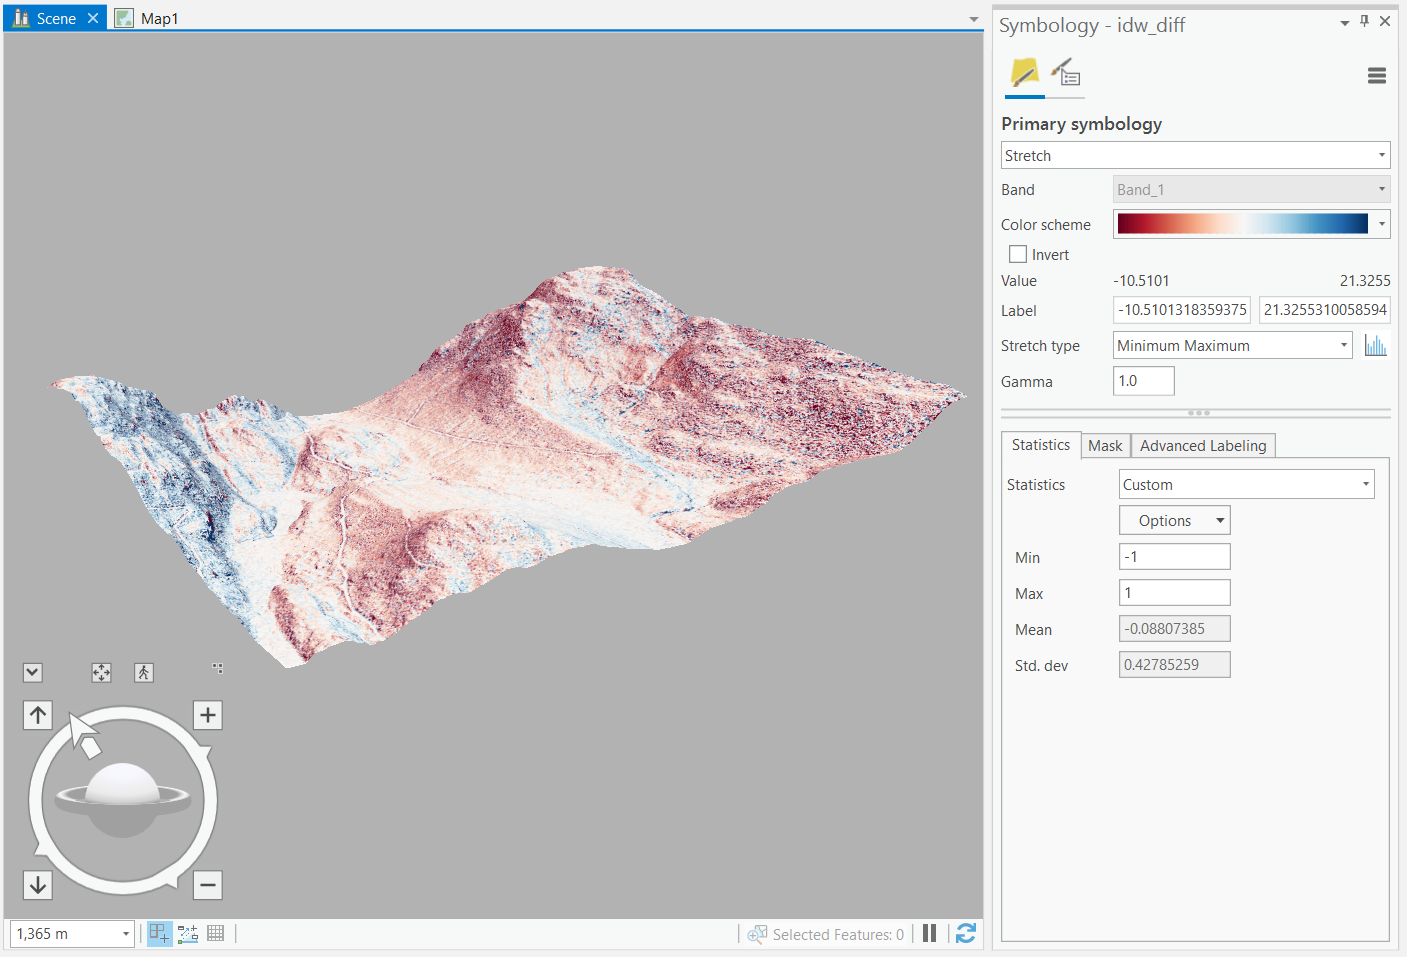
\includegraphics[width=1\linewidth]{images/01-arcgis-idw-diff}

Explore all of the DEM surfaces and export some examples that could help you interpret and illustrate your observations in your report.

\begin{center}\rule{0.5\linewidth}{0.5pt}\end{center}

\hypertarget{summary}{%
\section*{Summary}\label{summary}}
\addcontentsline{toc}{section}{Summary}

We covered a lot of ground in this lab about LiDAR processing with GIS software. One thing that should be apparent is that the vast majority of your time will be spent preparing LiDAR data for analysis. Point clouds are dense. Advances in scanning technology are creating new challenges for managing, accessing, organizing, and manipulating these dense data. Remember, we always want to work with the least amount of LiDAR data that our task requires. For spatial interpolation of terrain, this means only working with the necessary ground returns in our AOI. By filtering the tiles and points to only those we needed for the interpolation task, we reduced our data overhead by over 650\%!

You also practiced evaluating different spatial interpolation algorithms, which can have a large impact on subsequent analyses with those surfaces. When choosing an interpolation algorithm, you must always consider how dense your data are (i.e., how long will it take for me to produce this surface), what properties you want the output surface to have (i.e., statistical intervals, reproducing the true ranges, etc.), and what the surface will be used for (i.g., hydrology mapping, suitability analysis, etc.). Finally, you also practiced visualizing 3D data to augment and enhance your interpretations of these 2D interpolated surfaces.

Return to the \protect\hyperlink{lab1-deliverables}{\textbf{Deliverables}} section to check off everything you need to submit for credit in the course management system.

\hypertarget{network-analysis}{%
\chapter{Salmon Stream Network Analysis}\label{network-analysis}}

Written by
Paul Pickell

\hypertarget{lab-overview-1}{%
\section*{Lab Overview}\label{lab-overview-1}}
\addcontentsline{toc}{section}{Lab Overview}

An important application of GIS for watershed management is characterizing the physical components of streams, rivers, and water bodies. In this lab, you will learn how to use the Hydrology, Network Analyst, and Linear Referencing toolsets in ArcGIS Pro to extract hydrologic information from a digital elevation model (DEM) in order to model a network of streams.

In British Columbia, salmon are an important species for economic, cultural, and ecological reasons. Thus, there is extensive research and management efforts to better understand and sustainably manage salmon populations. There are five Pacific salmon species, Chinook, Coho, Chum, Pink, and Sockeye salmon. Salmon are diadromous species, spending their lifecycle in both freshwater and the ocean. We are particularly interested in habitat for salmon spawning. Salmon return to freshwater habitats to spawn and there are various requirements for salmon spawning that differ by species:

\begin{itemize}
\item
  Stream order
\item
  Proximity to a lake
\item
  Upwelling/downwelling
\item
  Water quality
\item
  Water depth
\item
  Water velocity
\item
  Substrate material
\item
  Slope gradient
\item
  Land cover
\end{itemize}

For this lab, you will identify the preferred habitat for salmon spawning based on proxy measures and how it corresponds to our stream network that we have derived from the DEM. This lab will walk you through how to measure stream order and slope. For your final report, you will also be expected to analyze an additional habitat requirement for salmon spawning. (Note: if you use some information that is not on the aforementioned list, please describe how it is a habitat requirement for salmon spawning in your report.)

In this lab, we will focus on Vancouver Island for a few reasons. First, islands make it possible to calculate flow accumulation exactly, which is important for creating a (nearly) topologically correct stream network. Second, Vancouver Island is large, which will enable us to look at natural sources of topological errors. Third, many species of Pacific salmon return to highly developed Vancouver Island to spawn and often come into conflict with human development.

\begin{center}\rule{0.5\linewidth}{0.5pt}\end{center}

\hypertarget{learning-objectives-1}{%
\section*{Learning Objectives}\label{learning-objectives-1}}
\addcontentsline{toc}{section}{Learning Objectives}

\begin{itemize}
\item
  Derive hydrology layers from a DEM
\item
  Model dams on streams as barriers by applying network topology
\item
  Evaluate a capability model of salmon habitat along stream segments using linear referencing
\item
  Trace a stream network and calculate reachable upstream salmon habitat
\end{itemize}

\begin{center}\rule{0.5\linewidth}{0.5pt}\end{center}

\hypertarget{lab2-deliverables}{%
\section*{Deliverables}\label{lab2-deliverables}}
\addcontentsline{toc}{section}{Deliverables}

Lab report with the following specification:

6 pages maximum PDF including figures, tables and references (3 points). Single-spaced, 12-point Times New Roman font (1 point). All figures and tables should be properly captioned (1 point).

Introduction should address the following questions and requirements (10 points):

\begin{itemize}
\item
  Describe network analysis and network topology.
\item
  What are some approaches to modelling reach within networks? Connectivity?
\item
  Reference to at least 3 peer review sources.
\end{itemize}

Methods should address the following requirements (10 points):

\begin{itemize}
\item
  Brief study area description and study area map showing the salmon conservation unit that you have selected to focus on.
\item
  Outline all primary steps included in the lab (no need to include exact ArcGIS Pro tool parameters).
\item
  Justify the use of specific methodological choices indicated in the lab.
\end{itemize}

Results should address the following questions and requirements (15 points):

\begin{itemize}
\item
  Map showing the reach of your streams from the ocean with dams as barriers
\item
  Zoom to Lake Cowichan. What is going on here? What could you do to automatically fix this for all large lakes?
\item
  How well do the streams you created line up with the mapped streams in the ArcGIS basemap?
\end{itemize}

Discussion should address the following questions and requirements (10 points):

\begin{itemize}
\item
  Comment on both small and large scale observations that you made throughout the process. Small scale observations would be investigating the behavior/structure of individual routes, while large scale observations would be the overall differences between total salmon habitat and habitat that can actually be reached from the ocean.
\item
  Discuss any limitations to the analysis based on your observations and suggest how the modelling process might be improved further. Illustrate your findings with figures, maps, and tables as needed. You are only expected to comment on a single conservation unit, but you may also run the entire island if you feel ambitious.
\item
  Consider how you might model the other salmon habitat requirements laid out at the beginning of the lab. Give brief examples for how you would model at least \ul{three of the criteria} that we \ul{did not} consider in the lab (i.e., do not discuss stream order, stream gradient). Assume that you have access to any typical data source (e.g., LiDAR, optical satellite, RADAR, land inventory, gauge stations, weather stations, etc).
\item
  How would you expect the stream network to change if you used a raster with a cell size of 5 m or 100 m?
\item
  How might additional topological errors and unidentified/unfilled sinks in the DEM impact your analysis?
\item
  What are your final recommendations to the province for conservation of spawning salmon habitat in Vancouver Island streams?
\item
  Reference to at least 3 peer review sources (can be the same sources as introduction).
\end{itemize}

\begin{center}\rule{0.5\linewidth}{0.5pt}\end{center}

\hypertarget{data-1}{%
\section*{Data}\label{data-1}}
\addcontentsline{toc}{section}{Data}

All data for this lab are accessible via the UBC PostgreSQL server. Instructions for connecting to the server are given in prior labs. We will be using data from the \texttt{salmon} database. To save time for this lab, the data have already been assembled and pre-processed for you, but below are some details about how that was achieved.

\textbf{vancouver\_island\_dem}

This was the general process applied to create the DEM in case you want to reproduce it or apply the same method for another project:

\begin{enumerate}
\def\labelenumi{\arabic{enumi}.}
\tightlist
\item
  Download all the tiles for Vancouver Island from the B.C. Government here
\item
  Mosaic the rasters together using the ``Mosaic to new raster'' tool
\item
  Buffer a polygon shapefile of Vancouver Island by 25 m
\item
  Convert the result of step 3 to a raster with cell size 25 m and project to NAD 1983 BC Environment Albers. This is a mask that extends just beyond the shore of Vancouver Island to account for mapping errors.
\item
  Extract the DEM from step 2 by the mask in step 4 to produce a DEM for only Vancouver Island that excludes all other nearby islands:
\end{enumerate}

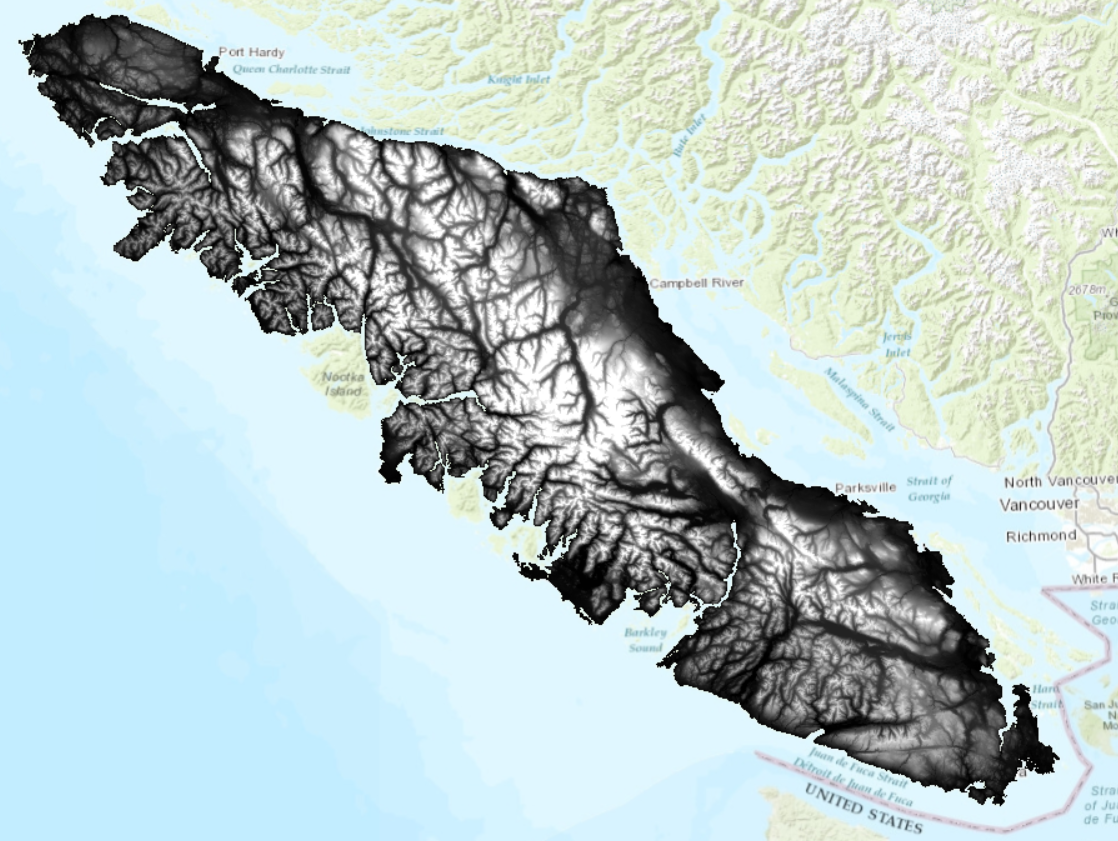
\includegraphics[width=0.75\linewidth]{images/02-vancouver-island-dem}

\textbf{vancouver\_island\_dem\_filled}

The DEM above was filtered several times for sinks. Generally, you can use the ``Fill'' tool to achieve this. However, Vancouver Island has many naturally-occurring geomorphic features that can cause real sinks (as opposed to random errors). In order to create a depressionless DEM, the DEM was iteratively put through the following process:

\begin{enumerate}
\def\labelenumi{\arabic{enumi}.}
\tightlist
\item
  Calculate flow direction
\item
  Calculate sinks
\item
  Calculate watersheds using the flow direction raster and the sinks raster as pour points
\item
  Calculate minimum elevation of the sinks using the ``Zonal statistics'' tool
\item
  Calculate maximum elevation of the watershed for the sink using the ``Zonal fill'' tool
\item
  Subtract result of step 4 from result of step 5 for the sinks mapped in step 2. This is the depth of each sink.
\item
  Add the sink depth to the DEM to fill the sink
\item
  Repeat steps 1-7 several times until you remove all sinks or achieve a stopping criterion
\end{enumerate}

The original DEM contained \textgreater3,000 sinks. After iterating the above 12 times, there were fewer than 300 sinks. You can subtract the DEM from the filled DEM to observe where fill was added. Notice any patterns for where sinks are located on the island?

\textbf{dams}

The dams were acquired from the BC Government \href{https://catalogue.data.gov.bc.ca/dataset/bc-dams}{here}. These data were clipped to Vancouver Island and represent dam structures as polyline features.

\textbf{Salmon conservation units (CU)}

Conservation units for Chinook, Chum, and Coho were acquired from Oceans and Fisheries Canada \href{https://open.canada.ca/data/en/dataset/1ac00a39-4770-443d-8a6b-9656c06df6a3\#wb-auto-6}{here}. These polygon areas were mapped considering ecology, life history, and molecular genetics (\href{https://onlinelibrary.wiley.com/doi/abs/10.1111/j.1095-8649.2001.tb01376.x}{Waples et al 2001}).

\begin{center}\rule{0.5\linewidth}{0.5pt}\end{center}

\hypertarget{task-1-create-stream-segments}{%
\section*{Task 1: Create stream segments}\label{task-1-create-stream-segments}}
\addcontentsline{toc}{section}{Task 1: Create stream segments}

Before starting the lab, you will need to download all of the data from the \texttt{salmon} database on the UBC PostgreSQL server and save it to your ArcGIS Pro project folder. You should save all of your outputs from the tools in this lab directly into your ArcGIS Pro project geodatabase. The reasoning for this is because we will only be working in ArcGIS Pro for this lab and also because the ArcGIS Pro topology tools only work with data inside an ArcGIS Pro geodatabase.

\textbf{Step 1:} Calculate the flow direction of the filled DEM, using the ``Flow Direction'' tool. The flow direction tool determines which raster cells flow into other cells based on the elevation difference the immediate neighborhood. Keep the defaults of the tool. Ensure that ``Force all edge cells to flow outward'' is toggled on and leave all other parameters with the default value.

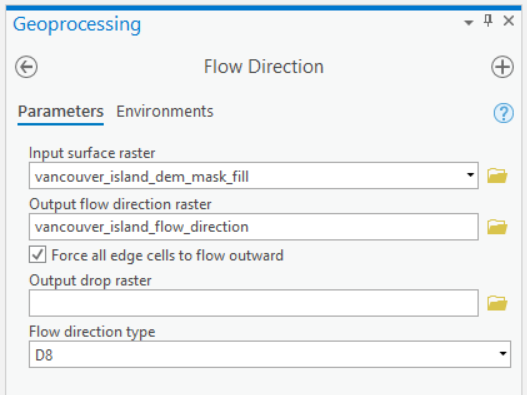
\includegraphics[width=0.5\linewidth]{images/02-flow-direction}

\textbf{Step 2:} Use the output from the ``Flow Direction'' tool as an input into the ``Flow Accumulation'' tool. Again, use the defaults within the tool, but select integer as the output data type because the output of this tool is a count. This tool will create a raster that represents the number of pixels that will accumulate into any given pixel. The bigger rivers will be displayed in the output. Play around with the symbology to visualize the stream network. (Hint: try using classify and various methods within symbology).

\textbf{Step 3:} To define streams, you need to set a threshold for the flow accumulation. Open ``Con'' and set the threshold or expression as any pixel that has a count of more than 1000. Therefore, any pixel that has a count of more than 1000 will be classified as a stream. For ``Input true raster or constant value'', use value 1. For ``Input false raster or constant value'', use value 0.

\textbf{Step 4:} Next, you will create a grid of stream links, which assigns unique values to each stream segment, so that the user can see how the streams are connected. Open the ``Stream Link'' tool and use the output from the ``Con'' tool and the flow direction raster here.

\textbf{Step 5:} You will also use the ``Stream Order'' tool using the same inputs as in step 4 and the default parameters. The ``Stream Order'' tool assigns a numeric order to segments of the raster, essentially classifying branches of the stream network.

\textbf{Step 6:} You will also convert your raster into polylines using the stream links raster and flow direction raster as inputs for the ``Stream to Feature'' tool. Toggle off ``Simplify polylines''.

Below is a useful flowchart of the process of creating a stream network from a DEM (\href{https://pro.arcgis.com/en/pro-app/tool-reference/spatial-analyst/deriving-runoff-characteristics.htm}{Source})

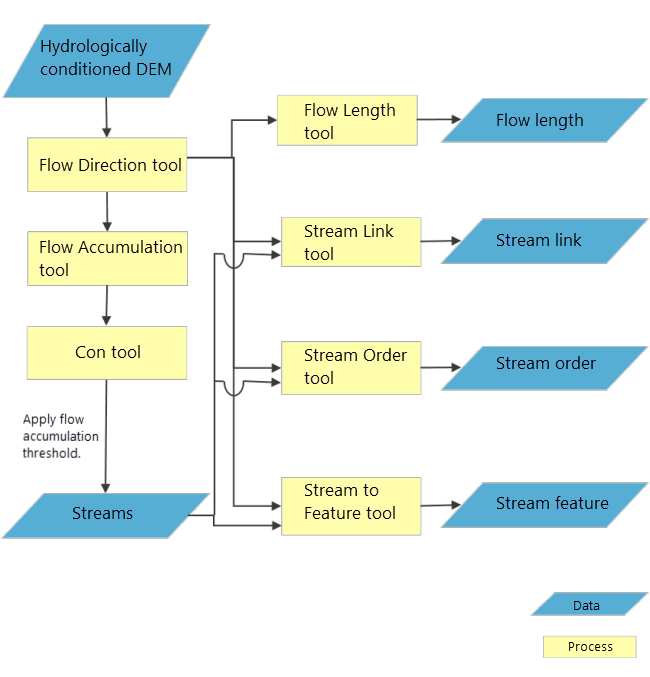
\includegraphics[width=0.75\linewidth]{images/02-flow-chart}

\begin{center}\rule{0.5\linewidth}{0.5pt}\end{center}

\hypertarget{task-2-create-routes-and-apply-topology}{%
\section*{Task 2: Create routes and apply topology}\label{task-2-create-routes-and-apply-topology}}
\addcontentsline{toc}{section}{Task 2: Create routes and apply topology}

At this point, you have only created polyline features representing streams. Next will convert those segments to routes and apply topology for our streams, as well as incorporate dams into the network.

\textbf{Step 1:} Convert your stream features into routes using the ``Create routes'' tool. Set the Route ID field to ``arcid''. The coordinate Priority parameter can be set to any corner.

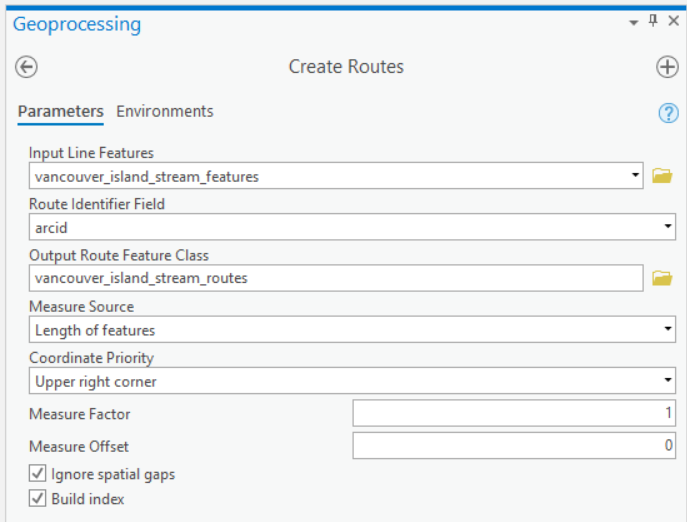
\includegraphics[width=0.5\linewidth]{images/02-create-routes}

\textbf{Step 2:} Create a new feature dataset in your geodatabase. Right-click your geodatabase in the Catalog pane and select New Feature Dataset. For the projection, use NAD 1983 BC Environment Albers.

\textbf{Step 3:} Import the stream routes and dams feature classes to the feature dataset within the Catalog view.

The dams are modelled as polylines. We need to identify where these dams intersect the stream routes. We want to return a single point for that location so that we can properly model the dams in our network. We will use topology to achieve this.

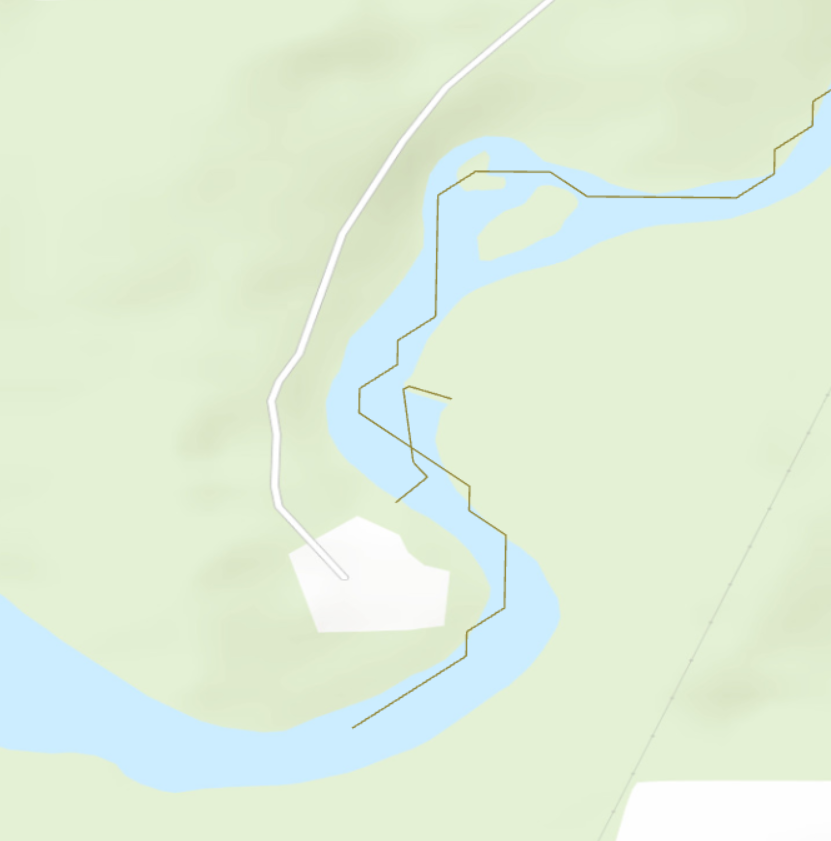
\includegraphics[width=0.5\linewidth]{images/02-example-dam}

\textbf{Step 4:} Right-click the feature dataset and select ``New'' and ``Topology''. This will open the Create Topology Wizard dialogue box.

\textbf{Step 5:} On the first page of the wizard, toggle on the dams and stream routes feature classes.

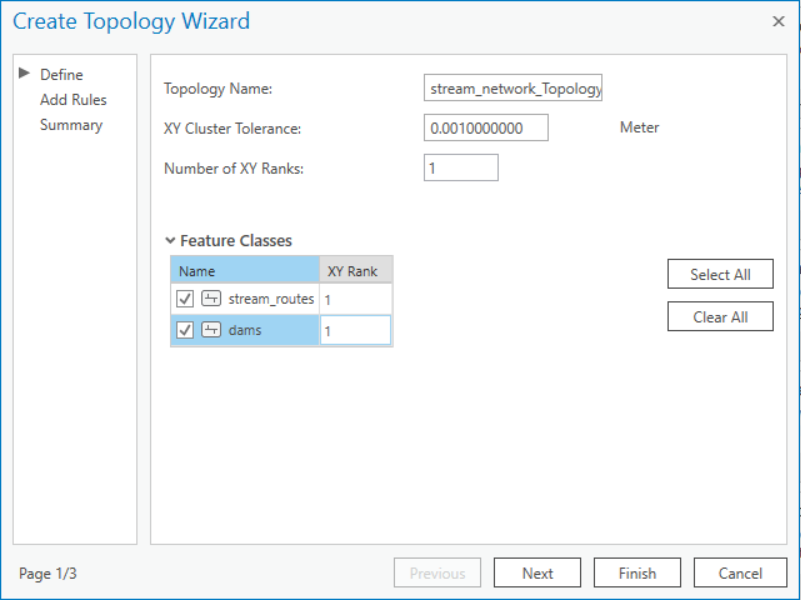
\includegraphics[width=0.75\linewidth]{images/02-create-topology-1}

\textbf{Step 6:} On the second page of the wizard, add a new rule so that the stream polylines must not intersect with the dam polylines.

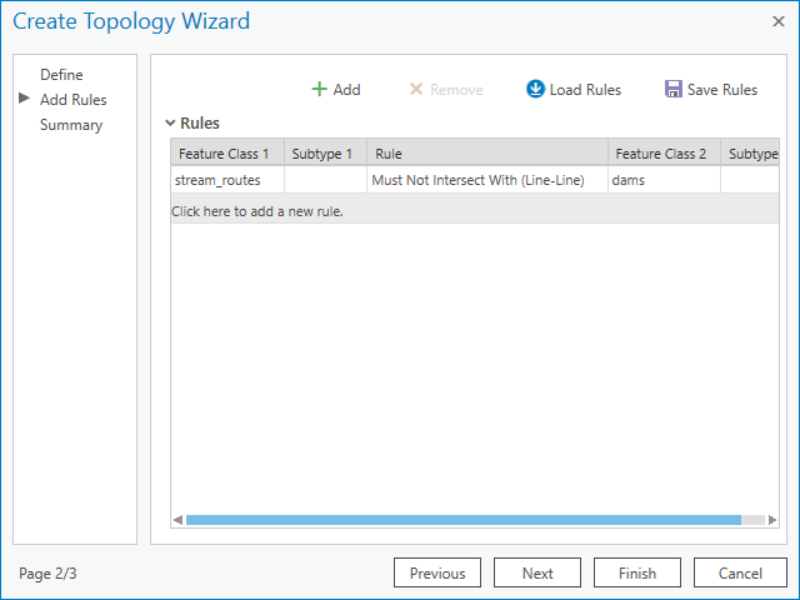
\includegraphics[width=0.75\linewidth]{images/02-create-topology-2}

Once done, click ``Finish''.

\textbf{Step 7:} Validate the topology by right-clicking the topology in the feature dataset and clicking ``Validate''.

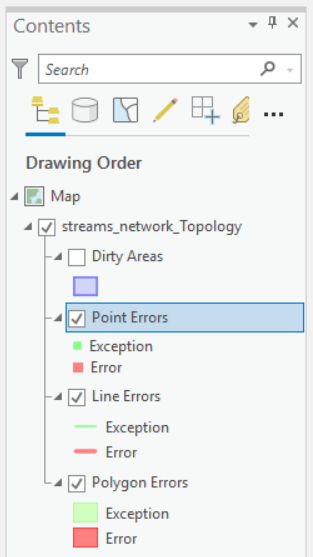
\includegraphics[width=0.5\linewidth]{images/02-topology-errors}

\textbf{Step 8:} You can click and drag the topology into the map to view any errors. We expect there to be errors because we know that the dams should intersect with our stream routes. You should see red squares all over the island. In the Contents Pane, right-click the ``Point Errors'' layer, select ``Data'', and select ``Export Features''. Save the points to your feature dataset as ``stream\_dam\_junctions''.

At this point, take a moment to appreciate where we are in this problem. We have modelled streams as routes and we now know where dams intersect with those routes. Salmon are diadromous species, they swim from the saltwater ocean up the freshwater streams to spawn. Therefore, we need one more piece of information in order to model how salmon swim upstream. We need to know where the streams meet the ocean.

\textbf{Step 9:} Take the Vancouver Island boundary polygon provided and perform a negative buffer, called a nibble. Use -25 meters for the buffer distance. We are doing a negative buffer because we want to ensure that this edge intersects with the streams that terminate at the ocean. Remember that the streams were generated by an imperfect and imprecise DEM, therefore this process will ensure that every stream that reaches the ocean will intersect this boundary.

\textbf{Step 10:} Convert the nibbled Vancouver Island boundary to a polyline using the ``Polygon to line'' tool. Be sure to toggle off ``Identify and store polygon neighboring information''. Save the result to your feature dataset.

Next, we will use the same topology process to identify where the island boundary intersects the stream routes.

\textbf{Step 11:} Right-click the network topology and select ``Properties''. This will open the topology wizard dialogue again. On the left, select ``Feature Class'' and toggle on the nibbled Vancouver island boundary that you created in step 10 and the stream routes. Toggle everything else off. On the left, select ``Rules''. Highlight the previous rule and click the ``Remove'' button at the top. Then, add a rule so that the stream routes must not intersect with the nibbled island boundary. Refer to steps 5 and 6 above if you need clarification.

\textbf{Step 12:} Again, validate the topology, add the topology to the map view, and export the Point Errors to a point feature class in your feature dataset. Name it ``stream\_ocean\_junctions''. Refer to steps 7 and 8 if you need clarification.

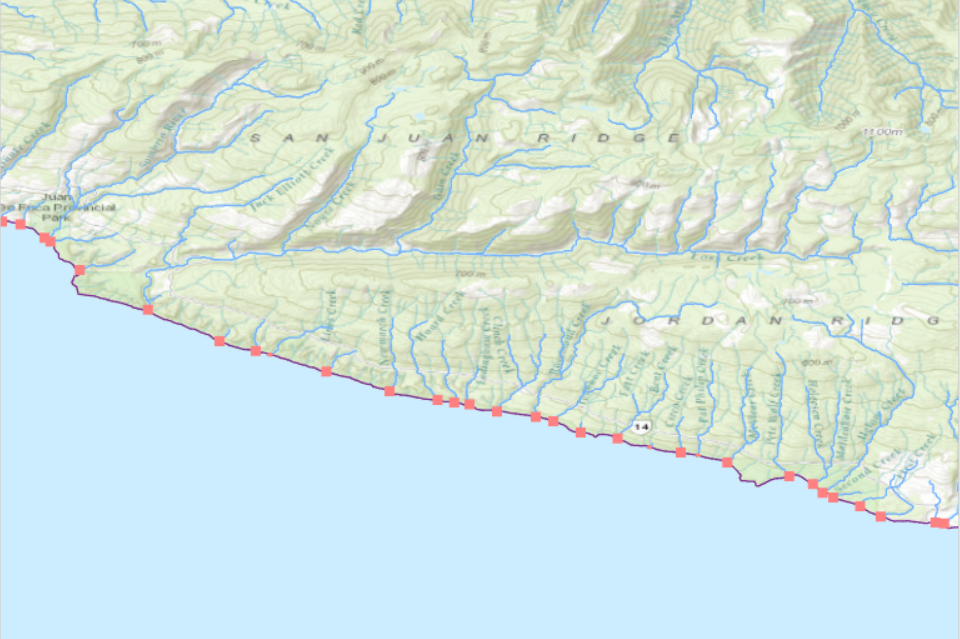
\includegraphics[width=1\linewidth]{images/02-ocean-stream-junctions}

\begin{center}\rule{0.5\linewidth}{0.5pt}\end{center}

\hypertarget{task-3-record-stream-attributes-with-linear-referencing}{%
\section*{Task 3: Record stream attributes with linear referencing}\label{task-3-record-stream-attributes-with-linear-referencing}}
\addcontentsline{toc}{section}{Task 3: Record stream attributes with linear referencing}

Now that we have stream routes, we can calculate some information that relate to salmon habitat. Water quality is important for salmon spawning habitat. Steeper gradients (slope) may be more susceptible to erosion that could be one proxy for lower water quality. In this task, you will practice extracting information about the streams and storing that information in the routes using linear referencing.

\textbf{Important:} Some of these operations can be computationally intensive because we will be dealing with up to 10\textsuperscript{5} features for the entire island. The instructions that follow are demonstrated on the entire island network dataset. You can attempt to process the entire island, but ultimately \ul{you need to clip your stream routes to one of the conservation units} (CU) for any of the three species of salmon for your report.

\textbf{Step 1:} Calculate the slope of the filled DEM using ``Percent rise'' as the output measurement and ``Planar'' as the Method.

\textbf{Step 2:} Now use the ``Extract by Mask'' tool to extract the slope raster by the mask of the stream links raster you created back in Task 1. This will produce a raster with slope values only where our streams exist.

\textbf{Step 3:} In British Columbia, stream gradients \textless{} 20\% are generally considered to be fish-bearing. Therefore, use the ``Reclassify'' tool to classify slopes \textless{} 20\% to a value of 1 and all other slopes to a value of 0.

\textbf{Step 4:} Use the ``Stream to Feature'' tool to convert the classified slope raster to line features. Parameterize this tool similar to the way you did in Task 1:

\begin{itemize}
\item
  Input stream raster is the classified slope raster you just made in step 3
\item
  Input flow direction raster is the original flow direction raster you made in Task 1
\item
  Name the output ``stream\_features\_slope\_classified''
\item
  Uncheck ``Simplify polygons''
\end{itemize}

Now you have another feature class of streams that should spatially match your stream routes, but these new polylines contain the gradient information. Now we will overlay this information with the routes.

\textbf{Step 5:} Use the ``Locate Features Along Routes'' tool to overlay the gradient information with the routes.

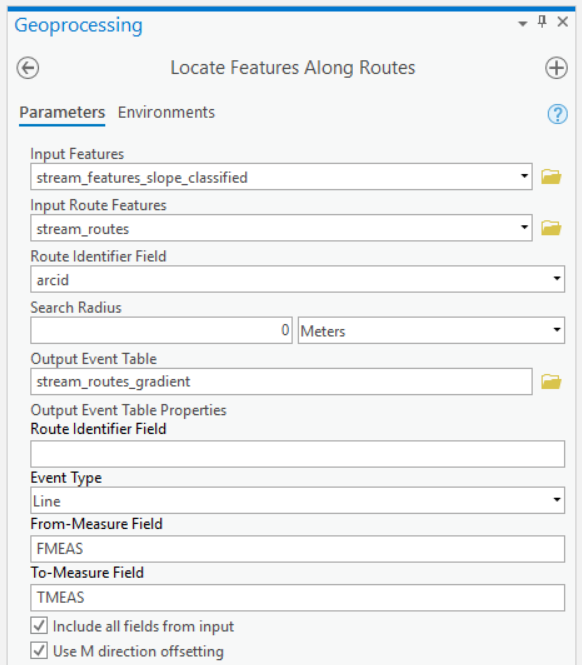
\includegraphics[width=0.5\linewidth]{images/02-locate-features-along-routes}

This will produce a route event table that should look something like this:

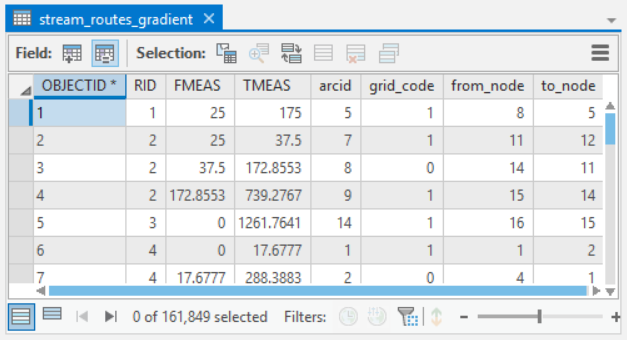
\includegraphics[width=0.5\linewidth]{images/02-stream-routes-gradient}

grid\_code in the event table represents the classified stream gradient (0 is ≥20\%, 1 is \textless20\%). Note that you have more records in this table than you have routes, because many routes are being segmented based on the gradient. Thus, you see repeating route id''s (RID).

Add a Short field to the event table called ``GRADIENT'' and calculate this field as !grid\_code! to transfer the grid\_code values to a more meaningful field name.

\textbf{Step 6:} Repeat steps 4 and 5 above for the stream order raster that you generated in Task 1. Ensure that the stream\_order raster is used as the ``Input stream raster'' and ``Simplify polygons'' is toggled off. In the end, you should have a second event table where the grid\_code (values between 1 and 6) indicates the stream order for each route. Again, add a Short field to the event table called ``SORDER'' and calculate this field as !grid\_code! to transfer the grid\_code values to a more meaningful field name.

\begin{center}\rule{0.5\linewidth}{0.5pt}\end{center}

\hypertarget{task-4-trace-the-network}{%
\section*{Task 4: Trace the network}\label{task-4-trace-the-network}}
\addcontentsline{toc}{section}{Task 4: Trace the network}

Now we can create a network that will allow us to trace the routes from the ocean to the dams.

\textbf{Step 1:} Open the ``Create Trace Network'' tool:

\begin{itemize}
\item
  The Input Feature Dataset should point to your feature dataset in your geodatabase
\item
  Trace Network Name can be named ``stream\_trace\_network''
\item
  Input Junctions should contain both the ``stream\_dams\_junction'' and ``stream\_ocean\_junctions'' that you created in steps 8 and 12 from Task 2
\item
  Input Edges should contain the stream routes and set the Connectivity Policy to ``Complex edge''
\end{itemize}

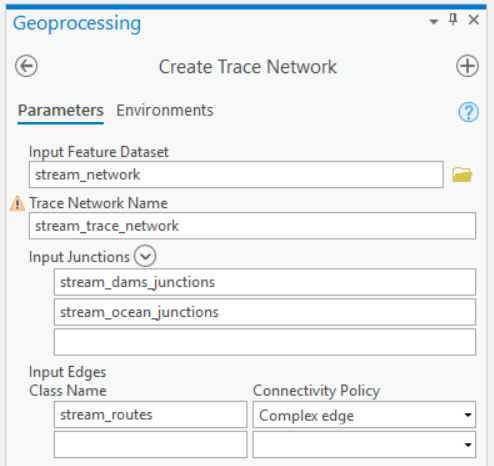
\includegraphics[width=0.5\linewidth]{images/02-create-trace-network}

\textbf{Step 2:} Run the ``Enable Network Topology'' tool on the trace network you just created.

\textbf{Step 3:} Run the ``Validate Network Topology'' tool on the trace network you just created. You might receive a warning: "A dirty area is not present within the specific extent." Ignore it.

\textbf{Step 4:} Open the ``Trace'' tool. This tool traces a path along a network the meets specified criteria. It also supports modelling barriers, so that the tracing terminates when a barrier feature is reached. Here is how we will parameterize this tool:

\begin{itemize}
\item
  Input Trace Network is the trace network that you created earlier
\item
  Trace Type is ``Connected''
\item
  Starting Points are the ``stream\_ocean\_junctions'' that you created earlier
\item
  Barriers are the ``stream\_dam\_junctions'' that you created earlier
\item
  Toggle on ``Include Barrier Features''
\item
  Toggle off ``Validate Consistency''
\item
  Toggle off ``Ignore Barriers at Starting Points''
\item
  Leave all Advanced Options as defaults
\end{itemize}

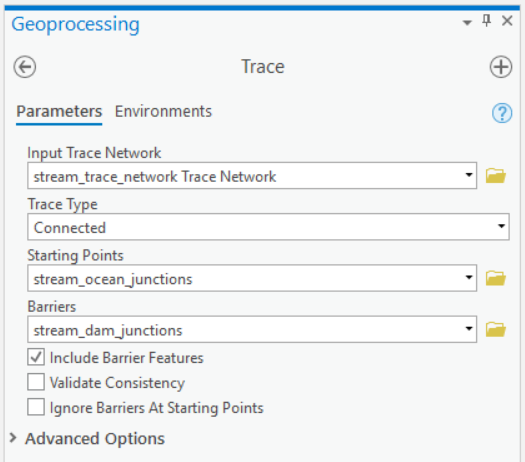
\includegraphics[width=0.5\linewidth]{images/02-trace}

\textbf{Step 5:} Once you have ran the ``Trace'' tool, you will see some of the routes selected on your map. Add a Short field to the route attribute table called ``REACHED''. Calculate this field with a value of ``1'' for the routes selected. Invert the selection and calculate the field again for the selected features with a value of ``0''. Finally, clear the selection and symbolize the routes based on the ``REACHED'' field. Congratulations! You have now modelled which route segments can be reached from the ocean before running into a dam. Your stream\_routes should look something like this (blue = unimpeded streams, yellow = stream reaches that are impeded by a dam):

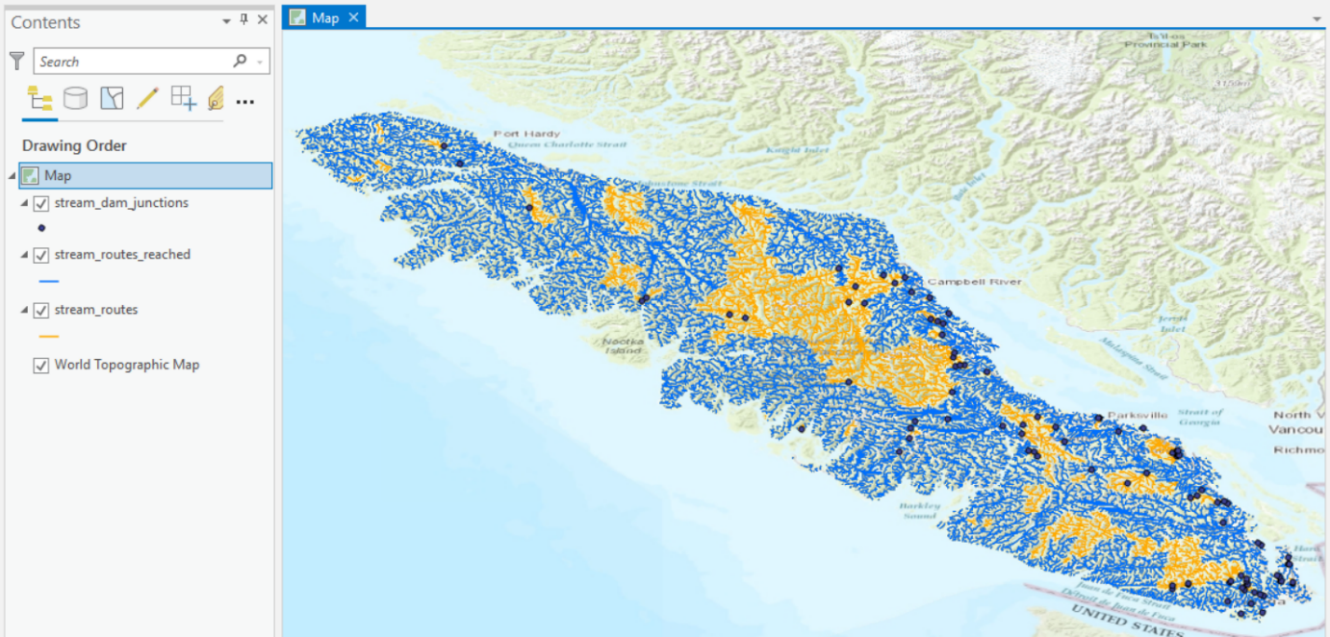
\includegraphics[width=0.75\linewidth]{images/02-traced-network}

\textbf{Important:} If your map looks significantly different from above, like most of the streams are impeded, then try these fixes:

\begin{itemize}
\item
  Zoom in closely to the ocean and dam junctions to ensure they are overlapping with the stream routes.
\item
  Apply a new topology rule that dam/ocean junctions must be coincident with the stream routes.
\item
  If there are any errors from above, then use the ``Snap'' tool to force the ocean and dam junctions to. The input features are the features that you want to move (snap), in this case the ocean and dam junction points. The type should be set to ``Edge'' and usually a distance of 25-30 meters is sufficient, but check the output
\item
  If you are still having trouble, try deleting the Trace Network from the feature dataset and rebuilding it (``Create Trace Network'' + ``Enable Network Topology'' + ``Validate Network Topology'').
\item
  If you are unable to delete the trace network, your geodatabase may be corrupt. Try creating a new geodatabase and import or re-create the important feature classes. Then, re-create the feature dataset and rebuild the trace network.
\end{itemize}

\begin{center}\rule{0.5\linewidth}{0.5pt}\end{center}

\hypertarget{task-5-overlay-and-query-the-network}{%
\section{Task 5: Overlay and query the network}\label{task-5-overlay-and-query-the-network}}

Now you will practice doing an overlay with your route event tables to transfer all the attributes into a common linear referencing system. This will allow you to then query the network for stream segments that meet some basic conditions for salmon habitat.

\textbf{Step 1:} Parameterize the ``Overlay Route Events'' tool like below:

\begin{itemize}
\item
  Input Event Table is your classified gradient event table from Task 3
\item
  Overlay Event Table is the stream order event table from Task 3
\item
  From-Measure Field is FMEAS
\item
  To-Measure Field is TMEAS for both input event tables and the output event table
\item
  Type of Overlay is Intersect
\item
  Name the Output Event Table ``stream\_route\_overlay''
\item
  Leave the Route Identifier Field empty for the output, but ensure it is set to RID for both the input tables
\end{itemize}

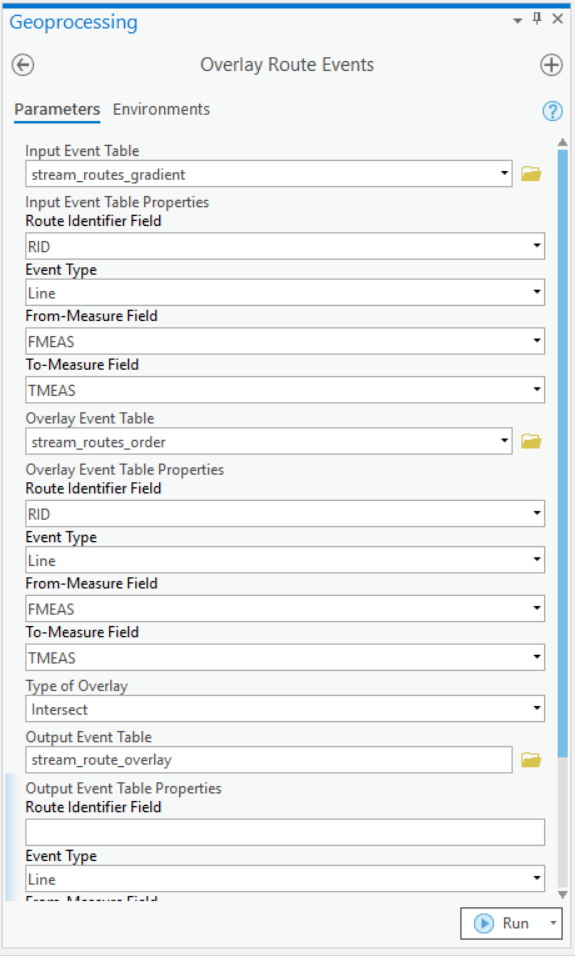
\includegraphics[width=0.5\linewidth]{images/02-overlay-route-events}

This will produce a new output event table that contains the intersection of stream gradient and stream order along the routes. As well, this event table should contain which routes can be reached from the ocean before running into a dam. Keep in mind that this is just a table, not a feature class. This is known as \emph{dynamic segmentation}. Next we will add one last field, visualize the everything and do a simple query.

\textbf{Step 2:} Join the field ``REACHED'' from the original routes to the overlay event table you just created using the ``Join Field'' tool:

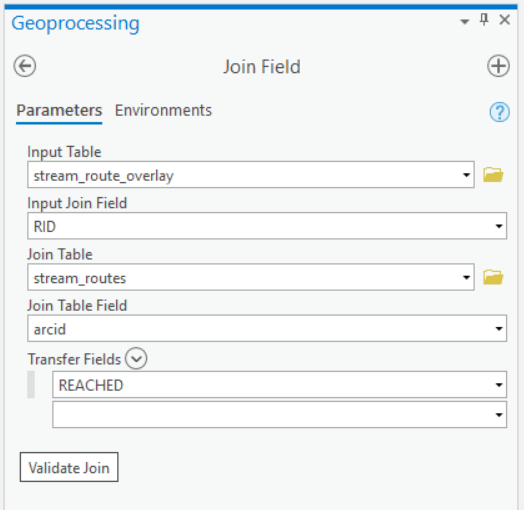
\includegraphics[width=0.5\linewidth]{images/02-join-field}

You should now have a table that has all the fields we need: SORDER, GRADIENT, and REACHED. (Note that some fields have been hidden from view in the table below.)

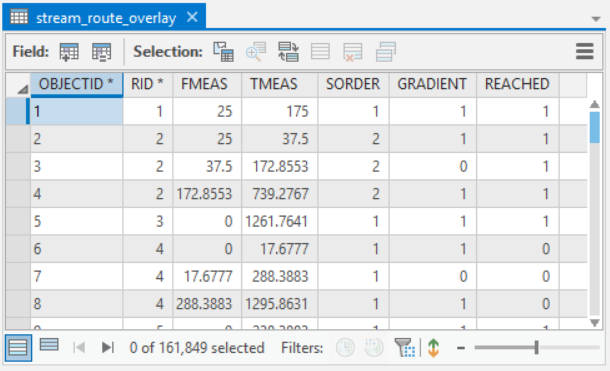
\includegraphics[width=0.75\linewidth]{images/02-stream-route-overlay}

\textbf{Step 3:} Use the ``Make Route Event Layer'' tool to convert the output event table to a feature class. Parameterize the tool as follows:

\begin{itemize}
\item
  Input route features will be the routes you originally created in Task 1
\item
  Route identifier field is ``arcid''
\item
  Input event table is the ``stream\_route\_overlay'' table that you created from step 1
\item
  From-measure field is ``FMEAS''
\item
  To-measure field is ``TMEAS''
\item
  Layer name or Table view is ``stream\_route\_overlay\_layer''
\end{itemize}

\textbf{Step 4:} Query the event layer from step 2 for stream segments with the following requirements:

\begin{itemize}
\item
  \ul{\textbf{Can}} be reached from the ocean
\item
  Is 1\textsuperscript{st} or 2\textsuperscript{nd} order stream
\item
  Has a gradient not steeper than 20\%
\end{itemize}

Export the selected features to a new feature class called ``accessible\_salmon\_habitat''.

\textbf{Step 5:} Repeat the query using the following requirements:

\begin{itemize}
\item
  \ul{\textbf{Cannot}} be reached from the ocean
\item
  Is 1\textsuperscript{st} or 2\textsuperscript{nd} order stream
\item
  Has a gradient not steeper than 20\%
\end{itemize}

Export the selected features to a new feature class called ``inaccessible\_salmon\_habitat''.

If everything goes \emph{swimmingly}, then the selected stream segments that meet the habitat criteria and can be reached from the ocean will look something like this:

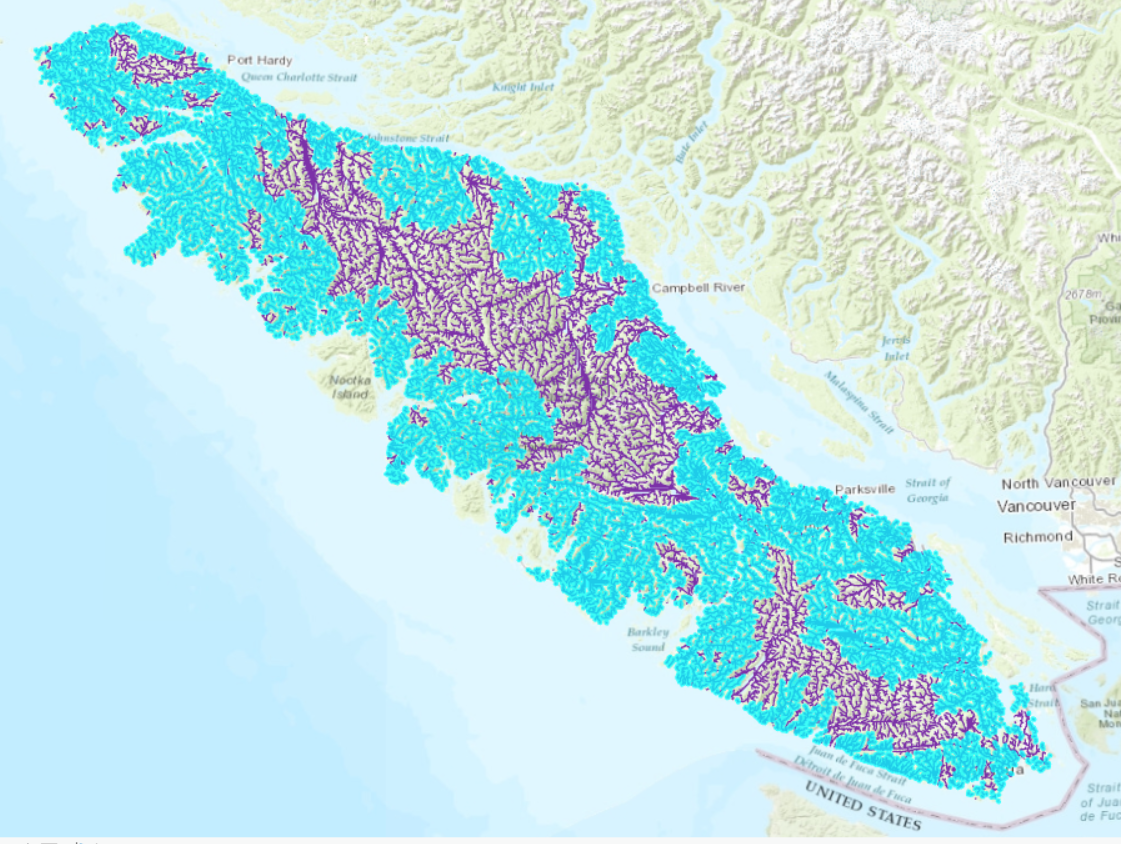
\includegraphics[width=1\linewidth]{images/02-selected-streams}

\begin{center}\rule{0.5\linewidth}{0.5pt}\end{center}

\hypertarget{summary-1}{%
\section*{Summary}\label{summary-1}}
\addcontentsline{toc}{section}{Summary}

Would you have guessed that you could do all that analysis from a single DEM? That is the power of applying focal functions to the raster (flow direction, flow accumulation, slope) and deriving a network with topology. In this lab, we were principally concerned with events and attributes along the stream segments. Although we did not explicitly calculate connectivity measures, the connectivity of the network was implied through the modelling approach using flow direction from the filled DEM. If you attempted to perform this same analysis without the aid of a DEM, then you would need to take additional precautions to ensure that your polyline features have topological connectivity and valid junctions. Still, our approach using a DEM is prone to artifacts from the raster. Stream segments are limited to eight turning angles and the resolution of the DEM can impact stream attributes.

Return to the \protect\hyperlink{lab2-deliverables}{\textbf{Deliverables}} section to check off everything you need to submit for credit in the course management system.

\hypertarget{hydrology-analysis}{%
\chapter{Terrain Analaysis and Riparian Area Management}\label{hydrology-analysis}}

Written by
Hana Travers-Smith

\hypertarget{lab-overview-2}{%
\section*{Lab Overview}\label{lab-overview-2}}
\addcontentsline{toc}{section}{Lab Overview}

A Digital Elevation Model (DEM) is a digital representation of the Earth's terrain including mountains, valleys, rivers, and other topographic features. They are typically created using remote sensing technology, such as radar or LiDAR (Light Detection and Ranging), which capture elevation data points across the landscape. Typically, these elevation data points are organized into raster format, where each raster cell represents elevation within specific pixel. DEMs are used in a range of applications, including cartography, hydrology, geology, environmental analysis, and simulating water flow and erosion.

In this lab you will use the Hydrology toolset in ArcGIS Pro to delineate stream networks in salmon spawning habitat in the Nahmint watershed, British Columbia. You will then extract stream characteristics, including stream gradient, order and length to determine a Riparian Management Area (RMA) around each stream segment.

Riparian areas are found adjacent streams, lakes and wetlands. In many areas they contain highly productive and commercially valuable timber. However, vegetation in riparian zones also have important ecological functions by stabilizing stream banks, regulating water temperature, providing nutrient inputs and reducing runoff into water bodies. In BC, Riparian Management Areas (RMAs) are defined around sensitive streams and rivers that forbid or limit forest harvest activities within them. The width of these buffer zones depend on stream class, defined by channel width and fish-bearing potential. Thus, it is critical for forest managers to accurately map and measure stream networks.

Airborne Laser Scanning (ALS) can be used to derive detailed maps of terrain and vegetation structure to aid in riparian forest management. Previous work has been done using ALS to map and extract stream characteristics over large areas and assign stream classes (Tompalski et al., 2017). You will use similar methods to classify streams and define RMAs over a small area in the Nahmint valley, BC.

In this lab you will take on the role of a forest manager with the following task: Define reserve (no harvest) areas within a topographically complex riparian forest using ``best management'' practices. To do this you will use a Digital Elevation Model and high-resolution basemaps. The deliverable for this assignment will be a written report where you will assess the application of DEMs for forest management in riparian regions.

More background information on riparian forest management can be found here: \url{https://www2.gov.bc.ca/gov/content/industry/forestry/managing-our-forest-resources/silviculture/silvicultural-systems/silviculture-guidebooks/riparian-management-area-guidebook}

Using ALS to determine Riparian Class: \url{https://www.sciencedirect.com/science/article/pii/S0034425717300469?via\%3Dihub\#ab0010}

Remote sensing of riparian vegetation: \url{https://www.sciencedirect.com/science/article/abs/pii/S0301479720305843?via\%3Dihub}

More information on the Nahmint valley and recent logging activities in the region: \url{https://ancientforestalliance.org/our-work/old-growth-campaigns/nahmint-valley/}

\begin{center}\rule{0.5\linewidth}{0.5pt}\end{center}

\hypertarget{learning-objectives-2}{%
\section*{Learning Objectives}\label{learning-objectives-2}}
\addcontentsline{toc}{section}{Learning Objectives}

\begin{itemize}
\tightlist
\item
  Lorem ipsum
\item
  Lorem ipsum
\item
  Lorem ipsum
\end{itemize}

\begin{center}\rule{0.5\linewidth}{0.5pt}\end{center}

\hypertarget{lab3-deliverables}{%
\section*{Deliverables}\label{lab3-deliverables}}
\addcontentsline{toc}{section}{Deliverables}

Lab report with the following specification:

6 pages maximum PDF including figures, tables and references (3 points). Single-spaced, 12-point Times New Roman font (1 point). All figures and tables should be properly captioned (1 point).

Introduction should address the following questions and requirements (10 points):

\begin{itemize}
\item
  What is a Riparian Management Area? Why are they important and how are they defined in BC?
\item
  What remote sensing technology can be used to measure streams and riparian vegetation?
\item
  Potential advantages of using remote sensing in riparian management.
\item
  Overall goal of the analysis.
\item
  Reference to at least 3 peer review sources.
\end{itemize}

Methods should address the following requirements (10 points):

\begin{itemize}
\item
  Brief study area description and study area map.
\item
  Outline all primary steps included in the lab (no need to include exact ArcGIS Pro tool parameters).
\item
  Justify the use of specific methodological choices indicated in the lab.
\end{itemize}

Results should address the following questions and requirements (15 points):

\begin{itemize}
\item
  Table of summary statistics of number of stream links, average stream length, width and gradient grouped by stream order?
\item
  How many streams have fish bearing potential? What is the total length of these streams?
\item
  How much forest area is retained within the Riparian Reserve and Management Zones?
\item
  Average area of watersheds and number of watersheds in study area.
\item
  A map including the following spatial layers:

  \begin{itemize}
  \item
    Watersheds, contour lines
  \item
    Stream networks symbolized by stream class
  \item
    Inset map showing example stream network and Riparian Management Areas
  \end{itemize}
\end{itemize}

Discussion should address the following questions and requirements (10 points):

\begin{itemize}
\item
  Accuracy of stream networks compared to basemaps.
\item
  How did stream characteristics change across stream order? Is this what you expected?
\item
  Use the watershed map, contour lines and flow direction layers to assess how runoff from harvesting may impact stream networks. Do you think the mapped RMAs provide adequate protection to streams in this area?
\item
  Strengths and limitations of methods for determining RMAs and application for forest management.
\item
  Reference to at least 3 peer review sources (can be the same sources as introduction).
\end{itemize}

\begin{center}\rule{0.5\linewidth}{0.5pt}\end{center}

\hypertarget{data-2}{%
\section*{Data}\label{data-2}}
\addcontentsline{toc}{section}{Data}

The data for this lab are a Digital Elevation Model (DEM) of the Nahmint watershed region in British Columbia and is accessible via the UBC PostgreSQL server. Instructions for connecting to the server are given in the tasks below. We will be using data from the \texttt{nahmint} database.

\begin{center}\rule{0.5\linewidth}{0.5pt}\end{center}

\hypertarget{task-1-prepare-the-dem-and-map-stream-networks}{%
\section{Task 1: Prepare the DEM and Map Stream Networks}\label{task-1-prepare-the-dem-and-map-stream-networks}}

\textbf{Step 1:} The following steps should largely be review from the previous terrain modelling assignment! First, connect to the \texttt{nahmint} database on the UBC PostgreSQL server and import the \textbf{Nahmint\_DEM} layer into your ArcGIS Pro project. We will do a few pre-processing steps before generating a stream network.

Use the \textbf{Fill} tool to remove any sinks from the DEM.

Sinks are small imperfections in the DEM that create areas where water cannot flow out of. If sinks are not eliminated, water flow can get trapped within these depressions, leading to unrealistic pooling of water and incorrect delineation of watershed boundaries.

Navigate to Analysis \textgreater{} Tools \textgreater{} Fill (Spatial Analyst).

\begin{itemize}
\tightlist
\item
  Input Surface Raster: \textbf{Nahmint\_DEM}
\item
  Output Surface Raster: \textbf{Nahmint\_fill}
\item
  Z limit: \textbf{leave blank}
\end{itemize}

The Z-limit represents the minimum depth of sinks that will be filled. For example, if it is set to 10 m then only sinks deeper than 10 m will be filled. For now leave this field blank, this will fill all sinks in the data.

\textbf{Step 2:} Use the ``Flow Direction'' tool to to calculate the direction of water flow across the landscape. Use the following parameters for the tool:

\begin{itemize}
\tightlist
\item
  Input surface raster: \textbf{Nahmint\_fill}
\item
  Output flow direction raster: \textbf{Nahmint\_FlowDir}
\item
  Flow Direction Type: D8
\item
  Leave the rest blank/unchecked
\end{itemize}

There are three flow modelling algorithms, but we will use the simplest: D8. In this model water will flow from one cell to its steepest downslope neighbour. The cell will then be assigned a value based on which of its 8 neighbours water will flow into.

Click Run. You should now have something like the image below:

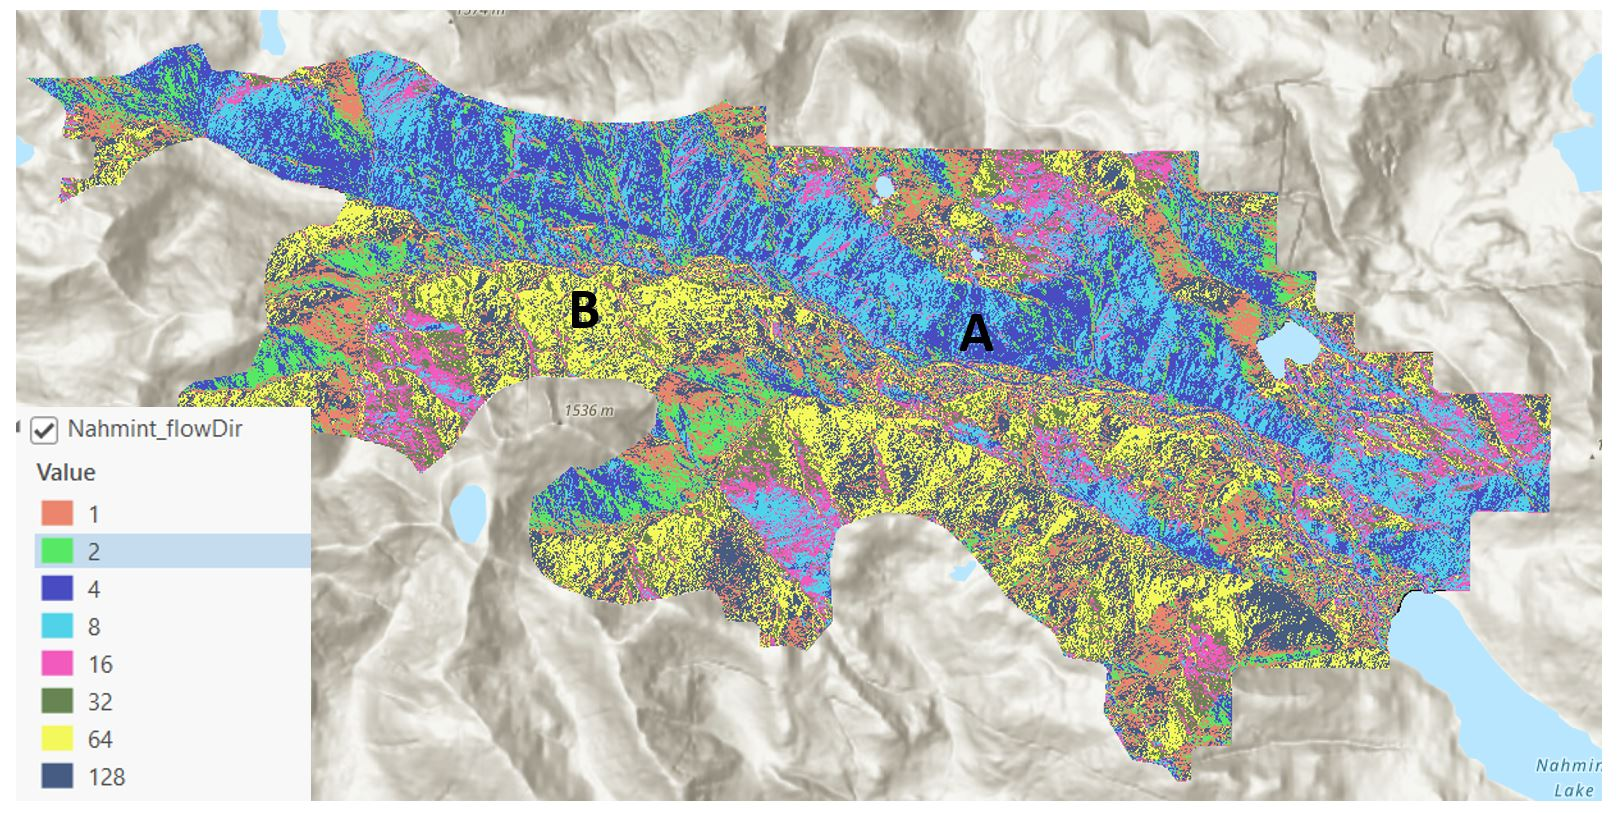
\includegraphics[width=0.75\linewidth]{images/03-flow-direction}

What direction is water flowing at locations A and B? Why do you think this is the case? What topographic features can be seen interpreted from the flow direction raster? Consider these questions when writing your report discussion.

\textbf{Step 3:} We will use the flow direction raster calculated in the last step to calculate flow accumulation, which counts the total number of cells that will flow into a given cell. For example, a cell located at the bottom of the hill will have high flow accumulation and a cell at the top of a hill will not have any flow accumulation. Open the ``Flow Accumulation'' tool and parameterize it as follows:

\begin{itemize}
\tightlist
\item
  Input flow direction raster: \textbf{Nahmint\_FlowDir}
\item
  Output flow accumulation raster: \textbf{FlowAcc}
\item
  Output data type: \textbf{Integer}
\item
  Input flow direction type: \textbf{D8}
\end{itemize}

Leave all other fields blank then run the tool.

\textbf{Step 4:} Next, we will create a raster-based stream network using a threshold in the flow accumulation raster. For example, if the threshold is 100, then only cells with flow accumulation greater than 100 will be counted as a stream. Cells with flow accumulation less than 100 will be set to a background value of 0.

To see how different thresholds impact stream identification, change the symbology of the flow accumulation raster and use the \textbf{Manual Interval} symbology to set two classes. See the example below for a stream network with a flow accumulation threshold of 100 (cells with flow accumulation \textless{} 100 are set to no color).

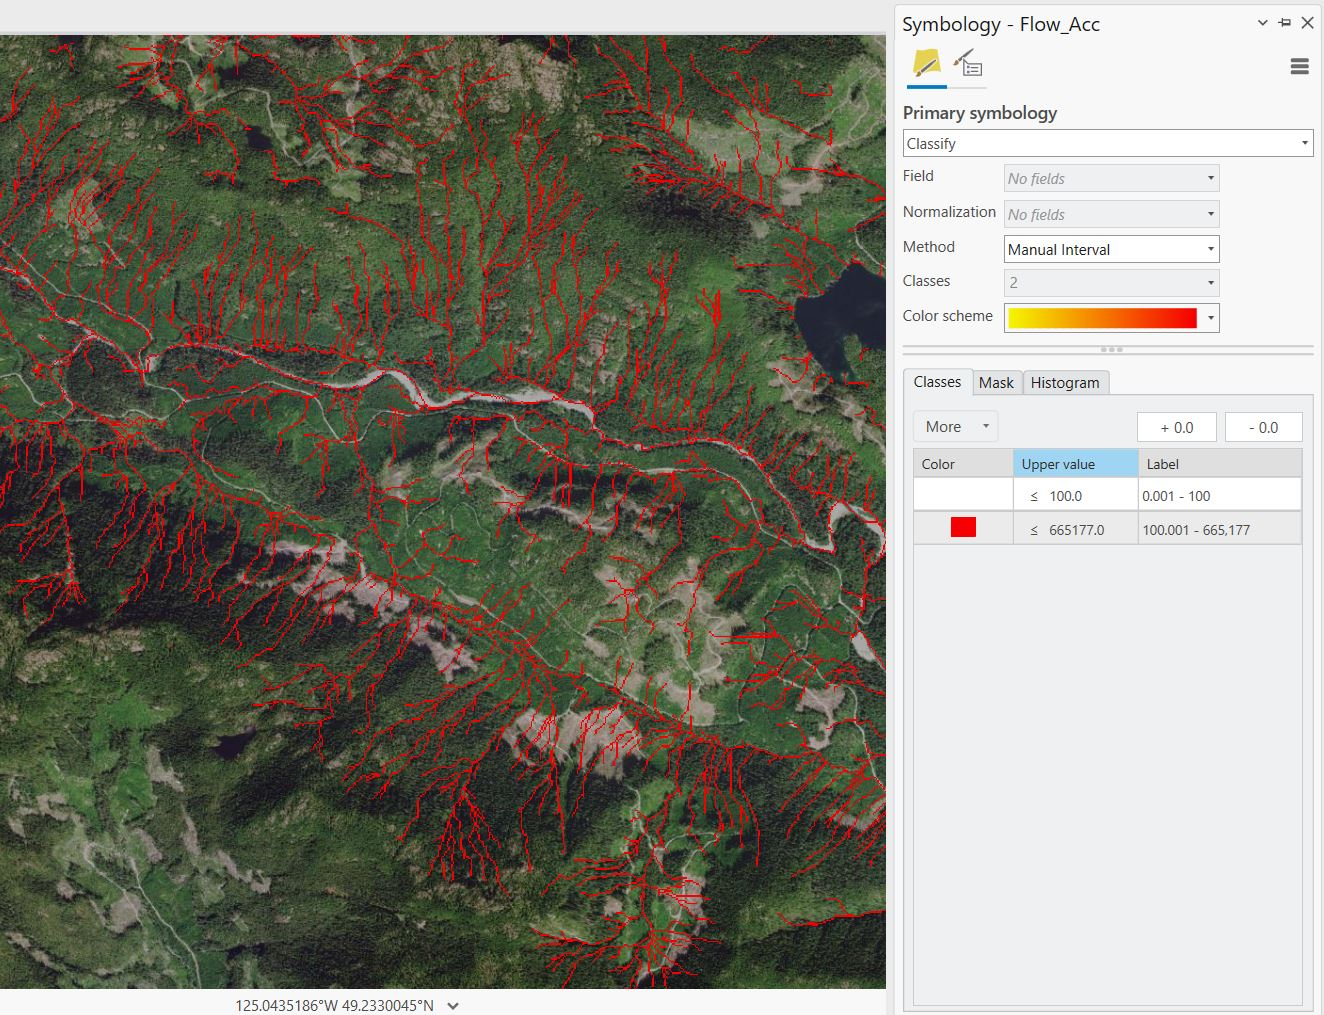
\includegraphics[width=0.75\linewidth]{images/03-streams}

Compare your stream network to the streams visible in the ArcGIS satellite basemap. Experiment with different flow accumulation thresholds. What other features could be misclassified as a stream using this method? Find a threshold that captures streams visible in the basemap, without too many misclassified features.

Once you have selected a threshold, open the ``Reclassify (Spatial Analyst Tools)'' tool.

Use the threshold you have selected as the Start and End values. Set the cells representing streams to a ``New value'' of 1 and all other cells to \texttt{NODATA}. Save the new raster as ``Stream\_reclass''. Include your threshold value in the report Methods section.

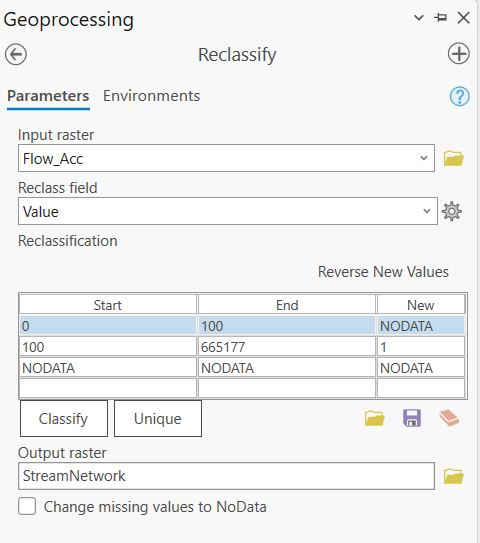
\includegraphics[width=0.75\linewidth]{images/03-reclassify}

Zoom into the reclassified flow accumulation raster to see your stream network.

\textbf{Step 5:} Next, we will assign a stream order to each segment in the stream network. Stream ordering is a system to classify streams based on the number of tributaries (smaller streams) that flow into it. First order streams have no tributaries and higher order streams may have multiple levels of tributaries flowing into it.

Read the following documentation on the Strahler and Shreve methods of stream ordering. \url{https://pro.arcgis.com/en/pro-app/latest/tool-reference/spatial-analyst/how-stream-order-works.htm}

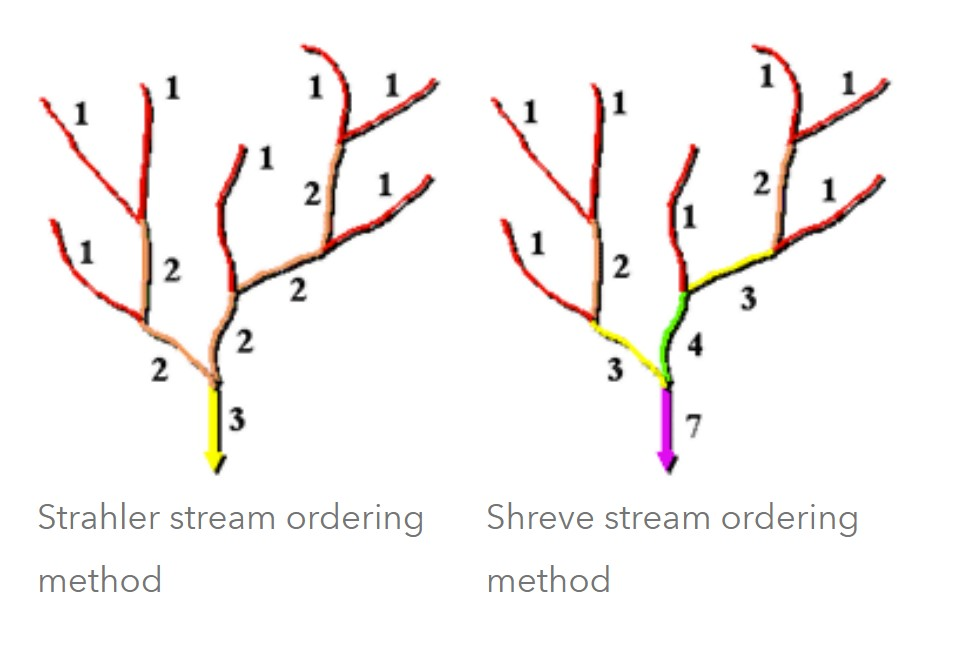
\includegraphics[width=0.75\linewidth]{images/03-stream-order}

Open the ``Stream Order'' tool and parameterize it as follows:

\begin{itemize}
\tightlist
\item
  Input stream raster: \textbf{Stream\_reclass}
\item
  Input flow direction raster: \textbf{Nahmint\_FlowDir}
\item
  Method of stream ordering: \textbf{Strahler}
\item
  Output raster: \textbf{StreamOrder}
\end{itemize}

Zoom in to see the \textbf{StreamOrder} output. The value of each pixel corresponds to the order of each stream segment. Now re-run the tool using the Shreve method and compare the two outputs. Which one produces a more meaningful output and why? In the methods section of your report justify the use of the Stahler method for mapping this stream network.

\textbf{Step 6:} Use the ``Stream to Feature (Spatial Analyst Tools)'' tool to create polyline features representing the ordered stream network. Parameterize the tool as follows:

\begin{itemize}
\tightlist
\item
  Input stream raster: \textbf{StreamOrder}
\item
  Input flow direction raster: \textbf{Nahmint\_FlowDir}
\item
  Output polyline features: \textbf{StreamNetwork\_polyline}
\item
  Simplify polylines: \textbf{Checked}
\end{itemize}

Open the polyline attribute table. The ``grid\_code'' field corresponds to the stream order of the segment. The tool also generates attributes describing the start and end points of each segment and the segment length.

\textbf{Step 7:} Finally, we will assign a unique ID to each stream segment using the ``Stream Link'' tool. Parameterize the tool as follows:

\begin{itemize}
\tightlist
\item
  Input stream raster: \textbf{Stream\_reclass}
\item
  Input flow direction raster: \textbf{Nahmint\_FlowDir}
\item
  Output raster: \textbf{StreamLinks}
\end{itemize}

Zoom in and examine the output.

\begin{center}\rule{0.5\linewidth}{0.5pt}\end{center}

\hypertarget{task-2-extract-stream-characteristics}{%
\section{Task 2: Extract Stream Characteristics}\label{task-2-extract-stream-characteristics}}

In this task we will calculate stream gradient and estimate width for each segment in the network. These metrics will be used to assign a stream class and define the width of the riparian management area.

Gradient is a measure of the streams ``steepness'' and is calculated as:

\[
\frac{EC}{SL}*100
\] \(EC\) is elevation change \(SL\) is stream length

Streams with a gradient \textless20\% are considered ``fish bearing'' in the absence of other field data.

\textbf{Step 1:} First, use the ``Raster Calculator'' tool to multiply the classified flow accumulation layer \textbf{Stream\_reclass} and the \textbf{Nahmint\_DEM} layer. This will give elevation within streams.

\textbf{Step 2:} Open the ``Zonal Statistics'' tool. This tool calculates summary statistics in one raster layer within ``zones'' or groups defined in another layer. This is a very useful tool for many applications! We will use the unique IDs from the \textbf{StreamLinks} layer as ``zones'' to calculate the range in elevation within each stream segment.

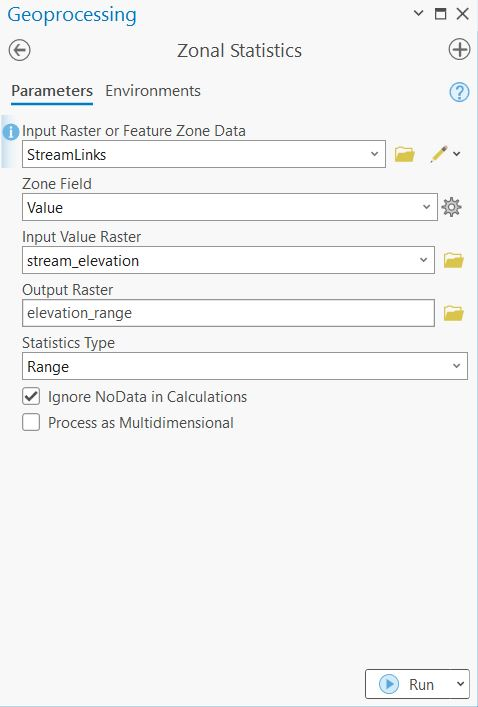
\includegraphics[width=0.75\linewidth]{images/03-zonal-statistics}

The resulting raster shows the gain in elevation within each stream segment.

\textbf{Step 3:} We will convert the elevation change raster to polygon using the ``Raster to Polygon'' tool. Save the output as \textbf{gradient\_polygon}. This step will allow us to perform a spatial join with the vectorized stream network. Open the attribute table and note that some attribute names are the same as the \textbf{StreamNetwork\_polyline}. The attribute ``grid\_code'' represents the elevation gain within each stream segment.

\textbf{Step 4:} Open the ``Spatial Join'' tool and join the \textbf{StreamNetwork\_polyline} with the \textbf{gradient\_polygon}. Parameterize the tool as follows:

\begin{itemize}
\tightlist
\item
  Target Features: StreamNetwork\_polyline
\item
  Join Features: gradient\_polyline
\item
  Output Feature Class: StreamNetwork\_join
\item
  Join operation: Join one to one
\item
  Keep all target features: Checked
\item
  Match Option: Largest Overlap
\item
  Search Radius: 3 Meters
\end{itemize}

Include a rationale for using ``Largest Overlap'' as the ``Match Option'' in the Methods section of your report.

\textbf{Step 5:} Open the attribute table of the output feature class. Notice the duplicated attribute names. The attributes are ordered with the attributes from the Target Feature first and the Join Features second. You may rename and delete unnecessary attributes.

Create a new field called ``Gradient'' and use the ``Calculate Field'' tool to calculate the gradient for each stream segment. Streams with gradient \textless{} 20\% will be considered as ``fish bearing''.

\textbf{Step 6:} Next, we will use the ESRI basemaps to measure stream width for a sample of streams stratified by order. We will use the average stream width per order to approximate the width for all streams in the study area. (For example, if the average width of streams in order 1 is 30 m, all streams in order 1 will be assigned that width).

Stream width is defined using the entire channel width, not just the part with water currently flowing through it. Use the examples below to guide you with your mapping. You should be able to see channels for streams in orders 2-4, but order 1 streams will likely not be visible. We will assign these streams an average width of 1 m.

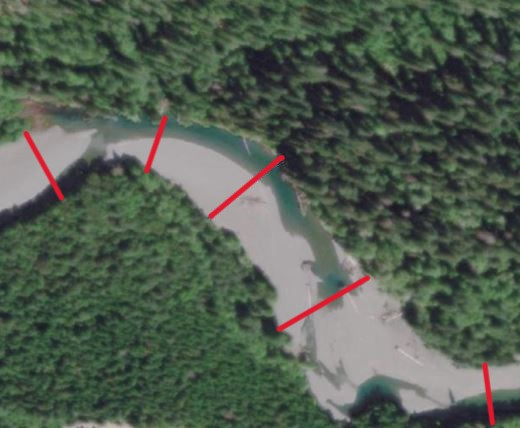
\includegraphics[width=0.75\linewidth]{images/03-s4-stream}

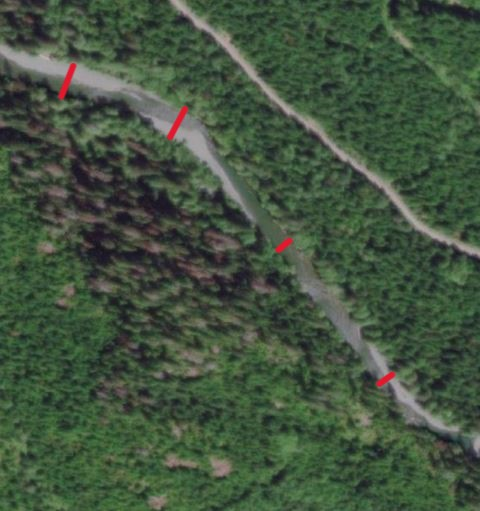
\includegraphics[width=0.75\linewidth]{images/03-s3-stream}

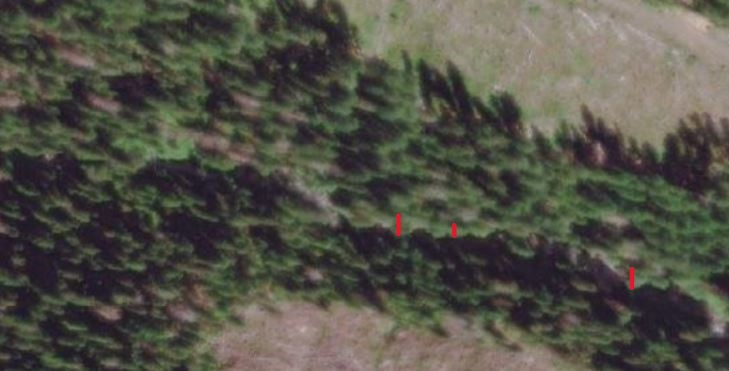
\includegraphics[width=0.75\linewidth]{images/03-s2-stream}

Measure 10-15 stream widths per order using the ``Measure'' tool on your toolbar and record these measurements in an excel document. When you are satisfied with your measurements calculate average width of each stream order. Use the DTM and stream network polyline to help you find some of the smaller order 2 streams.

\textbf{Step 7:} In the \textbf{StreamNetwork\_join} layer, create a new field called ``StreamWidth''. We will use an \texttt{ifelse} statement to conditionally assign values to the stream width attribute depending on stream order. Select the ``StreamWidth'' column in the attribute table and click ``Calculate''. In the ``Calculate Field'' tool, change the ``Expression Type'' to ``Python''.

To use Python in the tool we need to populate two fields. First, the top ``Expression'' field, which should read \texttt{StreamWidth\ =}. This is where we can call a function and define the inputs to the function. Here we have called the function \texttt{reclass} with the ``StreamOrder'' attribute as the input.

Next, in the ``Code Block'' we need to define the \texttt{reclass} function, so that we can use it as part of an expression. Here we will use an \texttt{ifelse} statement to set the values of stream width based on stream order.

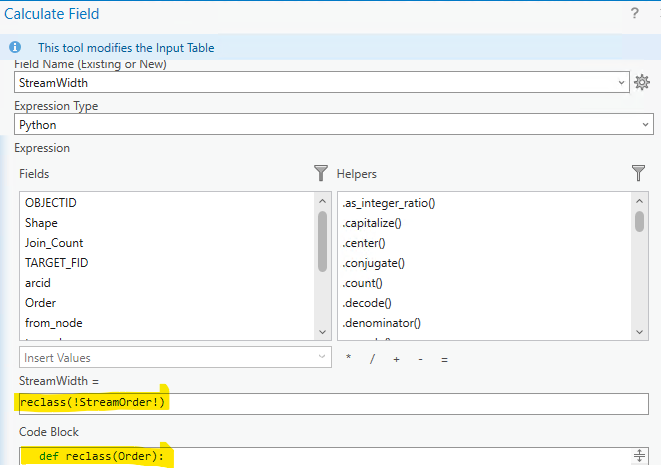
\includegraphics[width=0.75\linewidth]{images/03-python-stream-width}

Modify the following code and paste it into the ``Code Block'' (delete the square brackets before running). Verify the expression using the check button \textgreater{} Apply.

\begin{verbatim}
def reclass(Order):
     if (Order == 1):
          return [average stream width here]
     elif (Order == 2):
          return [average stream width here]
     elif (Order == 3):
          return [average stream width here]
     else:
          return [average stream width here]
\end{verbatim}

If you get an ``Invalid Field'' error it is because the variable in the ``Expression Field'' (between the !!) does not match a field in the attribute table. So make sure to match the name of the appropriate field. You can use the pre-generated Field names to generate your expression to make sure this step works, just double-click on one to add it to your expression.

\begin{center}\rule{0.5\linewidth}{0.5pt}\end{center}

\hypertarget{task-3-mapping-watersheds-and-riparian-management-areas}{%
\section{Task 3: Mapping Watersheds and Riparian Management Areas}\label{task-3-mapping-watersheds-and-riparian-management-areas}}

\textbf{Step 1:} Use the following table to assign a stream class (S1-S6) based on average channel width and fish bearing potential. The Reserve Zone defines the region around the stream where harvest is prohibited and the Management Zone defines the region where limited harvest is permitted. Note that not all stream classes may be present in the dataset.

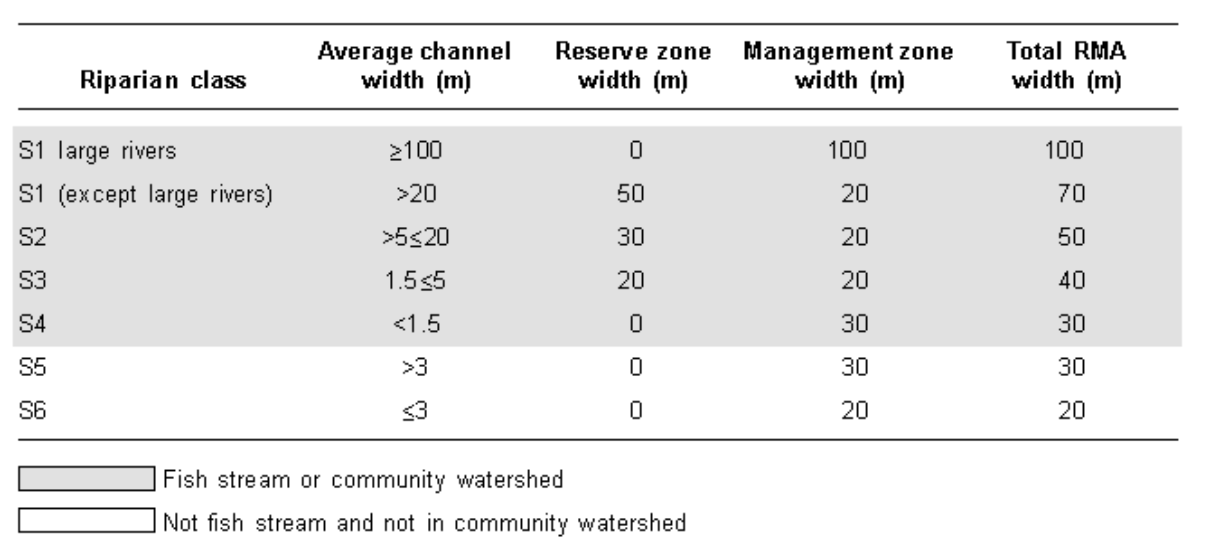
\includegraphics[width=0.75\linewidth]{images/03-stream-class}

In the \textbf{StreamNetwork\_join} layer, create a new attribute called ``Reserve\_BufferDist'' and set the ``Number Format'' to ``Numeric''.

Select the ``Reserve\_BufferDist'' field in the attribute table and open the ``Calculate Field'' tool. Change the ``Expression Type'' to ``Python''.

This time we will combine the \texttt{ifelse} syntax from the previous task with conditional statements to assign buffer distances to each stream class. The example below defines the Reserve Zone buffer distance for the S1 (except large rivers) class using the stream gradient and stream width attributes.

The Reserve Zones and Management Zones are typically measured from the edge of the stream channel, however our streams are represented as lines down the centre of the stream channel. Think of a way to modify the buffer distances in the table to reflect the approximate width of the stream. Include these methods in your report.

Your code should look something like the following (make sure the attribute names in the Expression field match the names in your table!):

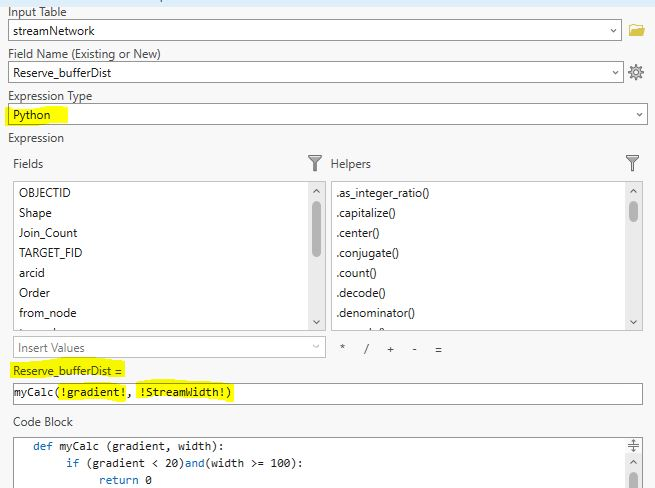
\includegraphics[width=0.75\linewidth]{images/03-stream-network-python}

Use the following template in the ``Code Block'' to calculate the buffer distance for the remaining Reserve Zones (S1-S6). For classes with a width of 0 set the buffer distance to 0.

\begin{verbatim}
def myCalc (gradient, width):
     if (gradient < 20)and(width >= 100):
          return 0
     elif (gradient ...)and(width > ... and width < ...):
     ...
     else:
          return ...
\end{verbatim}

Repeat the same process for the Management Zone widths.

\textbf{Step 2:} Open the ``Buffer'' tool and parameterize it as follows:

\begin{itemize}
\tightlist
\item
  Input Features: \textbf{StreamNetwork\_join}
\item
  Output Feature Class: \textbf{Reserve\_buffer}
\item
  Distance: Use drop-down menu to change to from Linear Unit to \textbf{Field}

  \begin{itemize}
  \tightlist
  \item
    \textbf{Reserve\_BufferDist}
  \end{itemize}
\item
  Side Type: Full
\item
  End type: Round
\item
  Dissolve: Dissolve all output features into a single feature
\end{itemize}

Inspect the output.

Repeat the Buffer step for the Management Zone widths.

\textbf{Step 3:} Next, we will map watersheds. A watershed is an area of land where all the water that falls or flows into it converges to a common outlet, such as a river, lake, or ocean. It is bounded by a drainage divide, which separates water flowing into different watersheds.

The watershed tool uses flow direction and stream links to delineate watershed boundaries. The watershed boundaries will be defined such that water flows into each of the stream links.

Open the ``Watershed'' tool and parameterize it as follows:

\begin{itemize}
\tightlist
\item
  Input D8 flow direction raster: \textbf{Nahmint\_FlowDir}
\item
  Input raster or feature pour point data: \textbf{StreamLinks}
\item
  Output raster: \textbf{Nahmint\_watersheds}
\end{itemize}

The output will be a new raster where the cell values correspond to each unique watershed catchment. You should have something like the following (do not worry if it is not exactly the same):

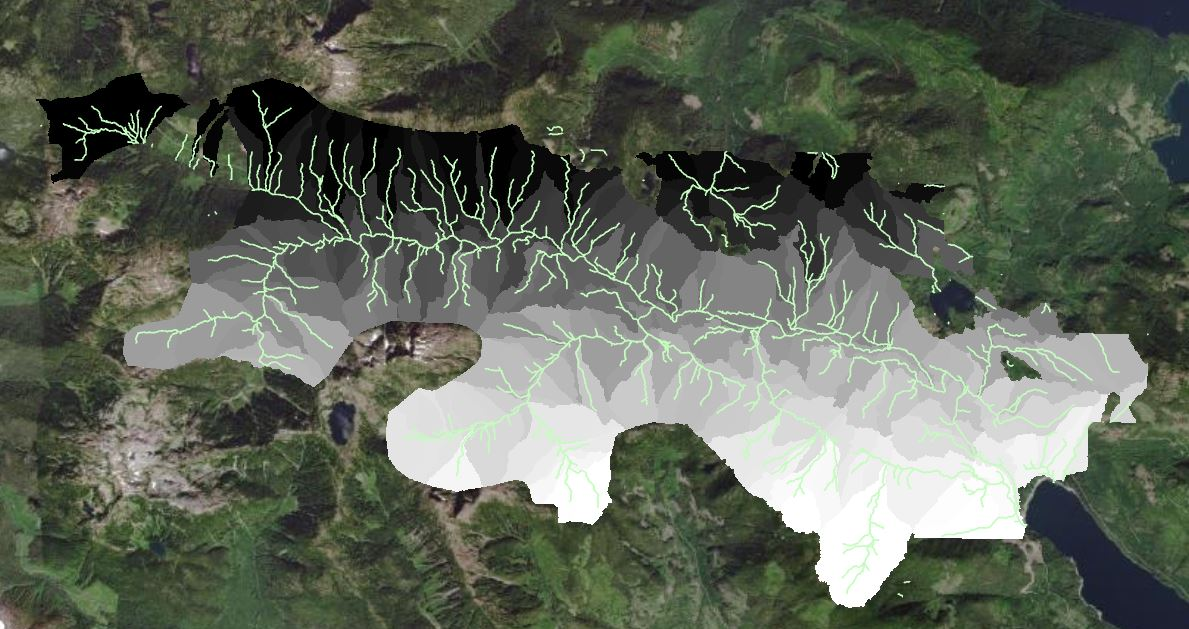
\includegraphics[width=0.75\linewidth]{images/03-map-layers}

\textbf{Step 4:} Finally, we will create contour lines to help interpret the the DTM. Open the ``Contour'' tool and parameterize it as follows:

\begin{itemize}
\tightlist
\item
  Raster: \textbf{Nahmint\_DEM}
\item
  Output features class: \textbf{Nahmint\_contour}
\item
  Contour interval: 100
\item
  Base contour: {[}Set to the lowest elevation in the study area{]}
\item
  Z factor: 1
\item
  Contour type: Contour
\end{itemize}

As your final deliverable create a map with the following elements:

\begin{itemize}
\tightlist
\item
  Watersheds, contour lines
\item
  Stream networks symbolized by stream class
\item
  Example stream network and Riparian Management Areas (Reserve Zone and Management Zone)
\item
  Text showing the total area in the Reserve and Management Zone and the length of the stream network
\item
  Name, date, legend, north arrow, scale bar, title
\end{itemize}

\begin{center}\rule{0.5\linewidth}{0.5pt}\end{center}

\hypertarget{summary-2}{%
\section*{Summary}\label{summary-2}}
\addcontentsline{toc}{section}{Summary}

Here

Return to the \protect\hyperlink{lab3-deliverables}{\textbf{Deliverables}} section to check off everything you need to submit for credit in the course management system.

\hypertarget{machine-learning}{%
\chapter{Machine Learning with Geospatial Data}\label{machine-learning}}

Written by
Claire Armour

\hypertarget{lab-overview-3}{%
\section*{Lab Overview}\label{lab-overview-3}}
\addcontentsline{toc}{section}{Lab Overview}

In this lab, we will be using simple machine learning tools in ArcGIS Pro to predict two variables related to fuel in a post-burn scenario. In Task 1, you will check for spatial autocorrelation in our data and select a subset of input variables which will be most useful in predicting the outcome variables. In Task 2, you will create three different sample datasets using three types of sampling. In Task 3, you will be using a Random Forest classifier to create prediction surfaces for the two variables.

Our area of interest is a large rectangular area in southern British Columbia containing the burn boundary from the 2017 Elephant Hill wildfire. The fire began on July 6th, 2017 and burned 191,865 ha in the south-central Interior region of BC, just northeast of Cache Creek. It was the largest fire by area in the record-breaking 2017 BC wildfire season and was likely started by smoking materials (matches, cigarettes, etc.).

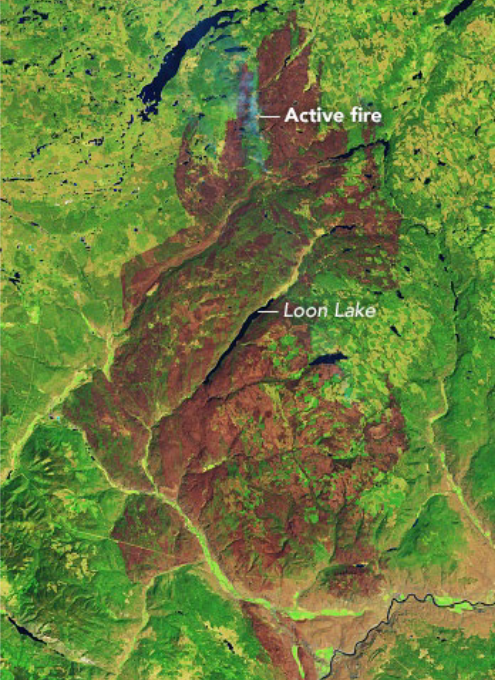
\includegraphics[width=0.75\linewidth]{images/04-elephant-hill-fire}

\begin{center}\rule{0.5\linewidth}{0.5pt}\end{center}

\hypertarget{learning-objectives-3}{%
\section*{Learning Objectives}\label{learning-objectives-3}}
\addcontentsline{toc}{section}{Learning Objectives}

\begin{itemize}
\item
  Compare and contrast sampling designs on machine learning predictions
\item
  Train, test, and predict a continuous variable (crown closure) and a categorical variable (fuel type) using the random forest algorithm
\item
  Evaluate models by interpreting model statistics like R\textsuperscript{2}, AIC, VIF, and confusion matrices
\end{itemize}

\begin{center}\rule{0.5\linewidth}{0.5pt}\end{center}

\hypertarget{lab4-deliverables}{%
\section*{Deliverables}\label{lab4-deliverables}}
\addcontentsline{toc}{section}{Deliverables}

Lab report with the following specification:

6 pages maximum PDF including figures, tables and references (3 points). Single-spaced, 12-point Times New Roman font (1 point). All figures and tables should be properly captioned (1 point).

Introduction should address the following questions and requirements (10 points):

\begin{itemize}
\item
  Conceptually describe how the random forest algorithm works.
\item
  Describe some considerations when selecting different sampling strategies and comment specifically on the sampling strategies that we tested.
\item
  What are the advantages and limitations of using remote sensing data to predict crown closure and fuel types? What about climate data? Terrain data? Why should we use these data for this problem?
\item
  Reference to at least 3 peer review sources.
\end{itemize}

Methods should address the following requirements (10 points):

\begin{itemize}
\item
  Brief study area description and study area map.
\item
  How many fuel types are there in the VRI dataset? Which fuel type has the fewest number of points?
\item
  What is the null hypothesis for the Spatial Autocorrelation tool? Why do we test CROWN\_CLOS for spatial autocorrelation but not FUEL\_TYPE?
\item
  Outline all primary steps included in the lab (no need to include exact ArcGIS Pro tool parameters).
\item
  Justify the use of specific methodological choices indicated in the lab.
\item
  Why do we use ``Closest'' and not ``Intersect'' when doing the spatial join for the FIP data? Consider the geometry of the data. What are the benefits and drawbacks of using each sampling design, both in terms of statistical power and the limits of field data acquisition?
\end{itemize}

Results should address the following questions and requirements (15 points):

\begin{itemize}
\item
  What are the results of the spatial autocorrelation (SA) tool and what do they tell us? Why did we use the K Nearest Neighbours method for this dataset?
\item
  What is the maximum R\textsuperscript{2} value out of all the equations in the results?
\item
  What variables did you choose to include in your model after running exploratory regression? Why did you choose this equation and/or set of variables? Use the statistical terms in the results (R\textsuperscript{2}, p-value, AIC, VIF, variable significance, etc.) to help you explain.
\item
  Map of one of the FUEL\_TYPE rasters and one of the CROWN\_CLOS rasters. Be sure to specify in a caption or title what sampling design / parameter settings you are displaying in each.
\end{itemize}

Discussion should address the following questions and requirements (10 points):

\begin{itemize}
\item
  Display the VRI dataset and observe the distribution of the points across the landscape. What is the main difference between this method and distance-based methods? Why is accounting for spatial autocorrelation in your data important? If you were not limited by the tool inputs, how would you change your sampling design to account for spatial autocorrelation?
\item
  We are constrained by the ArcGIS Pro capabilities and can only use the Exploratory Regression tool with interval or ratio data, i.e., our crown closure variable, so we used the same explanatory variables for both analyses. If you were able to run Exploratory Regression with fuel type, do you think the results would be different? Why or why not?
\item
  Reference to at least 3 peer review sources (can be the same sources as introduction).
\end{itemize}

\begin{center}\rule{0.5\linewidth}{0.5pt}\end{center}

\hypertarget{lab4-data}{%
\section*{Data}\label{lab4-data}}
\addcontentsline{toc}{section}{Data}

All data for this lab are accessible via the UBC PostgreSQL server. Instructions for connecting to the server are given in the tasks below. We will be using data from the \texttt{elephanthill} database.

The data for this lab comes from several different sources, including the Landsat archive and Landsat-derived indices, the ClimateNA program, the Vegetation Resources Inventory (VRI) from the BC Ministry of Forests, and the ASTER (Advanced Spaceborne Thermal Emission and Reflection Radiometer) sensor on the Terra satellite. The VRI is a polygon dataset with hundreds of attributes describing harvest, disturbance, species, volume, etc., for all of BC. The individual rasters and their descriptions are listed on below.

\begin{longtable}[]{@{}
  >{\raggedright\arraybackslash}p{(\columnwidth - 4\tabcolsep) * \real{0.2972}}
  >{\raggedright\arraybackslash}p{(\columnwidth - 4\tabcolsep) * \real{0.6132}}
  >{\raggedright\arraybackslash}p{(\columnwidth - 4\tabcolsep) * \real{0.0849}}@{}}
\toprule\noalign{}
\begin{minipage}[b]{\linewidth}\raggedright
Variable Name
\end{minipage} & \begin{minipage}[b]{\linewidth}\raggedright
Formula or Description
\end{minipage} & \begin{minipage}[b]{\linewidth}\raggedright
Raster Name
\end{minipage} \\
\midrule\noalign{}
\endhead
\bottomrule\noalign{}
\endlastfoot
Elevation & Elevation above vertical datum (meters)

Source: Advanced Spaceborne Thermal Emission and Reflection Radiometer (ASTER) Global Digital Elevation Model Version 3 & ASTER\_DEM \\
Aspect & Azimuth direction, measured clockwise from North (degrees)

Source: ASTER\_DEM & ASTER\_Aspect \\
Slope & Vertical angle from horizontal datum (degrees)

Source: ASTER\_DEM & ASTER\_Slope\_Deg \\
Topographic Radiation Solar Aspect Index (TRASP) & Assigns a value of zero to the north-northeast direction:

\(TRASP=\frac{1-cos(\frac{\pi}{180}(\alpha-30))}{2}\)

Source: ASTER DEM & ASTER\_TRASP \\
Mean Annual Precipitation (MAP) & Millimeters

Source: ClimateNA & CNA\_MAP \\
Mean Annual Temperature (MAT) & Degrees Celsuis

Source: ClimateNA & CNA\_MAT \\
Precipitation as Snow (PAS) & Millimeters

Source: ClimateNA & CNA\_PAS \\
Summer Heat Moisture Index (SHM) & \(\frac{mean\text{ }warmest\text{ }month\text{ }temperature}{\frac{May\text{ }to\text{ }September\text{ }precipitation}{1000} }\)

Source: ClimateNA & CNA\_SHMz \\
Temperature Difference (TD) & \(mean\text{ }warmest\text{ }month-mean\text{ }coldest\text{ }month\)

Source: ClimateNA & CNA\_TD \\
Normalized Difference Vegetation Index (NDVI) & \(NDVI=\frac{NIR-Red}{NIR+Red}\)

Source: Landsat & Landsat\_NDVI \\
Normalized Difference Burn Ratio (NBR) & \(NBR=\frac{NIR-SWIR}{NIR+SWIR}\)

Source: Landsat & Landsat\_NBR \\
Tasseled Cap Brightness (TCB), Wetness (TCW), Greeness (TCG) & \(TCB=Band1*coeff1\)

\(TCW=Band1*coeff1\)

\(TCG=Band1*coeff1\)

Source: Landsat & Landsat\_TCB

Landsat\_TCW

Landsat\_TCG \\
\end{longtable}

The data have been processed ahead of time so that you may focus more on machine learning and sampling design. If you wanted to replicate this workflow in another area of your work, here are the steps we used:

\begin{enumerate}
\def\labelenumi{\arabic{enumi}.}
\tightlist
\item
  Obtained the ClimateNA, ASTER, VRI, and Landsat data appropriate to the study area/time period.
\item
  Projected all the data to NAD 1983 BC Environmental Albers geographic coordinate system and clipped it to the study area boundary.
\item
  Calculated Normalized Difference Vegetation Index (NDVI), Normalized Burn Ratio (NBR), and Tasseled Cap Wetness (TCW), Greenness (TCG), and Brightness (TCB) using the appropriate bands from the Landsat image.
\item
  Normalized all the rasters (including the indices) using the standard formula where x is a pixel value, mu is the mean pixel value of the raster, and omega is the standard deviation of the raster.
\item
  Cleaned the VRI data by removing all unneeded fields and records with \texttt{\textless{}Null\textgreater{}} values for our variables of interest.
\item
  Used the ``Extract Multi Values to Points'' tool to extract the values of all our rasters to our VRI point feature class (similar to a Spatial Join). Checked for \texttt{\textless{}Null\textgreater{}} or values again and removed.
\end{enumerate}

\begin{center}\rule{0.5\linewidth}{0.5pt}\end{center}

\hypertarget{task-1-exploratory-regression-in-arcgis-pro}{%
\section*{Task 1: Exploratory Regression in ArcGIS Pro}\label{task-1-exploratory-regression-in-arcgis-pro}}
\addcontentsline{toc}{section}{Task 1: Exploratory Regression in ArcGIS Pro}

\textbf{Step 1:} Start ArcGIS Pro and create a new project with a map template.

\textbf{Step 2:} Connect to the UBC PostgreSQL database and import all of the data from the \texttt{elephanthill} database into your project geodatabase. This should include 14 rasters, the Vegetation Resource Inventory (VRI) point feature class, and the Elephant Hill (EH) boundary. Open the attribute table for the VRI and see what fields are there. We will not be using the EH boundary for any analysis but it is interesting to see where the fire took place. It truly is a megafire!

\textbf{Step 3:} Set the ``Primary symbology'' on the VRI feature class to ``Graduated Colors'' and choose ``CROWN\_CLOS'' as the field to display. Take a look at the results and then set ``FUEL\_TYPE'' as the field to display. These are the two variables we will be predicting -- crown closure (also known as canopy cover) and fuel type. CROWN\_CLOS is continuous and FUEL\_TYPE is categorical. You will notice there are quite a few VRI points (over 84,000), so save your laptop the extra rendering work and turn off this layer unless you are actively looking at it.

\textbf{Step 4:} Open the ``Spatial Autocorrelation (Global Moran's I)'' tool. Use the VRI feature class as the input and set the input field to ``CROWN\_CLOS''. Change the ``Conceptualization of Spatial Relationships'' parameter to ``K Nearest Neighbours'' and set the ``Number of Neighbors'' to ``20''. Check the box that says ``Generate Report''. Leave the rest of the tool parameters with the default values and run the tool. Observe the results by viewing the generated report (found in your default folder/geodatabase) or by selecting ``View Details''.

\textbf{HINT: Due to the constraint of completing this lab in ArcGIS Pro, we are unable adjust our sampling parameters to account for spatial autocorrelation. Fortunately, this is a learning exercise, so you will get to discuss this conundrum in your report!}

Next, we are going to use Exploratory Regression to determine which of our rasters will be most effective in predicting our variables of interest.

\textbf{Step 5:} Open the ``Exploratory Regression'' tool and set the VRI feature class as your ``Input Features''. Select ``CROWN\_CLOS'' as your ``Dependent Variable''. Remember that as part of the pre-processing, all raster data were extracted at the VRI points. Select the fields corresponding to the rasters in the VRI feature class as your ``Candidate Explanatory Variables''. Leave out the original Landsat bands. Save the ``Output Report File'' as ``regression\_results.txt''. This will create a text file in your default folder with the results of the tool, which can also be viewed under ``View Details''. Leave the rest of the tool parameters as the default values and run the tool.

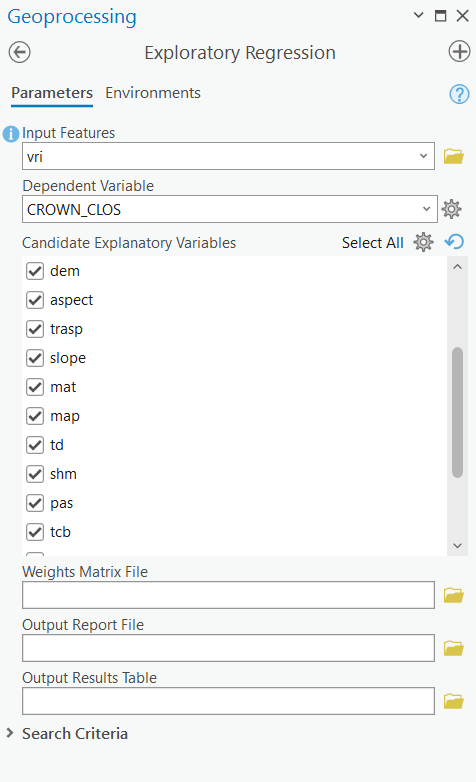
\includegraphics[width=0.75\linewidth]{images/04-exploratory-regression}

\textbf{Step 6:} Select the equation you think will work best. Remember to look at all the different measures of model ``goodness'' (R\textsuperscript{2}, AIC, VIF, multicollinearity, etc.). Our variable rasters fall into three categories: terrain, spectral, and climate. Our final equation should include at least one variable from each category. Write down the variables from your chosen equation somewhere as you will have to re-enter them later.

\begin{center}\rule{0.5\linewidth}{0.5pt}\end{center}

\hypertarget{task-2-sampling-for-training-datasets}{%
\section*{Task 2: Sampling for Training Datasets}\label{task-2-sampling-for-training-datasets}}
\addcontentsline{toc}{section}{Task 2: Sampling for Training Datasets}

As noted earlier, the VRI feature class is enormous, and it is an outlier regarding the typical number of field samples we would have to work with. Training on 80,000+ points would also require an equally vast amount of computing power, so we are going to cull this dataset into a more manageable 500 points. This also gives us the opportunity to create and compare sampling designs: random sampling, stratified random sampling, and fixed interval point sampling.

\textbf{Step 1:} First, we will make a randomly sampled dataset. Open the tool ``Subset Features'' and set the VRI feature class as the ``Input features''. Name your ``Output training feature class'' as ``random\_sample'' and leave the ``Output test feature class'' blank (this option creates a second feature class for testing but we do not need that). Change the ``Subset size units'' to ``ABSOLUTE\_VALUE'', as we want a specific number of points and not a percentage of the dataset. Set the ``Size of training feature subset'' to 500 and run the tool. View the output on your map.

\textbf{Step 2:} Next, we want to make a stratified randomly sampled dataset. There are four major categories of fuel types in our dataset and their distribution is highly uneven. This design will ensure the rarest class is as equally represented as the most abundant class in our sample. As there are four categories (fire, non-vegetated, vegetated non-forest, and forest), we will sample 125 points from each. The list below tells you what fuel type codes correspond to each category:

\begin{itemize}
\tightlist
\item
  Fire -- ``N-fire''
\item
  Non-vegetated -- ``N''
\item
  Vegetated non-forest -- all fuel types starting with ``S'' or ``O'' (as in octopus).
\item
  Forest -- all fuel types starting with ``M'', ``C'', or ``D''.
\end{itemize}

Open the attribute table for the VRI dataset, right-click on the ``FUEL\_TYPE'' field, and select ``Summarize''. Set the ``Field'' to ``FUEL\_TYPE'' and the ``Statistic Type'' to ``Unique''. Leave ``Case Field'' as is and select ``OK''. Inspect the output statistics table in your Contents Pane.

\textbf{Step 3:} Using the ``Select by Attribute'' tool, select all the features in the VRI feature class that have a ``FUEL\_TYPE'' of ``N-fire''. Right-click the feature class, select ``Selection'', then select ``Make Layer from Selected Features''.

\textbf{Step 4:} Using the ``Subset Features'' tool again, set your parameters to subset 125 points from the layer you created in the previous step. Name the output ``fire\_sub\_sample'' and check the attribute table to make sure all of the records in this feature class have a fuel type of ``N-fire''.

\textbf{Step 5:} Clear your selection. Right-click ``VRI'', select ``Selection'', then select ``Clear Selection'' and repeat steps 3 and 4 for the remaining three categories. Give the outputs logical names and clear your selection/delete the selection layer between each.

\textbf{HINT: Use the ``begins with'' operator to select all fields with a certain letter rather than ``is'', but beware that both ``N'' and ``N-fire'' begin with the same letter.}

Double-check that your sub-samples have the correct number and fuel types in them.

\textbf{Step 6:} Using the ``Merge'' tool, combine your four sub-sample data sets and call the output ``stratified\_sample''. This sample should have 500 points.

\textbf{Step 7:} To make the fixed interval point (FIP) sampled dataset, we will create a regularly spaced grid from which to sample our points by creating a fishnet of polygons, converting those polygons into centroid points, and then sampling the closest VRI point to our fishnet points. Open the ``Create Fishnet'' tool and name your ``Output Feature Class'' ``fishnet''. Set your ``Template Extent'' to the VRI point feature class. The coordinates should match what you see in the screenshot below. Set the ``Number of Rows'' to 20 and the ``Number of Columns'' to 25. This divides the extent into 20x25 (500!) identical segments. Change the ``Geometry'' to ``Polygon'' and run the tool. Your output feature class should look like the grid below.

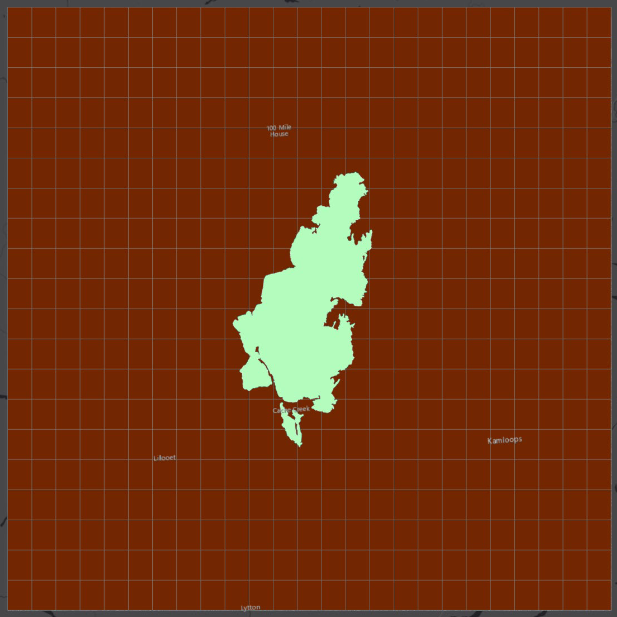
\includegraphics[width=0.75\linewidth]{images/04-elephant-hill-fishnet}

\textbf{Step 8:} Open the ``Feature to Point'' tool and use your fishnet from the previous step as the input. The default of this tool when used with polygon geometry is to place a point at the center of each polygon. If you overlay your new point feature class onto your fishnet, it should look like the screenshot below.

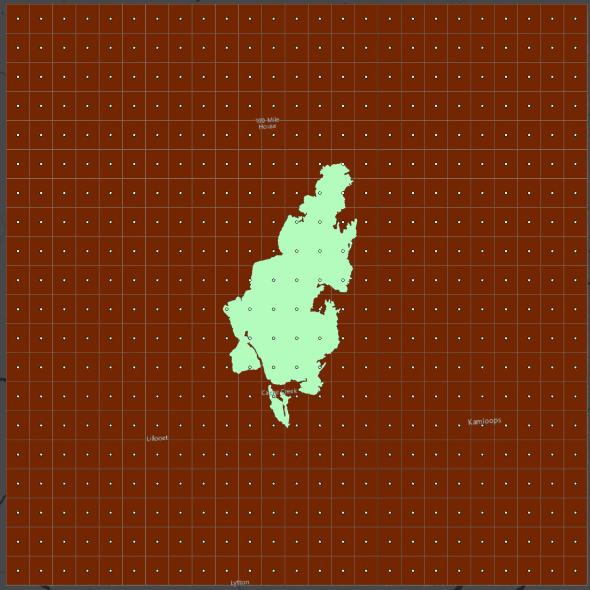
\includegraphics[width=0.75\linewidth]{images/04-elephant-hill-fishnet-points}

\textbf{Step 9:} We have a nice lattice of points across our study area, and we have a point feature class to sample from, but we need to put them together. Open the ``Spatial Join'' tool and set your fishnet points (not polygons!) as the ``Target Features'' and your VRI point feature class as the ``Join Features''. Set ``Closest'' as the ``Match Option''. This will find the closest VRI point to the fishnet and join it to the table. The ``Join Operation'' should be ``Join one to one'' and your ``Search Radius'' can be left blank. Name your ``Output Feature Class'' ``FIP\_sample'' and run the tool.

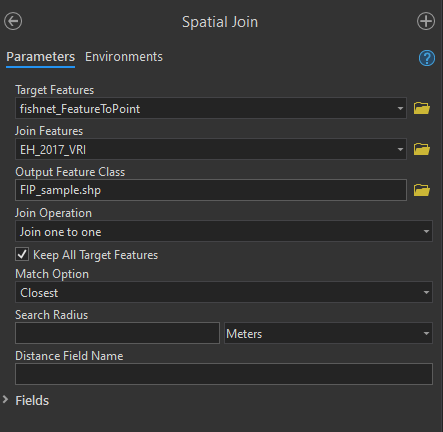
\includegraphics[width=0.75\linewidth]{images/04-spatial-join}

You now have three sampling sets to try your machine learning with!

\begin{center}\rule{0.5\linewidth}{0.5pt}\end{center}

\hypertarget{task-3-forest-based-classification}{%
\section*{Task 3: Forest-Based Classification}\label{task-3-forest-based-classification}}
\addcontentsline{toc}{section}{Task 3: Forest-Based Classification}

Our last task will be using the ``Forest-based Classification and Regression'' tool to run our machine learning. ESRI provides a helpful overview of the tool \href{https://pro.arcgis.com/en/pro-app/latest/tool-reference/spatial-statistics/how-forest-works.htm}{here}. We will be running it a total of nine times (three with FUEL\_TYPE, six with CROWN\_CLOS) and it can be slow, so please be patient and leave yourself lots of time.

\textbf{Step 1:} Open the ``Forest-based Classification and Regression'' tool. When you search for the tool, check that it is from the ``Spatial Statistics'' toolbox and NOT the ``GeoAnalytics Desktop'' toolbox as they have different inputs. Parameterize the tool as follows:

\begin{itemize}
\tightlist
\item
  \textbf{Prediction Type:} Predict to Raster
\item
  \textbf{Input Training Features:} random\_sample
\item
  \textbf{Variable to Predict:} FUEL\_TYPE
\item
  \textbf{Treat Variable as Categorical:} check this box (our variable is categorical)
\item
  \textbf{Explanatory Training Rasters:} drag in your variable rasters that you selected from Exploratory Regression in Task 1. The screenshot below shows one potential raster but you should have a maximum of 5.
\item
  \textbf{Output Prediction Surface:} random\_output\_FT (CC for CROWN\_CLOS, FT for FUEL\_TYPE)
\item
  \textbf{Match Explanatory Rasters:} they should already match, but double check the prediction rasters are matched to the correct field in the training data.
\item
  \textbf{Additional Outputs \textgreater{} Output Classification Performance Table (Confusion Matrix):} random\_matrix\_FT
\item
  \textbf{Validation Options \textgreater{} Training Data Excluded for Validation:} set to 30\%
\item
  \textbf{Validation Options \textgreater{} Number of Runs for Validation:} set to 2
\end{itemize}

Leave all other parameters as the default value or blank. Run the tool. You may get a warning about low numbers of certain fuel types -- ignore it (for now\ldots). When the tool finishes, click ``View Details'' and copy/paste the info under ``Messages'' into a text file. This is where you can find the regression statistics (R\textsuperscript{2}, RMSE, etc) for the training and validation data for your report.

\textbf{Step 2:} Run the tool again, but this time use ``stratified\_sample'' as your ``Input Training Features''. Change the name of your outputs accordingly, but keep everything else the same. When this is finished, run the tool a third time with ``FIP\_sample'' as the input. Remember to keep your regression results in a text file. If you do forget, just go to ``History'' under the ``Analysis'' tab and hover over the tool.

\textbf{HINT: Under the ``Analysis'' tab, view your tool ``History''. Double-click the ``Forest-based Classification and Regression'' tool and it will pop up in your geoprocessing pane with the same inputs and settings you used for that particular run -- this way, you can just edit the inputs that are changing between runs rather than having to reenter the settings each time.}

For CROWN\_CLOS, instead of changing the sampling design, we are going to experiment with different parameter settings on the tool for a total of 6 runs (three different parameters, two settings each).

\textbf{Step 3:} Open the ``Forest-based Classification and Regression'' tool again and set these inputs which will act as our control:

\begin{itemize}
\tightlist
\item
  \textbf{Prediction Type:} Predict to Raster
\item
  \textbf{Input Training Features:} random\_sample
\item
  \textbf{Variable to Predict:} CROWN\_CLOS
\item
  \textbf{Treat Variable as Categorical:} Uncheck this box (our variable is continuous interval)
\item
  \textbf{Explanatory Training Rasters:} same as FUEL\_TYPE
\item
  \textbf{Output Prediction Surface:} control\_output\_CC
\item
  \textbf{Match Explanatory Rasters:} same as FUEL\_TYPE
\item
  \textbf{Advanced Forest Options \textgreater{} Number of Trees:} set to 50
\item
  \textbf{Validation Options \textgreater{} Training Data Excluded for Validation:} set to 30\%
\end{itemize}

Leave all other parameters as the default value or blank. Run the tool. When it is finished, click ``View Details'' and copy/paste the info under ``Messages'' into your text file.

\textbf{Step 4:} We are going to run the ``Forest-based Classification and Regression'' tool six more times. For each time, the inputs should be identical to those in Step 3 except for a single parameter which we will change each time:

\begin{itemize}
\tightlist
\item
  \textbf{Run 1 of 6:} Change Advanced Forest Options \textgreater{} Maximum Tree Depth to 5. Name the output ``depth\_5\_output\_CC''
\item
  \textbf{Run 2 of 6:} Change Advanced Forest Options \textgreater{} Maximum Tree Depth to 15. Name the output ``depth\_15\_output\_CC''
\item
  \textbf{Run 3 of 6:} Change Advanced Forest Options \textgreater{} Number of Randomly Sampled Variables to 1. Name the output ``var\_1\_output\_CC''
\item
  \textbf{Run 4 of 6:} Change Advanced Forest Options \textgreater{} Number of Randomly Sampled Variables to 2. Name the output ``var\_2\_output\_CC''
\item
  \textbf{Run 5 of 6:} Change Validation Options \textgreater{} Number of Runs for Validation to 2. Name the output ``runs\_2\_output\_CC''
\item
  \textbf{Run 6 of 6:} Change Validation Options \textgreater{} Number of Runs for Validation to 10. Name the output ``runs\_10\_output\_CC''
\end{itemize}

\textbf{DO NOT FORGET TO CHANGE YOUR OTHER SETTINGS BACK TO THE DEFAULT BETWEEN EACH RUN.} If you want to be extra sure, open the ``Forest-based Classification and Regression'' tool from ``History'' where you ran your CROWN\_CLOS control (which has all the defaults) and do each run from there. You can check your inputs under ``View Details'' if you want to double-check.

When you are finished you should have 10 output rasters, 3 output confusion matrices, and 7 text files with your regression results.

\textbf{Step 5:} View all of your new rasters in your map and inspect the results. Symbolize them in a logical manner.

Your output rasters for FUEL\_TYPE may be numbers, even though the variable was a string! If your fuel type prediction rasters show numbers, do the following: on each of your sample feature classes, open the attribute table and summarize the unique values in the FUEL\_TYPE field using the same method as Task 2 Step 2. The OID in the summary table and the value in your corresponding output raster refer to the same fuel type, e.g., 0 is C-2, 1 is C-3, etc, as seen to the left. Change the labels for the legend in raster Symbology to the fuel type instead of the number when you make the map.

\begin{center}\rule{0.5\linewidth}{0.5pt}\end{center}

\hypertarget{summary-3}{%
\section*{Summary}\label{summary-3}}
\addcontentsline{toc}{section}{Summary}

There are many things to consider when undertaking machine learning with geospatial data. Although we only practiced with the random forest algorithm, many of these considerations are important for other methods as well. Machine learning algorithms work well for large datasets where you can randomly apportion testing, training and validation datasets. When applying these algorithms to spatial data, we often need to consider data density in the spatial and sometimes temporal domains. Interrogating spatial and temporal autocorrelation can help to identify the appropriate sampling strategy for your problem. As you learned in this lab, even the type of variable that you are predicting (continuous vs discrete) can require completely different methods for data handling, testing, and validation. Keep in mind that most of the data pre-processing was removed from the lab (see \protect\hyperlink{lab4-data}{Data}) so that you could focus on the analysis, though these efforts remain some of the most time-consuming to ensure a successful analysis.

Return to the \protect\hyperlink{lab4-deliverables}{\textbf{Deliverables}} section to check off everything you need to submit for credit in the course management system

\hypertarget{geographically-weighted-regression}{%
\chapter{Analyzing Green Equity Using Geographically Weighted Regression}\label{geographically-weighted-regression}}

Written by
Paul Pickell

\hypertarget{lab-overview-4}{%
\section*{Lab Overview}\label{lab-overview-4}}
\addcontentsline{toc}{section}{Lab Overview}

In this lab, you will be exploring a few different statistical approaches to modelling geographic data, including geographically weighted regression (GWR). GWR is the spatial extension of aspatial regression analysis and much more. Traditional regression analysis assumes that global statistics adequately describe local relationships that might exist in the data. For example, consider looking at the relationship between housing prices and the floor space, lot size, etc., of houses in the city of Vancouver. While we could develop a `global' model that adequately describes the relationship between those variables, knowing what you do about housing prices in the city of Vancouver (e.g., that a house of similar dimensions, age, lot size, etc., in the east side of Vancouver will sell for hundreds of thousands of dollars less than an identical house in the west side of Vancouver), the utility of such a model when looking at neighborhood-level housing issues would be very doubtful. Nonetheless, for decades such models, such as hedonic models, have been normalized in real estate research.

Similarly, consider studying the relationship between rates of crime or diseases to environmental conditions, local conditions can be much more important than any global relationship that might be discovered via a traditional aspatial statistical approach. Using polygon or point data, GWR allows us to explore the local relationships amongst a set of variables and examine the results spatially using ArcGIS Pro. It should be noted that in R you can find more sophisticated approaches to GWR than what is provided by ArcGIS Pro.

In this lab, you will explore the equity of green space for the city of Vancouver using Landsat imagery and demographic data from the 2021 Canadian census.

Why is access to green spaces so important? Human well-being, including physical and psychological well-being increase when residents are exposed to green space and urban forests. In addition, ecosystem services provided from green spaces include improved air quality, urban heat island mitigation, and opportunities for recreation. Yet, there is unequal access to green spaces across urban landscapes. The distribution of green space is often disproportionately present in affluent communities. So, you will test the hypothesis that there is less green space in marginalized communities. We cannot infer any causal relationships, but we can examine the relationship between the location of green spaces and demographic variables.

Vancouver is the most populous city in British Columbia, Canada with a population of 662,248 in 2021. Vancouver is an ideal study site because of the city's high level of heterogeneity among its demographic and green space structure.

\begin{center}\rule{0.5\linewidth}{0.5pt}\end{center}

\hypertarget{learning-objectives-4}{%
\section*{Learning Objectives}\label{learning-objectives-4}}
\addcontentsline{toc}{section}{Learning Objectives}

\begin{itemize}
\item
  Apply advanced SQL and PostGIS functions to a relational database to prepare high-dimensional census data for analysis
\item
  Calculate a vegetation index from Landsat imagery and report summary statistics over census dissemination areas
\item
  Evaluate different models and defend your model selection
\item
  Interpret charts and statistics of ordinary least squares and geographically weighted regression
\item
  Map geographically weighted regression results and interpret and defend your conclusions
\end{itemize}

\begin{center}\rule{0.5\linewidth}{0.5pt}\end{center}

\hypertarget{lab5-deliverables}{%
\section*{Deliverables}\label{lab5-deliverables}}
\addcontentsline{toc}{section}{Deliverables}

Lab report with the following specification:

6 pages maximum PDF including figures, tables and references (3 points). Single-spaced, 12-point Times New Roman font (1 point). All figures and tables should be properly captioned (1 point).

Introduction should address the following questions and requirements (10 points):

\begin{itemize}
\item
  Describe geographically weighted regression and compare it with ordinary least squares.
\item
  Reference to at least 3 peer review sources.
\end{itemize}

Methods should address the following requirements (10 points):

\begin{itemize}
\item
  Brief study area description and study area map.
\item
  Describe the qualities of the census data and the Landsat image.
\item
  Outline all primary steps included in the lab (no need to include exact ArcGIS Pro tool parameters).
\item
  How did you evaluate your models and select your final model? Report any relevant statistics that you used in your judgement.
\item
  Why did you select the 10 characteristics that you choose in Task 3?
\item
  Justify the use of specific methodological choices indicated in the lab.
\end{itemize}

Results should address the following questions and requirements (15 points):

\begin{itemize}
\item
  A table with the ordinary least squares and geographically weighted regression results for the model that used your 10 characteristics.
\item
  Describe all of the terms, coefficients, and explanatory variables of your selected GWR model.
\item
  Justify your choice of a final set of independent variables for your GWR model.
\item
  Compare and contrast the different NDVI statistics. Which statistic had the best model? What evidence do you have for that conclusion? Why do you think that relationship was the strongest?
\item
  Interpret one of your independent variables in one of your three NDVI statistics using the Std.Error and Coefficient map. What spatial patterns do you see? What do you think could be influencing this relationship?
\item
  Maps illustrating the standardized residuals and local R\^{}\{2\} for each of your three different NDVI statistics.
\end{itemize}

Discussion should address the following questions and requirements (10 points):

\begin{itemize}
\item
  What other factors (spatial or aspatial) might be contributing or confounding your analysis? In other words, what other data sources might you add/calculate or what methods might you change to improve your results?
\item
  What can you conclude about green equity among dissemnination areas in Vancouver?
\item
  What are your final recommendations to city council about green equity in Vancouver?
\item
  Reference to at least 3 peer review sources (can be the same sources as introduction).
\end{itemize}

\begin{center}\rule{0.5\linewidth}{0.5pt}\end{center}

\hypertarget{data}{%
\section*{Data}\label{data}}
\addcontentsline{toc}{section}{Data}

All data for this lab are accessible via the UBC PostgreSQL server. Instructions for connecting to the server are given in the tasks below. We will be using data from the \texttt{greenequity} database.

Statistics Canada. 2022. Census Profile. 2021 Census. Statistics Canada Catalogue no. 98-316-X2021001. Ottawa. Released December 15, 2022. \url{https://www12.statcan.gc.ca/census-recensement/2021/dp-pd/prof/index.cfm?Lang=E}

We are using only a small subset of the national 2021 census data set for British Columbia: ``Canada, provinces, territories, census divisions (CDs), census subdivisions (CSDs) and dissemination areas (DAs) - British Columbia only'' (Statistics Canada Catalogue no. 98-401-X2021006).

The Statistics Canada 2021 spatial boundary files are maintained separately and available for download from here: \url{https://www12.statcan.gc.ca/census-recensement/2021/geo/sip-pis/boundary-limites/index2021-eng.cfm?year=21}

The spatial data from Statistics Canada that we will be using:

\begin{longtable}[]{@{}ll@{}}
\toprule\noalign{}
Layer Name & Description \\
\midrule\noalign{}
\endhead
\bottomrule\noalign{}
\endlastfoot
lcsd000b21a\_e & Census subdivisions \\
lda\_000b21a\_e & Dissemination areas \\
\end{longtable}

If you are a student at UBC, these data have already been prepared and loaded into the UBC PostgreSQL server, so there is no need to download anything. The links above are only for reference.

Metadata for the 2021 spatial boundary files can be found here: \url{https://www150.statcan.gc.ca/n1/pub/92-160-g/92-160-g2021002-eng.htm}

The Dictionary for Census of Population 2021 can be found here: \url{https://www12.statcan.gc.ca/census-recensement/2021/ref/dict/index-eng.cfm}

\begin{center}\rule{0.5\linewidth}{0.5pt}\end{center}

\hypertarget{task-1-prepare-census-data}{%
\section*{Task 1: Prepare census data}\label{task-1-prepare-census-data}}
\addcontentsline{toc}{section}{Task 1: Prepare census data}

Statistics Canada census data are distributed in tables, which are great for working with in a relational database like PostgreSQL. These data can be particularly challenging to work with because they span multiple geographical hierarchies (e.g., national, provincial, municipal, etc.), multiple dates (the Canadian census occurs every 5 years), many demographic dimensions (e.g., population, age, education, language, etc.), and there are an enormous amount of enumerated areas.

The smallest geographic unit that census data are enumerated over are known as Dissemination Areas (DA). Statistics Canada gives the definition:

\begin{quote}
A dissemination area (DA) is a small, relatively stable geographic unit composed of one or more adjacent dissemination blocks with an average population of 400 to 700 persons based on data from the previous Census of Population Program. It is the smallest standard geographic area for which all census data are disseminated. DAs cover all the territory of Canada.
\end{quote}

As of the 2021 Canadian census, there are 57,936 unique Dissemination Areas. Each Dissemination Area is described by 2,631 unique characteristics (total population, age, education, language, etc.). That is a whopping 152 million values for describing Canadians! Lucky for us, we will be working with DAs for Vancouver, British Columbia and only a handful of characteristics.

To make this a realistic exercise, we will be working with the raw Statistics Canada table for British Columbia and the national set of dissemination areas, which have been loaded into the UBC PostgreSQL server. These data are also publicly available if you want to replicate the lab on your own (see \protect\hyperlink{data}{Data} section)

\textbf{Step 1:} Open QGIS and connect to the \texttt{greenequity} database on the UBC PostgreSQL server using the credential that you have been provided. You might be tempted to add the layers \textbf{lda\_000b21a\_e} and \textbf{lcsd000b21a\_e} to your map. You can do this, but it will probably slow down your computer as you are requesting all 57,936 dissemination areas and 5,161 census subdivisions from the server, respectively. Instead, we will use some PostGIS magic to filter on the server side before making our request for only the Vancouver DAs to our QGIS client.

Unfortunately, the only geographical identification attribute that Statistics Canada distributes with the dissemination areas layer (\textbf{lda\_000b21a\_e}) is ``PRUID'', which limits us to querying on provinces and territories \href{https://www12.statcan.gc.ca/census-recensement/2021/geo/ref/domain-domaine/index2021-eng.cfm?lang=e\&id=PRUID}{based on codes}. Cities, like Vancouver, are available in the census subdivisions layer (\textbf{lcsd000b21a\_e}), so we will need to do a simple overlay to extract only the dissemination areas in Vancouver.

\textbf{Step 2:} Open the Database Manager in QGIS (``Database'' \textgreater{} ``DB Manager''). Expand the ``PostGIS'' source provider on the left, expand the ``greenequity'' database, and finally expand the ``public'' schema. Click the button at the top to open a new SQL window. In the empty query space, paste the following SQL query:

\begin{Shaded}
\begin{Highlighting}[]
\KeywordTok{WITH}\NormalTok{ vancouver }\KeywordTok{AS}\NormalTok{ (}
    \KeywordTok{SELECT}\NormalTok{ wkb\_geometry }\KeywordTok{FROM}\NormalTok{ lcsd000b21a\_e  }
    \KeywordTok{WHERE}\NormalTok{ CSDNAME }\OperatorTok{=} \StringTok{\textquotesingle{}Vancouver\textquotesingle{}}
\NormalTok{)}
\KeywordTok{SELECT}\NormalTok{ lda\_000b21a\_e.wkb\_geometry}
\KeywordTok{FROM}\NormalTok{ vancouver, lda\_000b21a\_e}
\KeywordTok{WHERE}\NormalTok{ ST\_Within(lda\_000b21a\_e.wkb\_geometry, vancouver.wkb\_geometry);}
\end{Highlighting}
\end{Shaded}

This syntax should look familiar if you have completed the previous PostGIS labs. A common table expression (CTE) is used to get the census subdivision representing Vancouver, which is then used to get all the dissemination areas that represent Vancouver. We are introducing a new \href{https://postgis.net/docs/ST_Within.html}{PostGIS function} here called \texttt{ST\_Within}, which simply tests if the geometry of \texttt{lda\_000b21a\_e} are completely within the geometry of \texttt{vancouver}. Click the ``Execute'' button and inspect the output on screen. You should see 1,016 rows returned. But in order to join the census data, which are stored separately, we will also need the DAUID and DGUID fields in this output layer.

\textbf{Step 3:} Modify the query above so that you return a table that holds the DAUID, DGUID, and the wkb\_geometry fields. Once successful, your table should look like the image below.

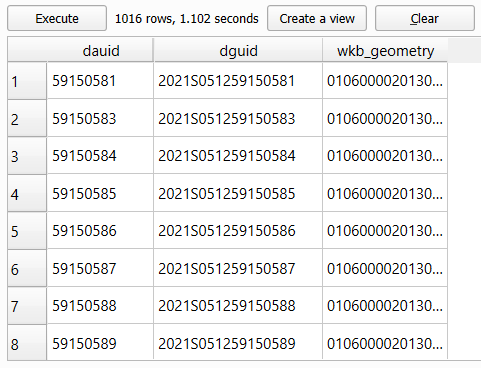
\includegraphics[width=0.75\linewidth]{images/05-qgis-query}

If you want, you can toggle on ``Load as a new layer'', set ``Column(s) with unique values'' to ``dauid'', set ``Geometry column'' to ``wkb\_geometry'', and click the ``Load'' button to temporarily load the query into your map to inspect it. This is not going to be our final layer yet, as we still need to join the appropriate census data to the geographic features.

\textbf{Step 4:} Open the psql shell and connect to the \texttt{greenequity} database on the UBC PostgreSQL server using the credential that you have been provided. Use the following query to return the first 20 rows of the ``census2021'' table:

\begin{Shaded}
\begin{Highlighting}[]
\KeywordTok{SELECT} \OperatorTok{*} \KeywordTok{FROM}\NormalTok{ census2021 }\KeywordTok{LIMIT} \DecValTok{20}\NormalTok{;}
\end{Highlighting}
\end{Shaded}

Do you notice that the data are oddly formatted? Notably, the first eight columns have repeating information, including the primary key ``DGUID''! This data organization is known as \textbf{long-format} and is useful when storing highly-dimensional data, and the census data you are working with have 2,631 dimensions!

Think of long-format as a list. Each row represents a new entry that holds a value or several values for a given observation-dimension pair. The advantage here is that if we do not have a value for a particular dimension for a particular observation, then we do not need to record anything, the row does not exist. Another advantage is that most relational database management systems have a limit on the number of columns that can be stored in a single table. For PostgreSQL, that limit is 1,600 columns compared to 255 for Microsoft Access databases, 1,024 for Microsoft SQL Server databases, and 1,000 for Oracle databases, just to name a few. However, there is practically no upper limit to the number of rows that can be stored in any of these databases.

This is a bit odd, because for most data analysis we are accustomed to seeing \textbf{wide-format} data where each row represents a unique feature that is described by many dimensions across the columns.

\textbf{Step 5:} Use the following query to return a table of population in the first 10 DGUIDs:

\begin{Shaded}
\begin{Highlighting}[]
\KeywordTok{SELECT}\NormalTok{ alt\_geo\_code, }\FunctionTok{MAX}\NormalTok{(c1\_count\_total) }\KeywordTok{FILTER}\NormalTok{ (}\KeywordTok{WHERE}\NormalTok{ characteristic\_id }\OperatorTok{=} \DecValTok{1}\NormalTok{) }\KeywordTok{AS}\NormalTok{ population }
\KeywordTok{FROM}\NormalTok{ census2021 }
\KeywordTok{GROUP} \KeywordTok{BY}\NormalTok{ alt\_geo\_code }
\KeywordTok{LIMIT} \DecValTok{10}\NormalTok{;}
\end{Highlighting}
\end{Shaded}

In this query, we are aggregating and grouping the data values back into our customary wide-format. We use the \texttt{MAX} aggregation function, though any other aggregation function would work since for any given dimension-observation there is only one value, so nearly any aggregation function applied to a single value would return that value (e.g., \texttt{max}, \texttt{min}, \texttt{avg}, \texttt{sum}). The reason for using the aggregation function at all is because the \texttt{FILTER} keyword will only apply aggregation functions to the predicate that follows \texttt{(WHERE\ characteristic\_id\ =\ 1)}. Finally, \texttt{GROUP\ BY\ alt\_geo\_code} ensures that the output table lists the populations for each \texttt{alt\_geo\_code}.

\hypertarget{a-word-about-alt_geo_code}{%
\subsection{A word about alt\_geo\_code}\label{a-word-about-alt_geo_code}}

The \texttt{alt\_geo\_code} is an identifier for every unique geographic division for census data in Canada. Some codes are shorter or longer than others, and this signifies the level in the geographic division hierarchy. For example, \texttt{alt\_geo\_code\ =\ 1} is the code for the entire country of Canada. So the first row you see in the output table from the query you ran above is the total population \texttt{characteristic\_id\ =\ 1} of Canada in 2021. Since the \texttt{alt\_geo\_code} is numeric, it is more flexible to query with than the DGUID, which is alphanumerical. \texttt{alt\_geo\_code\ =\ 59} is the code for the province of British Columbia. Remember that the data we are working with is only a subset of the national census representing the province of British Columbia, so there are no other provincial codes represented here. The code structure is pretty easy to follow from here. Every other geographic subdivision in British Columbia will begin with 59 and depending on the level of the hierarchy, will contain a different number of digits:

\begin{itemize}
\item
  \texttt{alt\_geo\_code\ =\ 59} represents British Columbia in the \textbf{Provinces and Territories Unique Identifier (PRUID)}
\item
  \texttt{alt\_geo\_code\ =\ 5901} represents the first \texttt{01} \textbf{Census Division (CD)}
\item
  \texttt{alt\_geo\_code\ =\ 5901003} represents the third \texttt{003} \textbf{Census Subdivision (CSD)} in the first CD
\item
  \texttt{alt\_geo\_code\ =\ 59010100} represents the 100th \texttt{0100} \textbf{Dissemination Area (DA)} in the third CSD, in the first CD
\end{itemize}

Codes with 8 digits are therefore \textbf{Dissemination Area Unique Identifiers (DAUID)}, which you should recognize are the values we need to use to join the census data to the actual dissemination area polygons that we just extracted in QGIS.

\textbf{Step 6:} We can modify our earlier query slightly to ensure we are only dealing with DAs:

\begin{Shaded}
\begin{Highlighting}[]
\KeywordTok{SELECT}\NormalTok{ alt\_geo\_code, }\FunctionTok{MAX}\NormalTok{(c1\_count\_total) }\KeywordTok{FILTER}\NormalTok{ (}\KeywordTok{WHERE}\NormalTok{ characteristic\_id }\OperatorTok{=} \DecValTok{1}\NormalTok{) }\KeywordTok{AS}\NormalTok{ population }
\KeywordTok{FROM}\NormalTok{ census2021 }
\KeywordTok{WHERE}\NormalTok{ geo\_level }\OperatorTok{=} \StringTok{\textquotesingle{}Dissemination area\textquotesingle{}} 
\KeywordTok{GROUP} \KeywordTok{BY}\NormalTok{ alt\_geo\_code }
\KeywordTok{LIMIT} \DecValTok{10}\NormalTok{;}
\end{Highlighting}
\end{Shaded}

\textbf{Step 7:} Now modify the query above so that it will produce an output table that contains all of the characteristics listed in the table below. Some IDs are given in the table below. For the remainder, you are expected to find the correct ID. You may need to refer to the \href{./data/98-401-X2021006_English_meta.txt}{readme file} that is distributed with the 98-401-X2021006 table in order to identify the correct characteristic\_id, which is listed under ``Definitions / Footnotes'', ``Characteristic (2631)'', and ``Member''. The number appearing to the far left of the readme file corresponds to the \texttt{characteristic\_id} in the database.

\begin{longtable}[]{@{}
  >{\raggedright\arraybackslash}p{(\columnwidth - 6\tabcolsep) * \real{0.2466}}
  >{\raggedright\arraybackslash}p{(\columnwidth - 6\tabcolsep) * \real{0.2603}}
  >{\raggedright\arraybackslash}p{(\columnwidth - 6\tabcolsep) * \real{0.2466}}
  >{\raggedright\arraybackslash}p{(\columnwidth - 6\tabcolsep) * \real{0.2466}}@{}}
\toprule\noalign{}
\begin{minipage}[b]{\linewidth}\raggedright
Characteristic\_ID
\end{minipage} & \begin{minipage}[b]{\linewidth}\raggedright
Characteristic
\end{minipage} & \begin{minipage}[b]{\linewidth}\raggedright
Units
\end{minipage} & \begin{minipage}[b]{\linewidth}\raggedright
Name
\end{minipage} \\
\midrule\noalign{}
\endhead
\bottomrule\noalign{}
\endlastfoot
& Population, 2021 & Persons & population \\
& Population density per square kilometre & Persons per square kilometre & popdensity \\
& Total - Private households by household size - 100\% data & Families & households \\
& Average household size & Persons & hhsize \\
345 & Prevalence of low income based on the Low-income measure, after tax (LIM-AT) (\%) & \% & lowincome \\
2008 & Bachelor's degree or higher & Persons & education \\
& Average age of the population & Years & age \\
35 & 0 to 14 years & \% & children \\
37 & 65 years and over & \% & seniors \\
& Unemployment rate & \% & unemployment \\
113 & Median total income in 2020 among recipients (\$) & \$ & medianincome \\
392 & First official language spoken is neither English nor French & Persons & neitherenglishorfrench \\
398 & Mother tongue is a non-official language & Persons & nonofficiallanguage \\
1536 & Immigrants arriving in 2016-2021 & Persons & immigrants \\
\end{longtable}

Your output table should look like the image below:

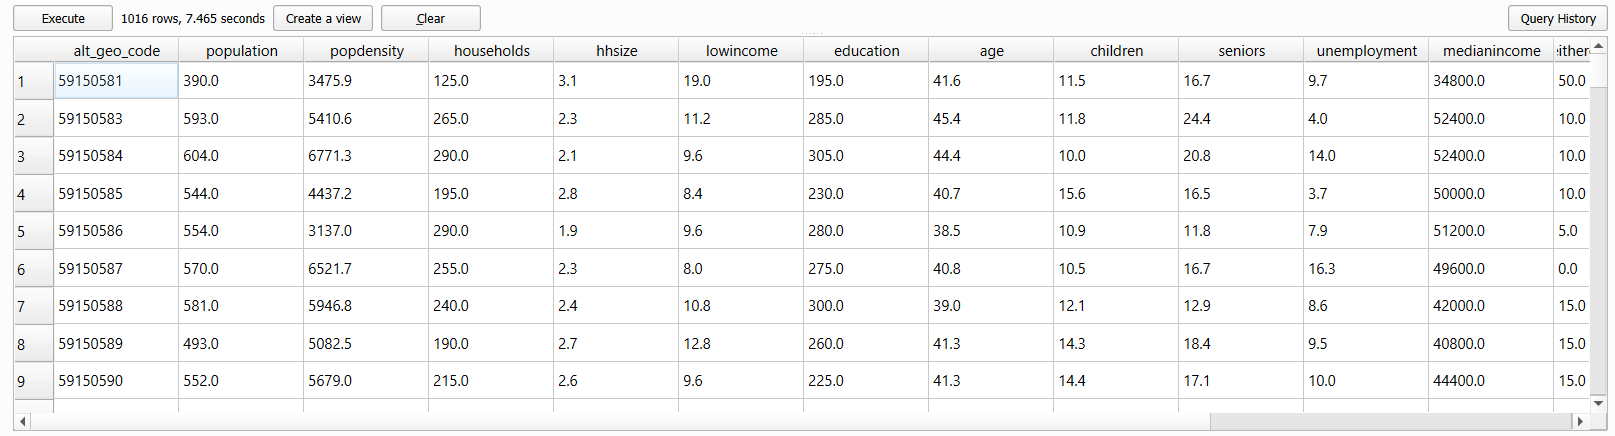
\includegraphics[width=0.75\linewidth]{images/05-qgis-query-characteristics}

\textbf{Step 8:} Finally, we are going to put everything together into a single SQL statement that will query, intersect, aggregate, group, and join the spatial data with the tabular data. Save your SQL query in QGIS Database Manager or copy it and paste it somewhere, then clear the SQL query area and paste the following statement:

\begin{Shaded}
\begin{Highlighting}[]
\KeywordTok{WITH} 

\CommentTok{{-}{-} Select the alt\_geo\_code and characteristics we want, aggregate and group them to convert to wide{-}format}

\NormalTok{characteristics }\KeywordTok{AS}\NormalTok{ (}
  \CommentTok{{-}{-} Insert your modified query from Step 7 here}
\NormalTok{),}

\CommentTok{{-}{-} Select the polygon geometry representing Vancouver from the Census Subdivisions (CSD)}

\NormalTok{vancouver }\KeywordTok{AS}\NormalTok{ (}
  \KeywordTok{SELECT}\NormalTok{ wkb\_geometry }
  \KeywordTok{FROM}\NormalTok{ lcsd000b21a\_e }
  \KeywordTok{WHERE}\NormalTok{ CSDNAME }\OperatorTok{=} \StringTok{\textquotesingle{}Vancouver\textquotesingle{}}
\NormalTok{),}

\CommentTok{{-}{-} Select the Dissemination Areas (DA) that are within the Vancouver CSD}

\NormalTok{vancouver\_da }\KeywordTok{AS}\NormalTok{ (}
  \KeywordTok{SELECT}\NormalTok{ lda\_000b21a\_e.DAUID, lda\_000b21a\_e.wkb\_geometry}
  \KeywordTok{FROM}\NormalTok{ vancouver, lda\_000b21a\_e}
  \KeywordTok{WHERE}\NormalTok{ ST\_Within(lda\_000b21a\_e.wkb\_geometry, vancouver.wkb\_geometry)}
\NormalTok{)}

\CommentTok{{-}{-} Perform the join of all the characteristics and the Vancouver DA geometries based on the DAUID}

\KeywordTok{SELECT}
\NormalTok{  characteristics.alt\_geo\_code,}
\NormalTok{  characteristics.population,}
\NormalTok{  characteristics.popdensity,}
\NormalTok{  characteristics.households,}
\NormalTok{  characteristics.hhsize,}
\NormalTok{  characteristics.lowincome,}
\NormalTok{  characteristics.education,}
\NormalTok{  characteristics.age,}
\NormalTok{  characteristics.children,}
\NormalTok{  characteristics.seniors,}
\NormalTok{  characteristics.unemployment,}
\NormalTok{  characteristics.medianincome,}
\NormalTok{  characteristics.neitherenglishorfrench,}
\NormalTok{  characteristics.nonofficiallanguage,}
\NormalTok{  characteristics.immigrants,}
\NormalTok{  vancouver\_da.wkb\_geometry}
\KeywordTok{FROM}
\NormalTok{  characteristics}
\KeywordTok{JOIN}
\NormalTok{  vancouver\_da }\KeywordTok{ON}\NormalTok{ characteristics.alt\_geo\_code:}\CharTok{:integer} \OperatorTok{=}\NormalTok{ vancouver\_da.DAUID:}\CharTok{:integer}\NormalTok{;}
\end{Highlighting}
\end{Shaded}

Be sure to add your modified statement from Step 7 where it is indicated. Then, the statement above should produce the final table we are looking for: a layer of dissemination areas for Vancouver that contain the values for the 14 characteristics we are interested in.

\includegraphics[width=0.75\linewidth]{images/05-qgis-final-query-load-layer}

\textbf{Step 9:} When you are satisfied, export the layer to your QGIS map and save it in your project folder (right-click the layer, ``Export'' \textgreater{} ``Save Features As\ldots{}''). We suggest exporting as shapefile format to maintain compatibility with ArcGIS Pro.

You may also want to save your SQL statement somewhere, too. You can use it later to recover all of your work from this task at any time from the PostgreSQL server. In QGIS, you can now play around with symbolizing the different characteristics. The image below shows population density \(\frac{persons}{km^2}\) of Vancouver dissemination areas in 2021 (projected coordinate system is Lambert Conformal Conic).

\includegraphics[width=0.75\linewidth]{images/05-qgis-population-density-vancouver-2021}

\textbf{Step 10:} Save you QGIS project.

\begin{center}\rule{0.5\linewidth}{0.5pt}\end{center}

\hypertarget{task-2-practice-geographically-weighted-regression}{%
\section*{Task 2: Practice geographically weighted regression}\label{task-2-practice-geographically-weighted-regression}}
\addcontentsline{toc}{section}{Task 2: Practice geographically weighted regression}

In this task, we are going to calculate the distance of each dissemination area to the nearest park in Vancouver and then select characteristics from the census data that explain the local variation in proximity to green space. So the census characteristics are going to be our independent (explanatory) variables \(k\) and the calculated distance to green space is going to be the dependent (response) variable \(y_i\) for our geographically weighted regression:

\[
y_i=𝛽_0(u_i,v_i)+\sum_{k}^{}𝛽_𝑘(u_i,v_i) 𝑥_{𝑖𝑘}+ε _𝑖
\]

\(𝛽_0(u_i,v_i)\) is the local model intercept at position \((u_i,v_i)\)

\(𝛽_k(u_i,v_i)\) is the local coefficient (slope) of the \(k\)-th independent variable (census characteristic) at position \((u_i,v_i)\)

\(𝑥_{𝑖𝑘}\) is the local \(i\)-th observation of the \(k\)-th independent variable (census characteristic)

\(ε _𝒊\) is the local error term (residual) for the \(i\)-th prediction

All of the instructions that follow are written for ArcGIS Pro because we will be performing the geographically weighted regression in ArcGIS Pro. We suggest setting up a new project and copying the ``vancouver\_da\_characteristics'' shapefile that you produced in the previous task into that project folder.

\textbf{Step 1:} Connect to the \texttt{greenequity} database on the UBC PostgreSQL server. Add two Landsat raster images: \textbf{LC08\_L1TP\_047026\_20200814\_20210330\_02\_T1\_B4} and \textbf{LC08\_L1TP\_047026\_20200814\_20210330\_02\_T1\_B5}. These images represent bands 4 (red) and 5 (near-infrared), respectively, and were acquired on August 14, 2020, which is approximately when the 2021 census data were collected.

\textbf{Step 2:} Open the ``Raster Calculator'' tool and calculate the Normalized Difference Vegetation Index (NDVI) and save the output in your project geodatabase simply as ``ndvi'':

\[
NDVI=\frac{Band5-Band4}{Band5+Band4}
\]

\includegraphics[width=1\linewidth]{images/05-arcgis-ndvi}

\textbf{Step 3:} Now we need to summarize the NDVI values over the dissemination areas. Open the ``Zonal Statistics as Table'' tool and use ``vancouver\_da\_characteristics'' as the ``Input raster or feature zone data'', select ``alt\_geo\_co'' as the ``Zone field'', use ``ndvi'' as the ``Input value raster'', and name the ``Output table'' as ``ndvi\_zonal\_statistics''. Ensure that ``Statistics type'' is set to ``All'', leave the other fields as default and run the tool.

\includegraphics[width=0.75\linewidth]{images/05-arcgis-zonal-statistics}

This will produce a table that should look like the image below. The table contains summary statistics of NDVI calculated for each dissemination area. Now we need to join this table to the polygon feature class.

\includegraphics[width=0.75\linewidth]{images/05-arcgis-zonal-statistics-table}

\textbf{Step 4:} Right-click on the ``vancouver\_da\_characteristics'' layer in your Contents Pane and select ``Joins and Relates'', then ``Add Join''. The ``Input Table'' is ``vancouver\_da\_characteristics'' and the ``Join Table'' is ``ndvi\_zonal\_statistics''. Select the correct keys to join the tables. This is a one-to-one join. Map the output, below is an example of average NDVI.

\includegraphics[width=1\linewidth]{images/05-arcgis-ndvi-mean}

It is important to initially analyze our census characteristics \(k\) to determine which independent variables and combination of these variables have the strongest relationship with our dependent variable, NDVI \(y\). To conduct the initial analysis, we will use a tool called ``Exploratory Regression'', which is part of the Spatial Statistics Toolbox.

\textbf{Step 5:} Open the ``Exploratory Regression'' tool. Select ``vancouver\_da\_characteristics'' as your ``Input Features'' and ``ndvi\_zonal\_statistics.MEAN'' as your dependent variable. Select all of the census characteristics as your ``Candidate Explanatory Variables'', expand ``Search Criteria'' and change the ``Maximum Number of Explanatory Variables'' to 14 then run the tool with other fields as default.

\includegraphics[width=0.75\linewidth]{images/05-arcgis-exploratory-regression}

\emph{NOTE:} \emph{Some fields were truncated when we saved the ``vancouver\_da\_characteristics'' shapefile. It should still be apparent which fields to select, but some of the original names will not perfectly match.}

\textbf{Step 6:} When the tool has finished running, click ``View Details'' at the bottom and then click ``Messages''. Under the heading ``Highest adjusted R-squared results'', you can explore the modeled relationship between one or more independent variables and the dependent variable. You should see the adjusted R-squared plateau at 0.41 when using a model with seven independent variables. We can use the statistics like Akaike's Information Criterion (AICc), Jarque-Bera p-value (JB), and Max Variance Inflation Factor (VIF) to choose between similar models with different sets of independent variables. Be sure to copy-paste this output message to a notepad so that you can reference it later in your report.

\includegraphics[width=0.75\linewidth]{images/05-arcgis-exploratory-regression-results}

\textbf{Step 7:} Once you have selected a model, write down the independent variables that are used in the model. Open the ``Ordinary Least Squares (OLS)'' tool. The ``Input Feature Class'' is ``vancouverda\_characteristics'', ``Unique ID Field'' is ``vancouver\_da\_characteristcs.alt\_geo\_co'', name the ``Output Feature Class'' as ``ols\_mean\_ndvi'', set the ``Dependent Variable'' to ``ndvi\_zonal\_statistics.MEAN'', and then select all of the independent variables that you wrote down from the last step. Run the tool, then click ``View Details'', select ``Messages'', and copy-paste the output to a notepad to reference it later in your report.

\includegraphics[width=0.75\linewidth]{images/05-arcgis-ols}

\textbf{Step 8:} Open the ``Geographically Weighted Regression (GWR)'' tool and parameterize it the same as you did in the last step for OLS, but change ``Neighborhood Type'' to ``Number of neighbors'', change ``Neighborhood Selection Method'' to ``Golden search'', and set ``Minimum Number of Neighbors'' to 50 and ``Maximum Number of Neighbors'' to 250. Name the ``Output Features'' as ``gwr\_mean\_ndvi''. Again, select all of the independent variables that you wrote down from earlier then run the tool. The output will automatically be added to your map along with several charts. Doubling-clicking on a chart will open it.

\includegraphics[width=0.75\linewidth]{images/05-arcgis-variable-chart}

\textbf{Step 9:} Save you ArcGIS Pro project.

\begin{center}\rule{0.5\linewidth}{0.5pt}\end{center}

\hypertarget{task-3-analyze-your-own-census-characteristics}{%
\section*{Task 3: Analyze your own census characteristics}\label{task-3-analyze-your-own-census-characteristics}}
\addcontentsline{toc}{section}{Task 3: Analyze your own census characteristics}

Your final task for this lab is to repeat Steps 8 and 9 of Task 1, but this time, select 10 of your own census characteristics and then perform your own analysis using what you have learned in Task 2. We strongly recommend referring to the readme file and other metadata that are linked in the Data section of the lab.

\textbf{Step 1:} Select 10 different census characteristics than the 14 we worked with and repeat Steps 8 and 9 of Task 1. You will be expected to rationalize why you selected these 10 characteristics in your report.

\textbf{Step 2:} Run all 10 characteristics through the ``Exploratory Regression'' tool. Repeat this process with three different NDVI statistics (e.g., mean, max, min, standard deviation, etc.). Record the output message and refer to any statistics here to justify your choice of a final set of independent variables for your regressions.

\textbf{Step 3:} Using your selected subset of independent variables, run the ``Ordinary Least Squares (OLS)'' tool for each of the three dependent variables, NDVI statistics that you chose in Step 2. Record the output message and refer to these statistics when you compare your OLS results to your GWR results.

\textbf{Step 4:} Using your selected subset of independent variables, run the ``Geographically Weighted Regression (GWR)'' tool for each of the three dependent variables, NDVI statistics that you chose in Step 2. Record the output message and refer to these statistics when you compare your GWR results to your OLS results.

\textbf{Step 5:} Explore your GWR results and make maps of the following for each of the three different NDVI statistics that you will reference in your report:
- Standardized residuals
- Local R\^{}\{2\}

\textbf{Step 6:} Explore your GWR results and make a map of one ``Coefficient'' and one ``Std.Error'' for one of your independent variables. Reference these maps when you are explaining your results in your report.

\textbf{Step 7:} Answer the following questions in your report and refer to all the maps, tables, and figures you made in the previous steps:

\begin{itemize}
\tightlist
\item
  Compare and contrast the different NDVI statistics. Which statistic had the best model? What evidence do you have for that conclusion? Why do you think that relationship was the strongest?
\item
  Interpret one of your independent variables in one of your three NDVI statistics using the Std.Error and Coefficient map. What spatial patterns do you see? What do you think could be influencing this relationship?
\item
  What other factors (spatial or aspatial) might be contributing or confounding your analysis? In other words, what other data sources might you add/calculate or what methods might you change to improve your results?
\item
  What can you conclude about green equity among dissemnination areas in Vancouver?
\end{itemize}

You will be expected to rationalize why you selected these 10 characteristics in your report.

\begin{center}\rule{0.5\linewidth}{0.5pt}\end{center}

\hypertarget{summary-4}{%
\section*{Summary}\label{summary-4}}
\addcontentsline{toc}{section}{Summary}

Geographically weighted regression can be a powerful tool for exploring spatial relationships. It takes some care and practice learning to interpret the many statistics along the journey, but it is one of the statistical methods that is rewarding to map and visualize. You should think of geographically weighted regression as a first approach at looking at a problem. It is great for exploring relationships, but not necessarily testing them. As you have seen, geographically weighted regression is a wonderful way to generate spatial hypotheses about data and explore the underlying tendencies of different relationships. Along the way, you have also learned how to wield high-dimensional census data in a database. Census data pair well with a wide variety of spatial analyses once you have decoded and unlocked their spatial mysteries.

Return to the \protect\hyperlink{lab5-deliverables}{\textbf{Deliverables}} section to check off everything you need to submit for credit in the course management system.

\end{document}
